% Compilation process:
% make compile
% or
% make book

\documentclass[fullbook]{tufte_algorithms_book}

% Remove empty pages (better for online PDF version)
\let\cleardoublepage\clearpage

% Chapter command without \newpage beforehand.
\newcommand{\inlinechapter}[1]{{\let\cleardoublepage\relax \chapter{#1}}}

% shared preamble code


% Removes empty pages
% \let\cleardoublepage\clearpage


%%% PSET and quiz settings:
\newcounter{pset}
\newcommand{\newpset}{\stepcounter{pset}}
\newcounter{quiz}
\newcommand{\newquiz}{\stepcounter{quiz}}



%%% Packages:
\usepackage{datetime}
\usepackage[titletoc,title]{appendix}
\usepackage{enumitem}
\usepackage{wrapfig}
\usepackage{nameref}
\usepackage{longtable,tabularx,booktabs}
\usepackage[flushleft]{threeparttable}
\usepackage{centernot}
\usepackage[outline]{contour} % for outlining text.
\usepackage{array}
\usepackage[makeroom]{cancel}
\usepackage{ifthen}
\usepackage[usestackEOL]{stackengine}
\usepackage{lipsum}
\usepackage{xcolor}
\usepackage{amsmath,amssymb,mathtools,bm,etoolbox}
\usepackage{multirow}
\usepackage{framed}
% \usepackage{minted}

%%% Package settings:
\newdateformat{psetdate}{\monthname[\the\month] \the\day,  \the\year}


%%% Custom commands
\definecolor{stanfordred}{RGB}{140,21,21}
\definecolor{darkgreen}{RGB}{21,140,21}
\definecolor{darkblue}{RGB}{21,21,140}
\definecolor{sun}{RGB}{234,171,0}
\colorlet{shadecolor}{black!5}

% \newcommand{\smallcaps}[1]{\textsc{#1}} % defined by tufte
\newcommand\euler{ℯ} % not working.
\makeatletter
\newcommand*{\currentname}{\@currentlabelname}
\makeatother

% \newcommand{\red}[1]{{\color{red} #1}} % ENABLED
\newcommand{\red}[1]{#1} % DISABLED

% \newcommand{\blue}[1]{{\color{blue} #1}} % ENABLED
\newcommand{\blue}[1]{#1} % DISABLED

\newcommand{\darkblue}[1]{{\color{darkblue} #1}} % ENABLED
% \newcommand{\darkblue}[1]{#1} % DISABLED

% \newcommand{\green}[1]{{\color{darkgreen} #1}} % ENABLED
\newcommand{\green}[1]{#1} % DISABLED

\newcommand{\darkgreen}[1]{{\color{darkgreen} #1}} % ENABLED
% \newcommand{\darkgreen}[1]{#1} % DISABLED

\newcommand{\darkred}[1]{{\color{stanfordred} #1}} % ENABLED
% \newcommand{\darkred}[1]{#1} % DISABLED

\newcommand{\br}{\phantom{ }}
% \newcommand{\snote}[1]{\sidenote[][0pt]{#1}}
\renewcommand{\cite}[2][0pt]{\sidenote[][#1]{\fullcite{#2}.}}

\newcommand{\ra}[1]{\renewcommand{\arraystretch}{#1}}
\newcommand\tab[1][1cm]{\hspace*{#1}}
\newcommand\tabhead[1]{\small\textbf{#1}}

\let\oparagraph\paragraph
\renewcommand{\paragraph}[1]{\oparagraph{\textbf{#1.}}}
\newcommand{\bparagraph}[1]{\oparagraph{\upshape \textbf{#1}}}

\newenvironment{problem}{%
	\begin{fullwidth}
}{%
	\end{fullwidth}
}

\newenvironment{answer}{%
	\begin{mdframed}[backgroundcolor=black!5,rightline=false,leftline=false]
		\vspace{-\baselineskip}
		\oparagraph{\textbf{Answer.}}
}{%
	\end{mdframed}
}

\newenvironment{overflowexample}{%
	\begin{mdframed}[backgroundcolor=black!5,rightline=false,leftline=false]
		\vspace{-\baselineskip}
}{%
	\end{mdframed}
}

% For Honor Code signing.
% \newcommand{\blank}{\hrulefill{}}
\newcommand{\ulfrule}{\xleaders\hbox{\underline{ }}\hfill\kern0pt}


% https://tex.stackexchange.com/questions/369890/combining-equation-number-with-tag-and-referencing-both-independently
\newcommand{\owntag}[1]{\stepcounter{equation}\tag{\theequation, #1}}

% Shorthand url without http(s)
\newcommand\rurl[1]{%
  \href{https://#1}{\nolinkurl{#1}}%
}


%% from preamble.tex of prob_reference.tex
\newenvironment{boxpar}
{
    \hspace*{0mm}
    \begin{tabular}{|p{0.95\textwidth}|}
    \hline
}
{
    \\[2mm]\hline
    \end{tabular}
    \vspace*{0mm}
} % boxes around paragraphs with titles


% Used for Julia algorithm blocks inside floats (i.e. examples)
\newenvironment*{exalgorithm}{}{}

% See pythontex.sty: https://github.com/sisl/tufte_algorithms_book/issues/16

% Expectation: https://tex.stackexchange.com/questions/229023/expectation-operator
\providecommand\given{}
\DeclarePairedDelimiterXPP\bbE[1]{\mathbb{E}}{[}{]}{}{
\renewcommand\given{  \nonscript\:
  \delimsize\vert
  \nonscript\:
  \mathopen{}
  \allowbreak}
#1
}


%%% Mathematical operators
%%% Mathematical operators
\DeclareMathOperator{\Var}{Var}
\DeclareMathOperator{\SD}{SD}
\DeclareMathOperator{\Ber}{Ber}
\DeclareMathOperator{\Bin}{Bin}
\DeclareMathOperator{\Poi}{Poi}
\DeclareMathOperator{\Geo}{Geo}
\DeclareMathOperator{\NegBin}{NegBin}
\DeclareMathOperator{\Uni}{Uni}
\DeclareMathOperator{\Exp}{Exp}
\DeclareMathOperator{\Dir}{Dir}
\newcommand*\Eval[1]{\left.#1\right\rvert} % derivative/integration evaluation bar |
\DeclareMathOperator{\Cov}{Cov}
\DeclareMathOperator{\BetaDistribution}{Beta}
\DeclareMathOperator{\Beta}{Beta}
\DeclareMathOperator{\GammaDist}{Gamma}
\DeclareMathOperator{\Gumbel}{Gumbel}
\DeclareMathOperator{\Std}{Std}
% \DeclareMathOperator{\Dirichlet}{Dir}
\DeclareMathOperator{\Train}{\mathcal{D}_{\text{train}}}
\DeclareMathOperator{\Dtrain}{\mathcal{D}_{\text{train}}}
% \newcommand{\Dtrain}{\mathcal{D}_\text{train}}
\DeclareMathOperator{\TrainLoss}{TrainLoss}
\DeclareMathOperator{\Loss}{Loss}
\DeclareMathOperator{\ZeroOneLoss}{Loss_{0\text{-}1}}
\DeclareMathOperator{\SquaredLoss}{Loss_{\text{squared}}}
\DeclareMathOperator{\AbsDevLoss}{Loss_{\text{absdev}}}
\DeclareMathOperator{\HingeLoss}{Loss_{\text{hinge}}}
\DeclareMathOperator{\LogisticLoss}{Loss_{\text{logistic}}}
\newcommand{\bfw}{\mathbf{w}}
\newcommand{\bbI}{\mathbb{I}}
\newcommand{\E}{\mathbb{E}}
\renewcommand{\cal}[1]{\mathcal{#1}}
\newcommand{\bb}[1]{\mathbb{#1}}
\DeclareMathOperator{\Miss}{Miss}
\DeclareMathOperator{\sgn}{sgn}
\newcommand{\1}{\mathbb{1}}
% \newcommand{\R}{\mathbb{R}}
\renewcommand{\v}{\mathbf{v}}
\newcommand{\V}{\mathbf{V}}
\newcommand{\w}{\mathbf{w}}
\newcommand{\h}{\mathbf{h}}
\newcommand{\opt}{*}
\DeclareMathOperator{\States}{States}
\DeclareMathOperator{\StartState}{s_{\text{state}}}
\DeclareMathOperator{\Actions}{Actions}
\DeclareMathOperator{\Reward}{Reward}
\DeclareMathOperator{\IsEnd}{IsEnd}
\DeclareMathOperator{\Cost}{Cost}
\DeclareMathOperator{\FutureCost}{FutureCost}
\DeclareMathOperator{\Succ}{Succ}


% TODO?: Box around important definitions (\newcommand\definition)?
% TODO?: \card{..} instead of |..|
% TODO?: \bbE{..} dynamic \left[ \right]


%%% TikZ settings
\tikzset{
    func/.style = {rectangle, rounded corners=1, draw},
    partial/.style = {rectangle, darkgreen, font=\bfseries},
    input/.style = {rectangle},
    nnnode/.style = {circle, draw=black, fill=white, minimum size=16pt,},
}


%%% Algorithm settings
% Remove "end _X_" text
\algtext*{EndLoop}
% \algtext*{EndFor}
\algtext*{EndIf}
\algtext*{EndFunction}


\setcounter{tocdepth}{2} % show subsection in TOC

\title{Machine Learning}
\author[Moss]{Robert J. Moss}
\date{2021}

\begin{document}

\begin{jlcode}
	include("../../jl/support_code.jl")
\end{jlcode}

\frontmatter
\makeatletter
%% MOSS: reduce blank pages for PDF-only version of book
% \begin{titlepage}
% {\Huge
% \noindent
% \@title}
% \end{titlepage}

% \cleardoublepage

\thispagestyle{empty}
\vfill
{\Huge
\noindent
\@title
}\\[0.5in]
{\Large
\noindent
% \@author
}
\vfill
{\large
\noindent
Stanford, California
% The MIT Press\\
% Cambridge, Massachusetts\\
% London, England
}\\[1in]
\makeatother


% \thispagestyle{empty}
\begin{fullwidth}
\vfill
\noindent\\[3in]
\copyright\ 2019\ Massachusetts Institute of
Technology\\[0.2in]
All rights reserved. No part of this book may be reproduced in any
form by any electronic or mechanical means (including photocopying,
recording or information storage and retrieval)
without permission in writing from the publisher.\\[0.2in]
This book was set in \TeX\ Gyre Pagella by the authors in \LaTeX.\\
Printed and bound in the United States of America.\\[0.2in]
Library of Congress Cataloging-in-Publication Data is available.\\[0.2in]
ISBN: \\[0.2in]
 10\hspace{1em}9\hspace{1em}8\hspace{1em}7\hspace{1em}6\hspace{1em}5\hspace{1em}4\hspace{1em}3\hspace{1em}2\hspace{1em}1
\end{fullwidth}

\clearpage

% \thispagestyle{empty}
~\\[3in]
\begin{fullwidth}
\begin{center}
\Large \itshape Place a dedication here.
\end{center}
\end{fullwidth}

\forceheader{Contents}
\tableofcontents\label{cha:toc}

\chapter*{Acknowledgments}
\addcontentsline{toc}{chapter}{Acknowledgments}

This work is taken from the lecture notes for the course \textit{Machine Learning} at Stanford University, CS 229 (\rurl{cs229.stanford.edu}). % TODO: remove extra spaces between " . "
The contributors to the content of this work are Andrew Ng and Christopher R\'e---this collection is simply a typesetting of existing lecture notes with minor modifications and additions of working Julia implementations. We would like to thank the original authors for their contribution.
% The authors wish to thank the many individuals who have provided valuable feedback on early drafts of our manuscript, including
% Adam Adamson,
% Barry Barryson,
% Cindy Cindyson, and
% Daryl Darylson.
% In addition, it has been a pleasure working with our editor from the MIT Press in preparing this manuscript for publication.
In addition, we wish to thank Mykel Kochenderfer and Tim Wheeler for their contribution to the Tufte-Algorithms \LaTeX{} template, based off of \textit{Algorithms for Optimization}.\cite{Kochenderfer2019}
% TODO: AA222/CS361 mention/link?

% The style of this book was inspired by Edward Tufte.
% Among other stylistic elements, we adopted his wide margins and use of small multiples.
% In fact, the typesetting of this book is heavily based on the Tufte-LaTeX package by Kevin Godby, Bil Kleb, and Bill Wood.

% We have also benefited from the various open source packages on which this textbook depends.
% The typesetting of the code is done with the help of pythontex, which is maintained by Geoffrey Poore.
% Plotting is handled by pgfplots, which is maintained by Christian Feuers\"{a}nger.
% The book's color scheme was adapted from the Monokai theme by Jon Skinner of Sublime Text (\url{sublimetext.com}).
% For plots, we use the viridis colormap defined by St\'efan van der Walt and Nathaniel Smith.


\vspace{5ex}
\noindent\textsc{Robert J. Moss}\\
Stanford, Calif.\\
\psetdate\today
\vfill
\noindent Ancillary material is available on the template's webpage:\\
\noindent\url{https://github.com/sisl/textbook_template}

% Based on handouts by Mehran Sahami, Chris Piech, and Lisa Yan.
% Stanford University, CS109, Spring 2020
% \chapter*{Preface}
\addcontentsline{toc}{chapter}{Preface}

This book template provides a starting point upon which authors may freely build to generate their own textbook entirely in \LaTeX.
We used this setup for Algorithms for Optimization, and have continued to refine it for a new textbook on decision making under uncertainty.
The template allows for the direct compilation of a print-ready PDF, including support for figures, examples, and exercises.

This template is intended for textbook authors.
Use of the template assumes prior expose to \LaTeX.
This template uses the \texttt{tufte-book} class to provide wide side margins.

Fundamental to our textbooks are the algorithms, which are all implemented in the Julia programming language.
We have found the language to be ideal for specifying algorithms in human readable form.
Algorithms can be typeset in algorithm blocks, tested, and used to generate figures.
We use pygments and pythontex, including a custom pygments lexer and style.

We hope that you find this useful.

\vspace{5ex}
\noindent\textsc{Mykel J. Kochenderfer}\\
\textsc{Tim A. Wheeler}\\
Stanford, Calif.\\
June 20, 2019
\vfill
\noindent Ancillary material is available on the template's webpage:\\
\noindent\url{https://github.com/sisl/textbook_template}
\mainmatter

\titlespacing*{\part}{0pt}{-20pt}{30pt} % to fix table and plot together on the first page (SEE RESTORE AT BOTTOM)
\titlespacing*{\chapter}{0pt}{-10pt}{30pt}

\part{Supervised Learning} % DIFF: top-level "part" is Supervised Learning (while "Linear Regression" is a chapter)
\label{part:supervised_learning}

\marginnote{From CS229 Fall 2020, Tengyu Ma, Andrew Ng, Moses Charikar, \& Christopher R\'e, Stanford University.}


Let's start by talking about a few examples of supervised learning problems.
Suppose we have a dataset giving the living areas and prices of 47 houses
from Portland, Oregon:

\begin{table}[!h]
  \centering
  \caption{
    \label{tab:houses} Housing prices in Portland, OR.
  }
  \begin{tabular}{cc}
    \toprule
    Living area (feet$^2$) & Price (1000\$s) \\
    \midrule
    2104 & 400 \\
    1600 & 330 \\
    2400 & 369 \\
    1416 & 232 \\
    3000 & 540 \\
    $\vdots$ & $\vdots$ \\
    \bottomrule
  \end{tabular}
\end{table}

\phantom{} % extra newline space

We can plot this data:
\begin{figure}
    \caption{
        \label{fig:houses} Housing prices in Portland, OR.
    }
    \begin{jlcode}
    p = let
        data = CSV.read("..\\data\\portland-houses.csv", DataFrame; header=["area", "bedrooms", "price"])
        X = data[:area]
        Y = data[:price] ./ 1000

        Axis(Plots.Scatter(X, Y, style="mark=x"), title="housing prices", xlabel="square feet", ylabel="price (in \\\$1000)", xmax=5000, ymax=800)
    end
    plot(p)
    \end{jlcode}
    \begin{center}
        \plot{fig/portland_houses}
    \end{center}
\end{figure}


Given data like this, how can we learn to predict the prices of other houses
in Portland, as a function of the size of their living areas?

To establish notation for future use, we'll use $x^{(i)}$ to denote the ``input''
variables (living area in this example), also called input \textbf{features}, and $y^{(i)}$
to denote the ``output'' or \textbf{target} variable that we are trying to predict
(price). A pair $(x^{(i)}, y^{(i)})$ is called a \textbf{training example}, and the dataset
that we'll be using to learn---a list of $n$ training examples $\{(x^{(i)}, y^{(i)} );\; i =
1,\ldots,n\}$---is called a \textbf{training set}. Note that the superscript ``$(i)$'' in the
notation is simply an index into the training set, and has nothing to do with
exponentiation. We will also use $\cal X$ denote the space of input values, and $\cal Y$
the space of output values. In this example, $\cal X = \cal Y = \bb R$.

To describe the supervised learning problem slightly more formally, our
goal is, given a training set, to learn a function $h: \cal X \mapsto \cal Y$ so that $h(x)$ is a
``good'' predictor for the corresponding value of $y$. For historical reasons, this
function $h$ is called a \textbf{hypothesis}. Seen pictorially, the process is therefore
like this:

\begin{figure}
\begin{center}
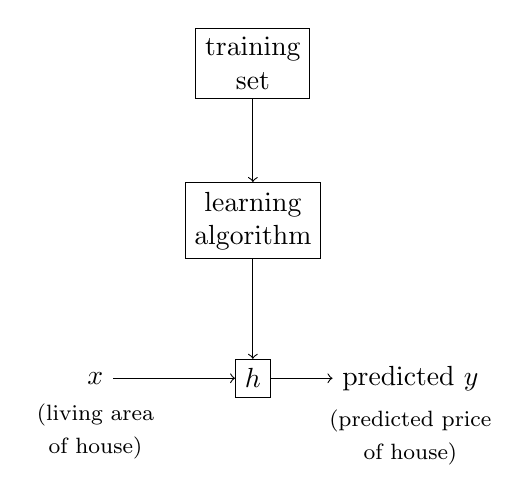
\begin{tikzpicture}[node distance=2cm, auto]
    \node [rectangle, align=center, draw] (training) {training\\set};
    \node [rectangle, align=center, draw, below of=training] (learning) {learning\\algorithm};
    \node [rectangle, align=center, draw, below of=learning] (h) {$h$};
    \node [left of=h, label={[align=center]below:\footnotesize (living area\\\footnotesize of house)}] (x) {$x$};
    \node [right of=h, label={[align=center]below:\footnotesize (predicted price\\\footnotesize of house)}] (y) {predicted $y$};

    \path [->, draw] (training) -- (learning);
    \path [->, draw] (learning) -- (h);
    \path [->, draw] (x) -- (h);
    \path [->, draw] (h) -- (y);
\end{tikzpicture}
\caption{\label{fig:hypothesis} Hypothesis diagram.}
\end{center}
\end{figure}

% TODO: get Francis Galton citation.
When the target variable that we're trying to predict is continuous, such
as in our housing example, we call the learning problem a \textbf{regression}\footnote{The term \textit{regression} was originally coined due to ``regressing'' to the mean (Francis Galton, 1886).} problem. % DIFF: regression term explanation.
When $y$ can take on only a small number of discrete values (such as
if, given the living area, we wanted to predict if a dwelling is a house or an
apartment, say), we call it a \textbf{classification} problem.


\chapter{Linear Regression}
\label{cha:linear_regression}

To make our housing example more interesting, let's consider a slightly richer
dataset in which we also know the number of bedrooms in each house:


\begin{table}[!h]
  \centering
  \caption{
    \label{tab:bedrooms} Housing prices with bedrooms in Portland, OR.
  }
  \begin{tabular}{ccc}
    \toprule
    Living area (feet$^2$) & \texttt{\#} Bedrooms & Price (1000\$s) \\
    \midrule
    2104 & 3 & 400 \\
    1600 & 3 & 330 \\
    2400 & 3 & 369 \\
    1416 & 2 & 232 \\
    3000 & 4 & 540 \\
    $\vdots$ & $\vdots$ & $\vdots$ \\
    \bottomrule
  \end{tabular}
\end{table}

Here, the $x$'s are two-dimensional vectors in $\bb R^2$. For instance, $x^{(i)}_1$
is the living area of the $i$-th house in the training set, and $x^{(i)}_2$
is its number of bedrooms.\footnote{In general, when designing a learning problem, it will be up to % DIFF: turned this parenthetical into a footnote
you to decide what features to choose, so if you are out in Portland gathering
housing data, you might also decide to include other features such as whether
each house has a fireplace, the number of bathrooms, and so on. We'll say
more about feature selection later, but for now let's take the features as
given.}

To perform supervised learning, we must decide how we're going to represent
functions/hypotheses $h$ in a computer. As an initial choice, let's say
we decide to approximate $y$ as a linear function of $x$:

\begin{equation}
    h_\theta(x) = \theta_0 + \theta_1 x_1 + \theta_2 x_2
\end{equation}

Here, the $\theta_i$'s are the \textbf{parameters} (also called \textbf{weights}) parameterizing the
space of linear functions mapping from $\cal X$ to $\cal Y$. When there is no risk of
confusion, we will drop the $\theta$ subscript in $h_\theta(x)$, and write it more simply as
$h(x)$. To simplify our notation, we also introduce the convention of letting
$x_0 = 1$ (this is the intercept term), so that
\begin{equation}
    h(x) = \sum_{i=0}^d \theta_i x_i = \theta^\top x\text{,} % DIFF: \top instead of ^T
\end{equation}
where on the right-hand side above we are viewing $\theta$ and $x$ both as vectors,
and here $d$ is the number of input variables (not counting $x_0$).

Now, given a training set, how do we pick, or learn, the parameters $\theta$?
One reasonable method seems to be to make $h(x)$ close to $y$, at least for
the training examples we have. To formalize this, we will define a function
that measures, for each value of the $\theta$'s, how close the $h(x^{(i)})$'s are to the
corresponding $y^{(i)}$'s. We define the \textbf{cost function}:

\begin{equation}
    J(\theta) = \frac 1 2 \sum_{i=1}^n \left( h_\theta(x^{(i)}) - y^{(i)} \right)^2\text{.}
\end{equation}

If you've seen linear regression before, you may recognize this as the familiar
least-squares cost function that gives rise to the \textbf{ordinary least squares}
regression model. Whether or not you have seen it previously, let's keep
going, and we'll eventually show this to be a special case of a much broader
family of algorithms.


\section{Least mean squares (LMS) algorithm} % DIFF: spelled out LMS

We want to choose $\theta$ so as to minimize $J(\theta)$. To do so, let's use a search
algorithm that starts with some ``initial guess'' for $\theta$, and that repeatedly
changes $\theta$ to make $J(\theta)$ smaller, until hopefully we converge to a value of
$\theta$ that minimizes $J(\theta)$. Specifically, let's consider the \textbf{gradient descent}
algorithm, which starts with some initial $\theta$, and repeatedly performs the
update:\footnote{This update is simultaneously performed for all values of $j = 0,\ldots,d$.} % DIFF: made parenthetical a footnote
%
\begin{equation}
    \theta_j \leftarrow \theta_j - \alpha \frac{\partial}{\partial \theta_j} J(\theta) % DIFF: Changed := to \leftarrow for update
\end{equation}
%
Here, $\alpha$ is called the \textbf{learning rate}. This is a very natural algorithm that
repeatedly takes a step in the direction of steepest decrease of $J$.

In order to implement this algorithm, we have to work out what is the
partial derivative term on the right hand side. Let's first work it out for the
case of if we have only one training example $(x,y)$, so that we can neglect
the sum in the definition of $J$. We have:

\begin{align*}
    \frac{\partial}{\partial \theta_j} J(\theta) &= \frac{\partial}{\partial \theta_j} \frac 1 2 \left( h_\theta(x) - y \right)^2\\
    &= 2 \cdot \frac 1 2 (h_\theta(x) - y) \cdot \frac{\partial}{\partial \theta_j} (h_\theta(x) - y) \\
    &= (h_\theta(x) - y) \cdot \frac{\partial}{\partial \theta_j} \left( \sum_{i=0}^d \theta_i x_i - y \right) \\
    &= (h_\theta(x) - y) x_j
\end{align*}

For a single training example, this gives the update rule:\footnote{We use the notation ``$a \leftarrow b$'' to denote an operation (in a computer program) in
which we set the value of a variable $a$ to be equal to the value of $b$ (something $:=$ is used). In other words, this
operation overwrites $a$ with the value of $b$. In contrast, we will write ``$a = b$'' when we are
asserting a statement of fact, that the value of $a$ is equal to the value of $b$.}

\begin{equation}
    \theta_j \leftarrow \theta_j + \alpha \left( y^{(i)} - h_\theta(x^{(i)}) \right) x^{(i)}_j \text{.} % DIFF: \leftarrow (:=)
\end{equation}

The rule is called the \textbf{LMS} update rule (LMS stands for ``least mean squares''),
and is also known as the \textbf{Widrow-Hoff} learning rule. This rule has several
properties that seem natural and intuitive. For instance, the magnitude of
the update is proportional to the \textbf{error} term $(y^{(i)} - h_\theta(x^{(i)}))$; thus, for
instance, if we are encountering a training example on which our prediction
nearly matches the actual value of $y^{(i)}$, then we find that there is little need
to change the parameters; in contrast, a larger change to the parameters will
be made if our prediction $h_\theta(x^{(i)})$ has a large error (i.e., if it is very far from
$y^{(i)}$).

We've derived the LMS rule for when there was only a single training % DIFF: we'd to we've
example. There are two ways to modify this method for a training set of
more than one example. The first is replace it with the following algorithm:

% DIFF: cleaned up this algorithm block (broke out the for loop).
\begin{algorithm}[ht]
    \caption{Gradient descent.}
    \label{alg:gd}
    \begin{algorithmic}
    \Repeat
        \For{every $j$}
            \State $\theta_j \leftarrow \theta_j + \alpha \displaystyle\sum\limits_{i=1}^n \left( y^{(i)} - h_\theta(x^{(i)}) \right) x^{(i)}_j$ %, \quad (for every $j$)
        \EndFor
    \Until{convergence}
    \end{algorithmic}
\end{algorithm}

By grouping the updates of the coordinates into an update of the vector
$\theta$, we can rewrite update \cref{alg:gd} in a slightly more succinct way:

\begin{algorithm}[ht]
    \caption{Gradient descent vectorized.}
    \label{alg:gd_vector}
    \begin{algorithmic}
    \Repeat
        \State $\theta \leftarrow \theta + \alpha \displaystyle\sum\limits_{i=1}^n \left( y^{(i)} - h_\theta(x^{(i)}) \right) x^{(i)}$
    \Until{convergence}
    \end{algorithmic}
\end{algorithm}

The reader can easily verify that the quantity in the summation in the
update rule above is just $\partial J(\theta) / \partial \theta_j$ (for the original definition of $J$).
So, this is simply gradient descent on the original cost function $J$. This method looks
at every example in the entire training set on every step, and is called \textbf{batch gradient descent}.
Note that, while gradient descent can be susceptible
to local minima in general, the optimization problem we have posed here
for linear regression has only one global, and no other local, optima; thus
gradient descent always converges (assuming the learning rate $\alpha$ is not too
large) to the global minimum. Indeed, $J$ is a convex quadratic function.


% TODO: Julia code (gradient descent—see alg4ai and "gradient_descent.jl")


\begin{example}
    \caption{\label{ex:gd} Gradient descent on a quadratic function.}

    Here is an example of gradient descent as it is run to minimize a quadratic
    function.

    \begin{jlcode}
    p = let
        @vars x, y
        f = x^2/2 + y^2
        plot_gradient_descent(f, initial=[48, 30], path_length=40)
    end
    plot(p)
    \end{jlcode}
    \begin{center}
        \plot{fig/gradient_descent}
    \end{center}

    The ellipses shown above are the contours of a quadratic function. Also
    shown is the trajectory taken by gradient descent, which was initialized at
    (48,30). The arrows in the figure (joined by straight lines) mark the successive % DIFF: changed $x$'s to arrows.
    values of $\theta$ that gradient descent went through.
\end{example}


\begin{example}
    % TODO: Generate \theta's directly from `linear_regression' (see plots-notebook.jl)
    When we run batch gradient descent to fit $\theta$ on our previous dataset,
    to learn to predict housing price as a function of living area. We obtain: % DIFF: split into two sentences.
    \begin{align*} % DIFF: put these in their own newlined equation block AND added \tag annotations.
        \theta_0 &= 71.27 \tag{intercept}\\
        \theta_1 &= 0.1345 \tag{slope}
    \end{align*}
    If we plot $h_\theta (x)$ as a function of $x$ (area), along
    with the training data, we obtain the following figure:

    \caption{
        % TODO I actually use linear regression here and not batch gradient descent.
        \label{ex:linear_regression} Best fit line using batch gradient descent on Portland, Oregon housing prices.
    }
    \begin{jlcode}
    p = let
        data = CSV.read("..\\data\\portland-houses.csv", DataFrame; header=["area", "bedrooms", "price"])
        X = data[:area]
        Y = data[:price] ./ 1000

        h = linear_regression(X, Y)

        p_data = Plots.Scatter(X, Y, style="mark=x")
        xn = (minimum(X) - 500):5000 # (maximum(X) + 500)

        p_fit = Plots.Linear(xn, h.(xn), style="blue, no marks")

        Axis([p_data, p_fit], title="housing prices", xlabel="square feet", ylabel="price (in \\\$1000)", xmin=first(xn), xmax=last(xn), ymax=800)
    end
    plot(p)
    \end{jlcode}
    \begin{center}
        \plot{fig/linear_regression}
    \end{center}

    % TODO: Generate \theta's directly from `linear_regression'
    If the number of bedrooms were included as one of the input features as well,
    we get $\theta_0 = 89.60, \theta_1 = 0.1392, \theta_2 = -8.738$.
\end{example}


% TODO: obtain these results with batch gradient descent.
The results in \cref{ex:linear_regression} were obtained with batch gradient descent. There is
an alternative to batch gradient descent that also works very well. Consider
the following algorithm:

% DIFF: Cleaned up the algorithm.
\begin{algorithm}[ht]
    \caption{Stochastic gradient descent.}
    \label{alg:sgd}
    \begin{algorithmic}
    \Repeat
        \For{$i = 1$ to $n$}
            \For{every $j$}
                \State $\theta_j \leftarrow \theta_j + \alpha \displaystyle\sum\limits_{i=1}^n \left( y^{(i)} - h_\theta(x^{(i)}) \right) x^{(i)}_j$ %, \quad (for every $j$)
            \EndFor
        \EndFor
    \Until{convergence}
    \end{algorithmic}
\end{algorithm}

By grouping the updates of the coordinates into an update of the vector
$\theta$, we can rewrite update in \cref{alg:sgd} in a slightly more succinct way:

\begin{equation}
    \theta \leftarrow \theta + \alpha \left( y^{(i)} - h_\theta^{(i)} \right) x^{(i)}
\end{equation}

In this algorithm, we repeatedly run through the training set, and each
time we encounter a training example, we update the parameters according
to the gradient of the error with respect to that single training example only.
This algorithm is called \textbf{stochastic gradient descent} (also \textbf{incremental
gradient descent}). Whereas batch gradient descent has to scan through
the entire training set before taking a single step---a costly operation if $n$ is
large---stochastic gradient descent can start making progress right away, and
continues to make progress with each example it looks at. Often, stochastic
gradient descent gets $\theta$ ``close'' to the minimum much faster than batch gradient
descent.\footnote{Note, however, that it may never ``converge'' to the minimum,
and the parameters $\theta$ will keep oscillating around the minimum of $J(\theta)$; but
in practice most of the values near the minimum will be reasonably good
approximations to the true minimum. By slowly letting the learning rate $\alpha$ decrease to
zero as the algorithm runs, it is also possible to ensure that the parameters will converge to
the global minimum rather than merely oscillate around the minimum.} % DIFF: combined parenthetical and footnote.
For these reasons, particularly when the training set is large,
stochastic gradient descent is often preferred over batch gradient descent.


\section{The normal equations}
\label{sec:the_normal_equations}

Gradient descent gives one way of minimizing $J$. Let's discuss a second way
of doing so, this time performing the minimization explicitly and without
resorting to an iterative algorithm. In this method, we will minimize $J$ by
explicitly taking its derivatives with respect to the $\theta_j$'s, and setting them to
zero. To enable us to do this without having to write reams of algebra and
pages full of matrices of derivatives, let's introduce some notation for doing
calculus with matrices.

\subsection{Matrix derivatives}
For a function $f : \bb R^{n \times d} \mapsto \bb R$ mapping from $n$-by-$d$ matrices to the real
numbers, we define the derivative of $f$ with respect to $A$ to be:

\begin{equation}
    \nabla_A f(A) = \begin{bmatrix}
        \frac{\partial f}{\partial A_{11}} & \cdots & \frac{\partial f}{\partial A_{1d}} \\
        \vdots & \ddots & \vdots \\
        \frac{\partial f}{\partial A_{n1}} & \cdots & \frac{\partial f}{\partial A_{nd}} \\
    \end{bmatrix}
\end{equation}

Thus, the gradient $\nabla_A f(A)$ is itself an $n$-by-$d$ matrix, whose $(i,j)$-element is
$\partial f / \partial A_{ij}$.

\begin{example}
    \caption{\label{ex:matrix_derivative}Matrix derivative.}

    For example, suppose $A =
    \begin{bmatrix}
        A_{11} & A_{12} \\
        A_{21} & A_{22}
    \end{bmatrix}$
    is a 2-by-2 matrix, and the function $f : \bb R^{2\times2} \mapsto \bb R$ is given by
    \begin{equation*}
        f(A) = \frac 3 2 A_{11} + 5 A_{12}^2 + A_{21}A_{22}\text{.}
    \end{equation*}
    Here, $A_{ij}$ denotes the $(i,j)$ entry of the matrix $A$. We then have:
    \begin{equation*}
        \nabla_A f(A) =
        \begin{bmatrix}
            \frac 3 2 & 10 A_{12} \\
            A_{22} & A_{21}
        \end{bmatrix}
    \end{equation*}
\end{example}


\subsection{Least squares revisited}

% TODO: \vec \theta ???? (CHANGE THROUGHOUT)

Armed with the tools of matrix derivatives, let us now proceed to find in
closed-form the value of $\theta$ that minimizes $J(\theta)$. We begin by re-writing $J$ in
matrix-vector notation. % DIFF: changed from "matrix-vectorial" to "matrix-vector"

% DIFF: bold-faced matrix $\mat X$
Given a training set, define the \textbf{design matrix} $\mat X$ to be the $n$-by-$d$ matrix
(actually $n$-by-$(d + 1)$, if we include the intercept term) that contains the % DIFF: added (...) around d+1
training examples' input values in its rows:

% DIFF: \top not ^T, bold-faced matrix (from here on out.)
\begin{equation}
    \mat X = \begin{bmatrix}
        \text{--- } (x^{(1)})^\top \text{ ---} \\
        \text{--- } (x^{(2)})^\top \text{ ---} \\
        \vdots \\
        \text{--- } (x^{(n)})^\top \text{ ---}
    \end{bmatrix}
\end{equation}
% DIFF: bold-face vector notation (not above-arrow, from here on out.)
Also, let $\vec y$ be the $n$-dimensional vector containing all the target values from
the training set:
\begin{equation}
    \vec y = \begin{bmatrix}
        y^{(1)} \\
        y^{(2)} \\
        \vdots \\
        y^{(n)}
    \end{bmatrix}
\end{equation}
Now, since $h_\theta(x^{(i)}) = (x^{(i)})^\top \theta$, we can easily verify that
\begin{align*}
    \mat X \theta - \vec y &= \begin{bmatrix}
        (x^{(1)})^\top \theta \\
        \vdots \\
        (x^{(n)})^\top \theta
    \end{bmatrix}
    -
    \begin{bmatrix}
        y^{(1)} \\    
        \vdots \\
        y^{(n)}    
    \end{bmatrix}\\
    &= \begin{bmatrix}
        h_\theta(x^{(1)}) - y^{(1)} \\
        \vdots \\
        h_\theta(x^{(n)}) - y^{(n)}
    \end{bmatrix}\text{.}
\end{align*}
Thus, using the fact that for a vector $z$, we have that $z^\top z = \sum_i z_i^2$:
\begin{align*}
    \frac 1 2 (\mat X \theta - \vec y)^\top (\mat X \theta - \vec y) &= \frac 1 2 \sum_{i=1}^n \left( h_\theta(x^{(i)}) - y^{(i)} \right)^2 \\
    &= J(\theta)
\end{align*}
Finally, to minimize $J$, let's find its derivative with respect to $\theta$. Hence:
\begin{align*}
    \nabla_\theta J(\theta) &= \nabla_\theta \frac 1 2 (\mat X \theta - \vec y)^\top (\mat X \theta - \vec y) \\
                            &= \frac 1 2 \nabla_\theta \left( (\mat X \theta)^\top \mat X \theta - (\mat X \theta)^\top \vec y - \vec y^\top (\mat X \theta) + \vec y^\top \vec y \right) \\
                            &= \frac 1 2 \nabla_\theta \left( \theta^\top (\mat X^\top \mat X) \theta - \vec y^\top (\mat X \theta) - \vec y^\top (\mat X \theta) \right) \tag{$a^\top b = b^\top a$} \\
                            &= \frac 1 2 \nabla_\theta \left( \theta^\top (\mat X^\top \mat X) \theta - 2 (\mat X^\top \vec y)^\top \theta \right) \\
                            &= \frac 1 2 \left( 2\mat X^\top \mat X \theta - 2 \mat X^\top \vec y \right) \tag{$\nabla_x b^\top x = b$ and $\nabla_x x^\top A x = 2 A x$ for sym. $A$} \\
                            &= \mat X^\top \mat X \theta - \mat X^\top \vec y
\end{align*}
% DIFF: Moved "third step" and "fifth step" explanations to \tags
To minimize $J$, we set its derivatives to zero, and obtain the \textbf{normal equations}:
\begin{equation}
    \mat X^\top \mat X \theta = \mat X^\top \vec y
\end{equation}
Thus, the value of $\theta$ that minimizes $J(\theta)$ is given in closed form by the equation:
\footnote{Note that in the this step, we are implicitly assuming that $\mat X^\top \mat X$ is an invertible
matrix. This can be checked before calculating the inverse. If either the number of
linearly independent examples is fewer than the number of features, or if the features
are not linearly independent, then $\mat X^\top \mat X$ will not be invertible. Even in such cases, it is
possible to ``fix'' the situation with additional techniques, which we skip here for the sake of simplicty.}
\begin{equation}
    \theta = (\mat X^\top \mat X)^{-1} \mat X^\top \vec y
\end{equation}


\section{Probabilistic interpretation}
When faced with a regression problem, why might linear regression, and
specifically why might the least-squares cost function $J$, be a reasonable
choice? In this section, we will give a set of probabilistic assumptions, under
which least-squares regression is derived as a very natural algorithm.

Let us assume that the target variables and the inputs are related via the
equation
\begin{equation}
    y^{(i)} = \theta^\top x^{(i)} + \epsilon^{(i)}\text{,}
\end{equation}
where $\epsilon^{(i)}$ is an error term that captures either unmodeled effects (such as
if there are some features very pertinent to predicting housing price, but
that we'd left out of the regression), or random noise. Let us further assume
that the $\epsilon^{(i)}$ are distributed IID (independently and identically distributed)
according to a Gaussian distribution (also called a Normal distribution) with
mean zero and some variance $\sigma^2$. We can write this assumption as % DIFF: removed quotes
$\epsilon^{(i)} \sim \cal N(0, \sigma^2)$, i.e. the density of $\epsilon^{(i)}$ is given by
\begin{equation}
    p(\epsilon^{(i)}) = \frac{1}{\sqrt{2\pi}\sigma} \exp \left( - \frac{(\epsilon^{(i)})^2}{2\sigma^2} \right)\text{.}
\end{equation}
This implies that
\begin{equation}
    p(y^{(i)} \mid x^{(i)}; \theta) = \frac{1}{\sqrt{2\pi}\sigma} \exp \left( - \frac{(y^{(i)} - \theta^\top x^{(i)})^2}{2\sigma^2} \right)\text{.}
\end{equation}
The notation ``$p(y^{(i)} \mid x^{(i)}; \theta)$'' indicates that this is the distribution of $y^{(i)}$
given $x^{(i)}$ and parameterized by $\theta$. Note that we should not condition on $\theta$
(i.e. ``$p(y^{(i)} \mid x^{(i)}, \theta)$''), since $\theta$ is not a random variable. We can also write the
distribution of $y^{(i)}$ as $(y^{(i)} \mid x^{(i)}; \theta) \sim \cal N(\theta^\top x^{(i)}, \sigma^2)$. % DIFF: added parens

Given $\mat X$ (the design matrix, which contains all the $x^{(i)}$'s) and $\theta$, what
is the distribution of the $y^{(i)}$'s? The probability of the data is given by
$p(\vec y \mid \mat X; \theta)$. This quantity is typically viewed a function of $\vec y$ (and perhaps $\mat X$),
for a fixed value of $\theta$. When we wish to explicitly view this as a function of
$\theta$, we will instead call it the \textbf{likelihood} function:
\begin{equation}
    L(\theta) = L(\theta; \mat X, \vec y) = p(\vec y \mid \mat X; \theta) %DIFF: removed period.
\end{equation}
Note that by the independence assumption on the $\epsilon^{(i)}$'s (and hence also the
$y^{(i)}$'s given the $x^{(i)}$'s), this can also be written as %DIFF: added "as"
\begin{align}
    L(\theta) &= \prod_{i=1}^n p(y^{(i)} \mid x^{(i)}; \theta)\\
              &= \prod_{i=1}^n \frac{1}{\sqrt{2\pi}\sigma} \exp \left( - \frac{(y^{(i)} - \theta^\top x^{(i)})^2}{2\sigma^2} \right)\text{.}
\end{align}
Now, given this probabilistic model relating the $y^{(i)}$'s and the $x^{(i)}$'s, what
is a reasonable way of choosing our best guess of the parameters $\theta$? The
principal of \textbf{maximum likelihood} says that we should choose $\theta$ so as to
make the data as high probability as possible---i.e. we should choose $\theta$ to
maximize $L(\theta)$.

Instead of maximizing $L(\theta)$, we can also maximize any strictly increasing
function of $L(\theta)$. In particular, the derivations will be a bit simpler if we
instead maximize the \textbf{log likelihood} $\ell(\theta)$:
\begin{align*}
    \ell(\theta) &= \log L(\theta) \\
    &= \log \prod_{i=1}^n \frac{1}{\sqrt{2\pi}\sigma} \exp \left( - \frac{(y^{(i)} - \theta^\top x^{(i)})^2}{2\sigma^2} \right) \\
    &= \sum_{i=1}^n \log \frac{1}{\sqrt{2\pi}\sigma} \exp \left( - \frac{(y^{(i)} - \theta^\top x^{(i)})^2}{2\sigma^2} \right) \\
    &= n \log \frac{1}{\sqrt{2\pi}\sigma} - \frac{1}{\sigma^2} \cdot \frac{1}{2} \sum_{i=1}^n \left(y^{(i)} - \theta^\top x^{(i)} \right)^2 %DIFF: no period.
\end{align*}
Hence, maximizing $\ell(\theta)$ gives the same answer as minimizing
\begin{equation*}
    \frac 1 2 \sum_{i=1}^n \left( y^{(i)} - \theta^\top x^{(i)} \right)^2\text{,}
\end{equation*}
which we recognize to be $J(\theta)$, our original least-squares cost function.

\paragraph{To summarize} Under the previous probabilistic assumptions on the data,
least-squares regression corresponds to finding the maximum likelihood estimate
of $\theta$. This is thus one set of assumptions under which least-squares regression
can be justified as a very natural method that's just doing maximum
likelihood estimation.\footnote{Note however that the probabilistic assumptions are
by no means necessary for least-squares to be a perfectly good and rational
procedure, and there may---and indeed there are---other natural assumptions
that can also be used to justify it.} % DIFF: footnote instead of parenthetical

Note also that, in our previous discussion, our final choice of $\theta$ did not
depend on what was $\sigma^2$, and indeed we'd have arrived at the same result
even if $\sigma^2$ were unknown. We will use this fact again later, when we talk
about the exponential family and generalized linear models.


\section{Locally weighted linear regression}
Consider the problem of predicting $y$ from $x \in \bb R$. The leftmost figure below
shows the result of fitting a $y = \theta_0 + \theta_1 x$ to a dataset. We see that the data
doesn't really lie on straight line, and so the fit is not very good.

\begin{figure*}
    \caption{
        \label{fig:polynomoial_regression} Polynomial regression with different $k$-order fits.
    }
    \begin{jlcode}
    p = let
        D = [(1,1), (2,2), (3,3), (4,3.25), (5,3.5), (6,3.75)]

        g = GroupPlot(3, 1, style="width=0.3\\textwidth")
        push!(g, plot_polynomial_regression(D, 1))
        push!(g, plot_polynomial_regression(D, 2))
        push!(g, plot_polynomial_regression(D, 5))
        g
    end
    plot(p)
    \end{jlcode}
    \begin{center}
        \plot{fig/polynomial_regression}
    \end{center}
\end{figure*}

Instead, if we had added an extra feature $x^2$, and fit $y = \theta_0 + \theta_1 x + \theta_2 x^2$,
then we obtain a slightly better fit to the data. (See middle figure) Naively, it
might seem that the more features we add, the better. However, there is also
a danger in adding too many features: The rightmost figure is the result of
fitting a 5-th order polynomial $y = \sum_{j=0}^5 \theta_j x^j$. We see that even though the
fitted curve passes through the data perfectly, we would not expect this to
be a very good predictor of, say, housing prices ($y$) for different living areas
($x$). Without formally defining what these terms mean, we'll say the figure
on the left shows an instance of \textbf{underfitting}---in which the data clearly
shows structure not captured by the model---and the figure on the right is
an example of \textbf{overfitting}.\footnote{Later in this class, when we talk about learning
theory we'll formalize some of these notions, and also define more carefully
just what it means for a hypothesis to be good or bad.} % DIFF: footnote from parenthetical

As discussed previously, and as shown in \cref{fig:polynomoial_regression}, the choice of %DIFF: \cref
features is important to ensuring good performance of a learning algorithm.
(When we talk about model selection, we'll also see algorithms for automatically
choosing a good set of features.) In this section, let us briefly talk
about the \textbf{locally weighted linear regression} (LWR) algorithm which, assuming
there is sufficient training data, makes the choice of features less critical.
This treatment will be brief, since you'll get a chance to explore some of the
properties of the LWR algorithm yourself in the homework.

In the original linear regression algorithm, to make a prediction at a query
point $x$ (i.e. to evaluate $h(x)$), we would: % DIFF: removed comma in i.e.
\begin{enumerate}
    \item Fit $\theta$ to minimize $\sum_i \left( y^{(i)} - \theta^\top x^{(i)} \right)^2$.
    \item Output $\theta^\top x$.
\end{enumerate}

In contrast, the locally weighted linear regression algorithm does the following:
\begin{enumerate}
    \item Fit $\theta$ to minimize $\sum_i w^{(i)} \left(y^{(i)} - \theta^\top x^{(i)} \right)^2$.
    \item Output $\theta^\top x$.
\end{enumerate}

Here, the $w^{(i)}$'s are non-negative valued \textbf{weights}. Intuitively, if $w^{(i)}$ is large
for a particular value of $i$, then in picking $\theta$ we'll try hard to make $(y^{(i)} - \theta^\top x^{(i)})^2$ small.
If $w^{(i)}$ is small, then the $(y^{(i)} - \theta^\top x^{(i)})^2$ error term will be
pretty much ignored in the fit.

A fairly standard choice for the weights is:% DIFF: footnote has equation blocks (moved w^{(i)} into sentence, outside of equations)
\footnote{If $x$ is vector-valued, the weights $w^{(i)}$ can be generalized to
\[\exp \left( - \frac{(x^{(i)} - x)^\top (x^{(i)} - x)}{2\tau^2} \right)\]
or
\[\exp \left( - \frac{(x^{(i)} - x)^\top \Sigma^{-1} (x^{(i)} - x)}{2\tau^2} \right)\]
for appropriate choices of $\tau$ or $\Sigma$.}
\begin{equation}
    w^{(i)} = \exp \left( - \frac{(x^{(i)} - x)^2}{2\tau^2} \right)
\end{equation}
Note that the weights depend on the particular point $x$ at which we're trying
to evaluate $x$. Moreover, if $\lvert x^{(i)} - x \rvert$ is small, then $w^{(i)}$ is close to 1; and
if $\lvert x^{(i)} - x \rvert$ is large, then $w^{(i)}$ is small. Hence, $\theta$ is chosen giving a much
higher ``weight'' to the (errors on) training examples close to the query point
$x$.\footnote{Note also that while the formula for the weights takes a form that is
cosmetically similar to the density of a Gaussian distribution, the $w^{(i)}$'s do
not directly have anything to do with Gaussians, and in particular the $w^{(i)}$
are not random variables, normally distributed or otherwise.} % DIFF: footnote instead of parenthetical
The parameter $\tau$ controls how quickly the weight of a training example falls off with distance
of its $x^{(i)}$ from the query point $x$; $\tau$ is called the \textbf{bandwidth} parameter, and
is also something that you'll get to experiment with in your homework.

Locally weighted linear regression is the first example we're seeing of a
\textbf{non-parametric} algorithm. The (unweighted) linear regression algorithm
that we saw earlier is known as a \textbf{parametric} learning algorithm, because
it has a fixed, finite number of parameters (the $\theta_i$'s), which are fit to the
data. Once we've fit the $\theta_i$'s and stored them away, we no longer need to
keep the training data around to make future predictions. In contrast, to
make predictions using locally weighted linear regression, we need to keep
the entire training set around. The term ``non-parametric'' (roughly) refers
to the fact that the amount of stuff we need to keep in order to represent the
hypothesis $h$ grows linearly with the size of the training set.



\chapter{Classification and Logistic Regression}
\label{cha:classification_logistic_regression}

Let's now talk about the classification problem. This is just like the regression
problem, except that the values $y$ we now want to predict take on only
a small number of discrete values. For now, we will focus on the \textbf{binary
classification} problem in which $y$ can take on only two values, $0$ and $1$.
(Most of what we say here will also generalize to the multiple-class case.)
For instance, if we are trying to build a spam classifier for email, then $x^{(i)}$
may be some features of a piece of email, and $y$ may be $1$ if it is a piece
of spam mail, and $0$ otherwise. The class $0$ is also called the \textbf{negative class}, and $1$ % DIFF: added "The class" to the sentence (don't start with numbers...)
the \textbf{positive class}, and they are sometimes also denoted by the symbols ``$-$''
and ``$+$''. Given $x^{(i)}$, the corresponding $y^{(i)}$ is also called the \textbf{label} for the
training example.

\section{Logistic regression} % NOTE Section 5.

\titlespacing*{\part}{0pt}{50pt}{40pt} % RESTORE
\titlespacing*{\chapter}{0pt}{50pt}{40pt} % RESTORE

We could approach the classification problem ignoring the fact that $y$ is
discrete-valued, and use our old linear regression algorithm to try to predict
$y$ given $x$. However, it is easy to construct examples where this method
performs very poorly. Intuitively, it also doesn't make sense for $h_\theta (x)$ to take
values larger than 1 or smaller than 0 when we know that $y \in \{0,1\}$.

To fix this, let's change the form for our hypotheses $h_\theta (x)$. We will choose
\[
h_\theta (x) = g(\theta^\top x) = \frac{1}{1 + e^{-\theta^\top x}}
\]
where
\[
g(z) = \frac{1}{1 + e^{-z}}
\]
is called the \textbf{logistic function} or the \textbf{sigmoid function}. Here is a plot
showing $g(z)$:

\begin{figure}
    \caption{
        \label{fig:sigmoid} Sigmoid function (i.e. logistic).
    }
    \begin{jlcode}
    p = let
        σ(z) = 1/(1 + exp(-z))
        X = -5:0.1:5
        Plots.Linear(X, σ.(X), style="blue, no marks")
    end
    plot(p)
    \end{jlcode}
    \begin{center}
        \plot{fig/sigmoid}
    \end{center}
\end{figure}

Notice that $g(z)$ tends towards $1$ as $z \to \infty$, and $g(z)$ tends towards $0$ as
$z \to -\infty$. Moreover, $g(z)$, and hence also $h(x)$, is always bounded between
$0$ and $1$. As before, we are keeping the convention of letting $x_0 = 1$, so that $\theta^\top x = \theta_0 + \sum_{j=1}^{d} \theta_j x_j$.

For now, let's take the choice of $g$ as given. Other functions that smoothly
increase from 0 to 1 can also be used, but for a couple of reasons that we'll see
later (when we talk about GLMs, and when we talk about generative learning
algorithms), the choice of the logistic function is a fairly natural one. Before
moving on, here's a useful property of the derivative of the sigmoid function,
which we write as $g'$:
\begin{align}
    g'(z) &= \frac{d}{dz}\frac{1}{1 + e^{-z}}\\
    &= \frac{1}{(1 + e^{-z})^2} (e^{-z})\\
    &= \frac{1}{(1 + e^{-z})} \cdot \left( 1 - \frac{1}{(1 + e^{-z})} \right)\\
    &= g(z)(1 - g(z))
\end{align}

So, given the logistic regression model, how do we fit $\theta$ for it? Following
how we saw least squares regression could be derived as the maximum likelihood
estimator under a set of assumptions, let's endow our classification
model with a set of probabilistic assumptions, and then fit the parameters
via maximum likelihood.

Let us assume that
\begin{align*}
    P(y = 1 \mid x;\theta) &= h_\theta (x)\\
    P(y = 0 \mid x;\theta) &= 1 - h_\theta (x)
\end{align*}
Note that this can be written more compactly as
\begin{equation}
    p(y \mid x;\theta) = (h_\theta (x))^y (1 - h_\theta (x))^{1-y}
\end{equation}
Assuming that the $n$ training examples were generated independently, we
can then write down the likelihood of the parameters as
\begin{align}
    L(\theta) &= p(\vec y \mid X;\theta)\\
    &= \prod^n_{i=1} p(y^{(i)} \mid x^{(i)} ;\theta)\\
    &= \prod^n_{i=1} \left( h_\theta(x^{(i)}) \right)^{y^{(i)}} \left( 1 - h_\theta (x^{(i)}) \right)^{1-y^{(i)}}
\end{align}
As before, it will be easier to maximize the log likelihood:
\begin{align}
    \ell(\theta) &= \log L(\theta)\\
    &= \sum_{i=1}^n y^{(i)} \log h(x^{(i)}) + (1 - y^{(i)})\log(1 - h(x^{(i)}))
\end{align}

How do we maximize the likelihood? Similar to our derivation in the case
of linear regression, we can use gradient ascent. Written in vectorial notation,
our updates will therefore be given by $\theta := \theta + \alpha \nabla_\theta \ell(\theta)$. (Note the positive
rather than negative sign in the update formula, since we're maximizing,
rather than minimizing, a function now.) Let's start by working with just
one training example $(x,y)$, and take derivatives to derive the stochastic
gradient ascent rule:
\begin{align}
    \frac{\partial}{\partial \theta_j}\ell(\theta) &=
    \left(y \frac{1}{g(\theta^\top x)} - (1-y) \frac{1}{1-g(\theta^\top x)} \right) \frac{\partial}{\partial \theta_j}g(\theta^\top x)\\
    &= \left(y \frac{1}{g(\theta^\top x)} - (1-y) \frac{1}{1-g(\theta^\top x)} \right) g(\theta^\top x) (1 - g(\theta^\top x)) \frac{\partial}{\partial \theta_j}\theta^\top x\\
    &= \left(y (1 - g(\theta^\top x)) - (1-y) g(\theta^\top x)\right) x_j\\
    &= (y - h_\theta(x)) x_j
\end{align}
Above, we used the fact that $g'(z) = g(z)(1 - g(z))$. This therefore gives us
the stochastic gradient ascent rule
\begin{equation}
    \theta_j := \theta_j + \alpha \left( y^{(i)} - h_\theta (x^{(i)}) \right) x^{(i)}_j
\end{equation}
If we compare this to the LMS update rule, we see that it looks identical; but
this is not the same algorithm, because $h_\theta (x^{(i)})$ is now defined as a non-linear
function of $\theta^\top x^{(i)}$. Nonetheless, it's a little surprising that we end up with
the same update rule for a rather different algorithm and learning problem.
Is this coincidence, or is there a deeper reason behind this? We'll answer this
when we get to GLM models.


\section{Digression: The perceptron learning algorithm} % TYPO: algorithn
We now digress to talk briefly about an algorithm that's of some historical
interest, and that we will also return to later when we talk about learning
theory. Consider modifying the logistic regression method to ``force'' it to
output values that are either 0 or 1 or exactly. To do so, it seems natural to
change the definition of g to be the threshold function:
\begin{equation}
    g(z) = \begin{cases}
        1 & \text{if } z \ge 0\\
        0 & \text{if } z < 0
    \end{cases}
\end{equation}
If we then let $h_\theta (x) = g(\theta^\top x)$ as before but using this modified definition of
$g$, and if we use the update rule
\begin{equation}
    \theta_j := \theta_j + \alpha \left( y^{(i)} - h_\theta (x^{(i)} ) \right) x^{(i)}_j    
\end{equation}
then we have the perceptron learning algorithm. % TYPO.

In the 1960s, this ``perceptron'' was argued to be a rough model for how
individual neurons in the brain work. Given how simple the algorithm is, it
will also provide a starting point for our analysis when we talk about learning
theory later in this class. Note however that even though the perceptron may
be cosmetically similar to the other algorithms we talked about, it is actually
a very different type of algorithm than logistic regression and least squares
linear regression; in particular, it is difficult to endow the perceptron's predic-
tions with meaningful probabilistic interpretations, or derive the perceptron
as a maximum likelihood estimation algorithm.


\section{Another algorithm for maximizing $\ell(\theta)$}

Returning to logistic regression with $g(z)$ being the sigmoid function, let's
now talk about a different algorithm for maximizing $\ell(\theta)$.

To get us started, let's consider Newton's method for finding a zero of a
function. Specifically, suppose we have some function $f : \mathbb R \mapsto \mathbb R$, and we
wish to find a value of $\theta$ so that $f(\theta) = 0$. Here, $\theta \in \mathbb R$ is a real number.
Newton's method performs the following update:
\begin{equation}
    \theta := \theta - \frac{f(\theta)}{f'(\theta)}
\end{equation}
This method has a natural interpretation in which we can think of it as
approximating the function $f$ via a linear function that is tangent to $f$ at
the current guess $\theta$, solving for where that linear function equals to zero, and
letting the next guess for $\theta$ be where that linear function is zero.

Here's a picture of the Newton's method in action:
\begin{figure*}
    \caption{
        \label{fig:newtons_method} Newton's method for two steps.
    }
    \begin{jlcode}
    p = plot_newtons_method()
    plot(p)
    \end{jlcode}
    \begin{center}
        \plot{fig/newtons_method}
    \end{center}
\end{figure*}

In the leftmost figure, we see the function f plotted along with the line
$y = 0$. We're trying to find $\theta$ so that $f(\theta) = 0$; the value of $\theta$ that achieves this
is about 1.3. Suppose we initialized the algorithm with $\theta = 4.5$. Newton's
method then fits a straight line tangent to $f$ at $\theta = 4.5$, and solves for the
where that line evaluates to 0. (Middle figure.) This give us the next guess
for $\theta$, which is about 2.8. The rightmost figure shows the result of running
one more iteration, which the updates $\theta$ to about 1.8. After a few more
iterations, we rapidly approach $\theta = 1.3$.

Newton's method gives a way of getting to $f(\theta) = 0$. What if we want to
use it to maximize some function $\ell$? The maxima of $\ell$ correspond to points
where its first derivative $\ell'(\theta)$ is zero. So, by letting $f(\theta) = \ell'(\theta)$, we can use
the same algorithm to maximize $\ell$, and we obtain update rule:
\begin{equation}
    \theta := \theta - \frac{\ell'(\theta)}{\ell^{\prime\prime}(\theta)}.
\end{equation}
(Something to think about: How would this change if we wanted to use
Newton's method to minimize rather than maximize a function?)

Lastly, in our logistic regression setting, $\theta$ is vector-valued, so we need to
generalize Newton's method to this setting. The generalization of Newton's
method to this multidimensional setting (also called the Newton-Raphson
method) is given by:
\begin{equation}
    \theta := \theta - H^{-1} \nabla_\theta \ell(\theta).
\end{equation}
Here, $\nabla_\theta \ell(\theta)$ is, as usual, the vector of partial derivatives of $\ell(\theta)$ with respect
to the $\theta_i$'s; and $H$ is an $d$-by-$d$ matrix (actually, $d+1$-by-$d+1$, assuming that
we include the intercept term) called the \textbf{Hessian}, whose entries are given by
\begin{equation}
    H ij = \frac{\partial^2 \ell(\theta)}{\partial\theta_i \partial\theta_j}.
\end{equation}

Newton's method typically enjoys faster convergence than (batch) gradient
descent, and requires many fewer iterations to get very close to the
minimum. One iteration of Newton's can, however, be more expensive than
one iteration of gradient descent, since it requires finding and inverting an
$d$-by-$d$ Hessian; but so long as $d$ is not too large, it is usually much faster
overall. When Newton's method is applied to maximize the logistic regression
log likelihood function $\ell(\theta)$, the resulting method is also called \textbf{Fisher
scoring}.



\chapter{Generalized Linear Models}

\marginnote{The presentation of the material in this section takes inspiration from Michael I.
Jordan, \textit{Learning in graphical models} (unpublished book draft), and also McCullagh and
Nelder, \textit{Generalized Linear Models} (2nd ed.).}

So far, we've seen a regression example, and a classification example. In the
regression example, we had $y \mid x; \theta \sim \mathcal{N}(\mu, \sigma^2)$, and in the classification one,
$y \mid x; \theta \sim \operatorname{Bernoulli}(\phi)$, for some appropriate definitions of $\mu$ and $\phi$ as functions
of $x$ and $\theta$. In this section, we will show that both of these methods are
special cases of a broader family of models, called \textit{Generalized Linear Models}
(GLMs). We will also show how other models in the GLM family can be
derived and applied to other classification and regression problems.

\section{The exponential family}
To work our way up to GLMs, we will begin by defining exponential family
distributions. We say that a class of distributions is in the exponential family
if it can be written in the form:
\[
p(y; \eta) = b(y)\exp(\eta^\top T(y) - a(\eta)) \label{eq:glm}
\]
Here, $\eta$ is called the \textbf{natural parameter} (also called the \textbf{canonical parameter})
of the distribution; $T(y)$ is the \textbf{sufficient statistic} (for the distributions
we consider, it will often be the case that $T(y) = y$); and $a(\eta)$ is the \textbf{log
partition function}. The quantity $e^{-a(\eta)}$ essentially plays the role of a normalization
constant, that makes sure the distribution $p(y;\eta)$ sums/integrates
over $y$ to 1.
\marginnote{MLE w.r.t. $\eta$ is concave $\rightarrow$ (neg. log-likelihood is convex)}

A fixed choice of $T$, $a$ and $b$ defines a family (or set) of distributions that
is parameterized by $\eta$; as we vary $\eta$, we then get different distributions within
this family.

We now show that the Bernoulli and the Gaussian distributions are examples
of exponential family distributions. The Bernoulli distribution with
mean $\phi$, written $\operatorname{Bernoulli}(\phi)$, specifies a distribution over $y \in \{0,1\}$, so that
$p(y = 1;\phi) = \phi; p(y = 0;\phi) = 1 - \phi$. As we vary $\phi$, we obtain Bernoulli
distributions with different means. We now show that this class of Bernoulli
distributions, ones obtained by varying $\phi$, is in the exponential family; i.e.,
that there is a choice of $T$, $a$ and $b$ so that \ref{eq:glm} becomes exactly the
class of Bernoulli distributions.

We write the Bernoulli distribution as:
\begin{align}
    p(y;\phi) &= \phi^y (1 - \phi)^{1-y}\\
              &= \exp(y \log\phi + (1 - y)\log(1 - \phi))\\
              &= \exp\left( y\left( \log\left(\frac{\phi}{1-\phi}\right)\right) + \log(1-\phi)\right).
\end{align}
Thus, the natural parameter is given by $\eta = \log(\phi/(1 - \phi))$. Interestingly, if
we invert this definition for $\eta$ by solving for $\phi$ in terms of $\eta$, we obtain $\phi =
1/(1 + e^{-\eta})$. This is the familiar sigmoid function! This will come up again
when we derive logistic regression as a GLM. To complete the formulation
of the Bernoulli distribution as an exponential family distribution, we also
have:
\begin{align*}
    T(y) &= y\\
    a(\eta) &= -\log(1 - \phi)\\
            &= \log(1 + e^{\eta})\\
    b(y) &= 1    
\end{align*}
This shows that the Bernoulli distribution can be written in the form of
\ref{eq:glm}, using an appropriate choice of $T$, $a$ and $b$.

Let's now move on to consider the Gaussian distribution. Recall that,
when deriving linear regression, the value of $\sigma^2$ had no effect on our final
choice of $\theta$ and $h_\theta (x)$. Thus, we can choose an arbitrary value for $\sigma^2$ without
changing anything. To simplify the derivation below, let's set $\sigma^2 = 1$.\footnote{If we leave $\sigma^2$ as a variable, the Gaussian distribution can also be shown to be in the exponential family, where $\eta \in \mathbb R^2$ is now a 2-dimension vector that depends on both $\mu$ and
$\sigma$. For the purposes of GLMs, however, the $\sigma^2$ parameter can also be treated by considering
a more general definition of the exponential family: $p(y;\eta,\tau) = b(a,\tau)\exp((\eta^\top T(y) - a(\eta))/c(\tau))$.
Here, $\tau$ is called the \textbf{dispersion parameter}, and for the Gaussian, $c(\tau) = \sigma^2$;
but given our simplification above, we won't need the more general definition for the
examples we will consider here.}
We then have:
\begin{align}
    p(y;\mu) &= \frac{1}{\sqrt{2\pi}}\exp\left(-\frac{1}{2} (y - \mu)^2\right)\\
             &= \frac{1}{\sqrt{2\pi}}\exp\left(-\frac{1}{2} y^2 \right) \cdot  \exp\left(\mu y - \frac{1}{2}\mu^2\right)
\end{align}
Thus, we see that the Gaussian is in the exponential family, with
\begin{align*}
    \eta &= \mu\\
    T(y) &= y\\
    a(\eta) &= \mu^2 / 2\\
            &= \eta^2 / 2\\
    b(y) &= (1 / \sqrt{2\pi})\exp(-y^2 / 2).
\end{align*}
There're many other distributions that are members of the exponential family:
The multinomial (which we'll see later), the Poisson (for modelling
count-data; also see the problem set); the gamma and the exponential
(for modelling continuous, non-negative random variables, such as time-intervals);
the beta and the Dirichlet (for distributions over probabilities);
and many more. In the next section, we will describe a general ``recipe''
for constructing models in which $y$ (given $x$ and $\theta$) comes from any of these
distributions.


\section{Constructing GLMs}
\marginnote{Inference is easy:
\[
\mathbb E[y; \eta] = \frac{\partial}{\partial \eta} a(\eta)
\]
(log partition of exp. family).
}
Suppose you would like to build a model to estimate the number $y$ of customers
arriving in your store (or number of page-views on your website) in
any given hour, based on certain features $x$ such as store promotions, recent
advertising, weather, day-of-week, etc. We know that the Poisson distribution
usually gives a good model for numbers of visitors. Knowing this, how
can we come up with a model for our problem? Fortunately, the Poisson is an
exponential family distribution, so we can apply a Generalized Linear Model
(GLM). In this section, we will we will describe a method for constructing
GLM models for problems such as these.

More generally, consider a classification or regression problem where we
would like to predict the value of some random variable $y$ as a function of
$x$. To derive a GLM for this problem, we will make the following three
assumptions about the conditional distribution of $y$ given $x$ and about our
model:
\begin{enumerate}
    \item $y \mid x;\theta \sim \operatorname{ExponentialFamily}(\eta)$. I.e., given $x$ and $\theta$, the distribution of
$y$ follows some exponential family distribution, with parameter $\eta$.
    \item Given $x$, our goal is to predict the expected value of $T(y)$ given $x$.
    In most of our examples, we will have $T(y) = y$, so this means we
    would like the prediction $h(x)$ output by our learned hypothesis $h$ to
    satisfy $h(x) = \mathbb E[y \mid x]$. (Note that this assumption is satisfied in the
    choices for $h_\theta (x)$ for both logistic regression and linear regression. For
    instance, in logistic regression, we had $h_\theta (x) = p(y = 1 \mid x;\theta) = 0 \cdot p(y =
        0 \mid x;\theta) + 1 \cdot p(y = 1 \mid x;\theta) = \mathbb E[y \mid x;\theta]$.)

    \item The natural parameter $\eta$ and the inputs $x$ are related linearly: $\eta = \theta^\top x$.
    (Or, if $\eta$ is vector-valued, then $\eta_i = \theta^\top_i x$.)
\end{enumerate}

The third of these assumptions might seem the least well justified of
the above, and it might be better thought of as a ``design choice'' in our
recipe for designing GLMs, rather than as an assumption per se. These
three assumptions/design choices will allow us to derive a very elegant class
of learning algorithms, namely GLMs, that have many desirable properties
such as ease of learning. Furthermore, the resulting models are often very
effective for modelling different types of distributions over $y$; for example, we
will shortly show that both logistic regression and ordinary least squares can
both be derived as GLMs.

\subsection{Ordinary Least Squares}
To show that ordinary least squares is a special case of the GLM family
of models, consider the setting where the target variable $y$ (also called the
\textbf{response variable} in GLM terminology) is continuous, and we model the
conditional distribution of $y$ given $x$ as a Gaussian $\mathcal N(\mu,\sigma^2)$. (Here, $\mu$ may
depend $x$.) So, we let the $\operatorname{ExponentialFamily}(\eta)$ distribution above be
the Gaussian distribution. As we saw previously, in the formulation of the
Gaussian as an exponential family distribution, we had $\mu = \eta$. So, we have
\begin{align*}
    h_\theta (x) &= \mathbb E[y \mid x;\theta]\\
    &= \mu\\
    &= \eta\\
    &= \theta^\top x.
\end{align*}
The first equality follows from Assumption 2, above; the second equality
follows from the fact that $y \mid x;\theta \sim \mathcal N(\mu,\sigma^2)$, and so its expected value is given
by $\mu$; the third equality follows from Assumption 1 (and our earlier derivation
showing that $\mu = \eta$ in the formulation of the Gaussian as an exponential
family distribution); and the last equality follows from Assumption 3.

\subsection{Logistic Regression}
We now consider logistic regression. Here we are interested in binary classification,
so $y \in \{0,1\}$. Given that $y$ is binary-valued, it therefore seems natural
to choose the Bernoulli family of distributions to model the conditional distribution
of $y$ given $x$. In our formulation of the Bernoulli distribution as
an exponential family distribution, we had $\phi = 1/(1 + e^{-\eta})$. Furthermore,
note that if $y \mid x;\theta \sim \operatorname{Bernoulli}(\phi)$, then $\mathbb E[y \mid x;\theta] = \phi$. So, following a similar
derivation as the one for ordinary least squares, we get:
\begin{align*}
    h_\theta (x) &= \mathbb E[y \mid x;\theta]\\
    &= \phi\\
    &= 1/(1 + e^{-\eta})\\
    &= 1/(1 + e^{-\theta^\top x})    
\end{align*}
So, this gives us hypothesis functions of the form $h_\theta (x) = 1/(1 + e^{-\theta^\top x})$. If
you are previously wondering how we came up with the form of the logistic
function $1/(1 + e^{-z})$, this gives one answer: Once we assume that $y$ conditioned
on $x$ is Bernoulli, it arises as a consequence of the definition of GLMs
and exponential family distributions.

To introduce a little more terminology, the function $g$ giving the distribution's
mean as a function of the natural parameter ($g(\eta) = \mathbb E[T(y); \eta]$)
is called the \textbf{canonical response function}. Its inverse, $g^{-1}$, is called the
\textbf{canonical link function}. Thus, the canonical response function for the
Gaussian family is just the identity function; % TYPO? identity not "identify"?
and the canonical response function for the Bernoulli is the logistic function.\footnote{Many texts use $g$ to denote the link function, and $g^{-1}$
to denote the response function; but the notation we're using here, inherited from the early machine learning literature,
will be more consistent with the notation used in the rest of the class.}

\subsection{Softmax Regression}
Let's look at one more example of a GLM. Consider a classification problem
in which the response variable $y$ can take on any one of $k$ values, so $y \in
\{1,2,\ldots,k\}$. For example, rather than classifying email into the two classes
spam or not-spam---which would have been a binary classification problem---
we might want to classify it into three classes, such as spam, personal mail,
and work-related mail. The response variable is still discrete, but can now
take on more than two values. We will thus model it as distributed according
to a multinomial distribution.

Let's derive a GLM for modelling this type of multinomial data. To do
so, we will begin by expressing the multinomial as an exponential family
distribution.

To parameterize a multinomial over $k$ possible outcomes, one could use
$k$ parameters $\phi_1 ,\ldots,\phi_k$ specifying the probability of each of the outcomes.
However, these parameters would be redundant, or more formally, they would
not be independent (since knowing any $k-1$ of the $\phi_i$'s uniquely determines
the last one, as they must satisfy $\sum_{i=1}^k \phi_i = 1$). So, we will instead parameterize
the multinomial with only $k - 1$ parameters, $\phi_1,\ldots,\phi_{k-1}$, where
$\phi_i = p(y = i;\phi)$, and $p(y = k;\phi) = 1 - \sum_{i=1}^{k-1} \phi_i$. For notational convenience,
we will also let $\phi_k = 1 - \sum_{i=1}^{k-1} \phi_i$, but we should keep in mind that this is
not a parameter, and that it is fully specified by $\phi_1,\ldots,\phi_{k-1}$.

To express the multinomial as an exponential family distribution, we will
define $T(y) \in \mathbb R^{k-1}$ as follows:
\begin{equation*}
    T(1) = \begin{bmatrix}1\\0\\0\\\vdots\\0\end{bmatrix},
    T(2) = \begin{bmatrix}0\\1\\0\\\vdots\\0\end{bmatrix},
    \cdots,
    T(k-1) = \begin{bmatrix}0\\0\\0\\\vdots\\1\end{bmatrix},
    T(k) = \begin{bmatrix}0\\0\\0\\\vdots\\0\end{bmatrix},
\end{equation*}
Unlike our previous examples, here we do \textit{not} have $T(y) = y$; also, $T(y)$ is
now a $k - 1$ dimensional vector, rather than a real number. We will write
$(T(y))_i$ to denote the $i$-th element of the vector $T(y)$.
We introduce one more very useful piece of notation. An indicator function
$\mathbb{1}\{\cdot\}$ takes on a value of 1 if its argument is true, and 0 otherwise
($\mathbb{1}\{\texttt{True}\} = 1$, $\mathbb{1}\{\texttt{False}\} = 0$). For example, $\mathbb{1}\{2 = 3\} = 0$, and $\mathbb{1}\{3 =
5 - 2\} = 1$. So, we can also write the relationship between $T(y)$ and $y$ as
$(T(y))_i = \mathbb{1}\{y = i\}$. (Before you continue reading, please make sure you understand
why this is true!) Further, we have that $\mathbb E[(T(y))_i] = P(y = i) = \phi_i$.

We are now ready to show that the multinomial is a member of the
exponential family. We have:
\begin{align*}
    p(y; \phi) &= \phi_1^{\mathbb{1}\{y=1\}} \phi_2^{\mathbb{1}\{y=2\}} \cdots \phi_k^{\mathbb{1}\{y=k\}}\\
               &= \phi_1^{\mathbb{1}\{y=1\}} \phi_2^{\mathbb{1}\{y=2\}} \cdots \phi_k^{1 - \sum_{i=1}^{k-1}\mathbb{1}\{y=i\}}\\
               &= \phi_1^{(T(y))_1} \phi_2^{(T(y))_2} \cdots \phi_k^{1 - \sum_{i=1}^{k-1}(T(y))_i}\\
               &= \exp\left((T(y))_i \log(\phi_1) + (T(y))_2 \log(\phi_2) + \cdots + \left(1 - \sum_{i=1}^{k-1} (T(y))_i \right) \log(\phi_k) \right)\\
               &= \exp\left((T(y))_i \log(\phi_1/\phi_k) + (T(y))_2 \log(\phi_2/\phi_k) + \cdots + (T(k))_{k-1} \log(\phi_{k-1}/\phi_k) + \log(\phi_k)\right)\\
               &= b(y) \exp(\eta^\top T(y) - a(\eta))
\end{align*}
where
\begin{align*}
    \eta &= \begin{bmatrix} \log(\phi_1 / \phi_k) \\ \log(\phi_2 / \phi_k) \\ \vdots \\ \log(\phi_{k-1}/\phi_k) \end{bmatrix},\\
    a(\eta) &= - \log(\phi_k)\\
    b(y) &= 1.
\end{align*}
This completes our formulation of the multinomial as an exponential family
distribution.

The link function is given (for $i = 1,\ldots,k$) by:
\[
\eta_i = \log \frac{\phi_i}{\phi_k}
\]
For convenience, we have also defined $\eta_k = \log(\phi_k / \phi_k) = 0$. To invert the
link function and derive the response function, we therefore have that
\begin{align}
    e^{\eta_i} &= \frac{\phi_i}{\phi_k}\\
    \phi_k e^{\eta_i} &= \phi_i\label{eq:resp_fnc}\\
    \phi_k \sum_{i=1}^k e^{\eta_i} &= \sum_{i=1}^k \phi_i = 1
\end{align}
This implies that $\phi_k = 1 / \sum_{i=1}^k e^{\eta_i}$, which can be substituted back into \cref{eq:resp_fnc} to give the response function
\[
\phi_i = \frac{e^{\eta_i}}{\sum_{j=1}^k e^{\eta_j}}
\]
This function mapping from the $\eta$'s to the $\phi$'s is called the \textbf{softmax} function.

To complete our model, we use Assumption 3, given earlier, that the $\eta_i$'s
are linearly related to the $x$'s. So, have $\eta_i = \theta^\top_i x$ (for $i = 1,\ldots, k-1$),
where $\theta_1,\ldots, \theta_{k-1} \in \mathbb R^{d+1}$ are the parameters of our model. For notational
convenience, we can also define $\theta_k = 0$, so that $\eta_k = \theta^\top_k x = 0$, as given
previously. Hence, our model assumes that the conditional distribution of $y$
given $x$ is given by:
\begin{align}
    p(y=1 \mid x; \theta) &= \phi_i\\
                          &= \frac{e^{\eta_i}}{\sum_{j=1}^k e^{\eta_j}}\\
                          &= \frac{e^{\theta^\top_i x}}{\sum_{j=1}^k e^{\theta^\top_j x}} \label{eq:cond_distr}
\end{align}
This model, which applies to classification problems where $y \in \{1,...,k\}$, is
called \textbf{softmax regression}. It is a generalization of logistic regression.

Our hypothesis will output:
\begin{align}
    h_\theta(x) &= \mathbb E \left[ T(y) \mid x; \theta \right]\\
                &= \mathbb E \left[\begin{matrix}\mathbb{1}\{y=1\}\\\mathbb{1}\{y=2\}\\\vdots\\\mathbb{1}\{y=k-1\}\end{matrix} \mid x; \theta \right]\\    
                &= \begin{bmatrix}\phi_1\\\phi_2\\\vdots\\\phi_{k-1}\end{bmatrix}\\
                &= \begin{bmatrix}\frac{\exp(\theta^\top_1 x)}{\sum_{j=1}^k \exp(\theta^\top_j x)}\\\frac{\exp(\theta^\top_2 x)}{\sum_{j=1}^k \exp(\theta^\top_j x)}\\\vdots\\\frac{\exp(\theta^\top_{k-1} x)}{\sum_{j=1}^k \exp(\theta^\top_j x)}\end{bmatrix}
\end{align}
In other words, our hypothesis will output the estimated probability that
$p(y = i \mid x;\theta)$, for every value of $i = 1,\ldots,k$. (Even though $h_\theta (x)$ as defined
above is only $k - 1$ dimensional, clearly $p(y = k \mid x;\theta)$ can be obtained as $1 - \sum^{k-1}_{i=1} \phi_i$.)

Lastly, let's discuss parameter fitting. Similar to our original derivation
of ordinary least squares and logistic regression, if we have a training set of
$n$ examples $\{(x^{(i)} ,y^{(i)} );i = 1,\ldots,n\}$ and would like to learn the parameters
$\theta_i$ of this model, we would begin by writing down the log-likelihood
\begin{align}
    \ell(\theta) &= \sum_{i=1}^n \log p(y^{(i)} \mid x^{(i)}; \theta)\\
                 &= \sum_{i=1}^n \log \prod_{l=1}^k \left( \frac{e^{\theta^\top_l x^{(i)}}}{\sum_{j=1}^k e^{\theta^\top_j x^{(i)}}} \right) ^{\mathbb{1}\{y^{(i)} = l\}}
\end{align}
To obtain the second line above, we used the definition for $p(y \mid x;\theta)$ given
in \ref{eq:cond_distr}. We can now obtain the maximum likelihood estimate of
the parameters by maximizing $\ell(\theta)$ in terms of $\theta$, using a method such as
gradient ascent or Newton's method.
\titlespacing*{\part}{0pt}{-20pt}{30pt} % to fix table and plot together on the first page (SEE RESTORE AT BOTTOM)
\titlespacing*{\chapter}{0pt}{-10pt}{30pt}

\part{Generative Learning Algorithms}
\label{part:generative_algs}

\marginnote{From CS229 Spring 2021, Andrew Ng, Moses Charikar, \& Christopher R\'e, Stanford University.}

So far, we've mainly been talking about learning algorithms that model
$p(y \mid x;\theta)$, the conditional distribution of $y$ given $x$. For instance, logistic
regression modeled $p(y \mid x;\theta)$ as $h_\theta (x) = g(\theta^\top x)$ where $g$ is the sigmoid function.
In these notes, we'll talk about a different type of learning algorithm.

Consider a classification problem in which we want to learn to distinguish
between elephants ($y = 1$) and dogs ($y = 0$), based on some features of
an animal. Given a training set, an algorithm like logistic regression or
the perceptron algorithm (basically) tries to find a straight line---that is, a
decision boundary---that separates the elephants and dogs. Then, to classify
a new animal as either an elephant or a dog, it checks on which side of the
decision boundary it falls, and makes its prediction accordingly.

Here's a different approach. First, looking at elephants, we can build a
model of what elephants look like. Then, looking at dogs, we can build a
separate model of what dogs look like. Finally, to classify a new animal, we
can match the new animal against the elephant model, and match it against
the dog model, to see whether the new animal looks more like the elephants
or more like the dogs we had seen in the training set.

Algorithms that try to learn $p(y \mid x)$ directly (such as logistic regression),
or algorithms that try to learn mappings directly from the space of inputs $\mathcal X$
to the labels $\{0,1\}$, (such as the perceptron algorithm) are called \textbf{discriminative}
learning algorithms. Here, we'll talk about algorithms that instead
try to model $p(x \mid y)$ (and $p(y)$). These algorithms are called \textbf{generative}
learning algorithms. For instance, if $y$ indicates whether an example is a
dog ($0$) or an elephant ($1$), then $p(x \mid y = 0)$ models the distribution of dogs'
features, and $p(x \mid y = 1)$ models the distribution of elephants' features.

After modeling $p(y)$ (called the \textbf{class priors}) and $p(x \mid y)$, our algorithm
can then use Bayes rule to derive the posterior distribution on $y$ given $x$:
\begin{equation}
    p(y \mid x) = \frac{p(x \mid y)p(y)}{p(x)}    
\end{equation}
Here, the denominator is given by $p(x) = p(x \mid y = 1)p(y = 1) + p(x \mid y =
0)p(y = 0)$ (you should be able to verify that this is true from the standard
properties of probabilities), and thus can also be expressed in terms of the
quantities $p(x \mid y)$ and $p(y)$ that we've learned. Actually, if we're calculating % TYPO: were
$p(y \mid x)$ in order to make a prediction, then we don't actually need to calculate
the denominator, since
\begin{align*}
    \argmax_y p(y \mid x) &= \argmax_y \frac{p(x \mid y)p(y)}{p(x)}\\
                          &= \argmax_y p(x \mid y)p(y).
\end{align*}

{\let\cleardoublepage\relax \chapter{Gaussian discriminant analysis}}
The first generative learning algorithm that we'll look at is Gaussian discriminant
analysis (GDA). In this model, we'll assume that $p(x \mid y)$ is distributed
according to a multivariate normal distribution. Let's talk briefly about the
properties of multivariate normal distributions before moving on to the GDA
model itself.

The multivariate normal distribution in $d$-dimensions, also called the multivariate
Gaussian distribution, is parameterized by a \textbf{mean vector} $\mu \in \mathbb{R}^d$
and a covariance matrix $\Sigma \in \mathbb{R}^{d \times d}$, where $\Sigma \ge 0$ is symmetric and positive
semi-definite. Also written ``$\mathcal N(\mu,\Sigma)$'', its density is given by:
\begin{equation}
p(x; \mu,\Sigma) = \frac{1}{(2\pi)^{d/2} |\Sigma|^{1/2}} \exp\left( -\frac{1}{2}(x - \mu)^\top \Sigma^{-1}(x - \mu) \right)
\end{equation}
In the equation above, ``$|\Sigma|$'' denotes the determinant of the matrix $\Sigma$.

For a random variable $X$ distributed $\mathcal N(\mu,\Sigma)$, the mean is (unsurprisingly)
given by $\mu$:
\begin{equation}
    \mathbb{E}[X] = \int_x x p(x; \mu, \Sigma) dx = \mu
\end{equation}

The \textbf{covariance} of a vector-valued random variable $Z$ is defined as $\operatorname{Cov}(Z) =
\mathbb E[(Z - E[Z])(Z - E[Z])^\top]$. This generalizes the notion of the variance of a
real-valued random variable. The covariance can also be defined as $\operatorname{Cov}(Z) =
\mathbb E[Z Z^\top] - (\mathbb E[Z])(\mathbb E[Z])^\top$. (You should be able to prove to yourself that these
two definitions are equivalent.) If $X \sim \mathcal N(\mu,\Sigma)$, then
\begin{equation}
    \operatorname{Cov}(X) = \Sigma.
\end{equation}

Here are some examples of what the density of a Gaussian distribution
looks like:
% TODO: multivariate surface plots

The left-most figure shows a Gaussian with mean zero (that is, the $2\times1$
zero-vector) and covariance matrix $\Sigma = I$ (the $2\times2$ identity matrix). A
Gaussian with zero mean and identity covariance is also called the \textbf{standard normal
distribution}. The middle figure shows the density of a Gaussian with
zero mean and $\Sigma = 0.6I$; and in the rightmost figure shows one with, $\Sigma = 2I$.
We see that as $\Sigma$ becomes larger, the Gaussian becomes more ``spread-out,''
and as it becomes smaller, the distribution becomes more ``compressed.''

Let's look at some more examples.
% TODO: multivariate surface plots

The figures above show Gaussians with mean $0$, and with covariance
matrices respectively:
\begin{equation}
    \Sigma = \begin{bmatrix}
    1 & 0\\
    0 & 1
    \end{bmatrix};\quad
    \Sigma = \begin{bmatrix}
    1 & 0.5\\
    0.5 & 1
    \end{bmatrix};\quad
    \Sigma = \begin{bmatrix}
    1 & 0.8\\
    0.8 & 1
    \end{bmatrix}.
\end{equation}
The leftmost figure shows the familiar standard normal distribution, and we
see that as we increase the off-diagonal entry in $\Sigma$, the density becomes more
``compressed'' towards the $45^\circ$ line (given by $x_1 = x_2$). We can see this more
clearly when we look at the contours of the same three densities:
\begin{figure}
    \begin{jlcode}
    p = let
        Σs = [([0,0],[1 0; 0 1]),
              ([0,0],[1 0.5; 0.5 1]),
              ([0,0],[1 0.8; 0.8 1])]
        mv_gaussian_plot(Σs; heatmap=false)
    end
    plot(p)
    \end{jlcode}
    \begin{center}
        \plot{fig/gaussian1}
    \end{center}
\end{figure}


Here's one last set of examples generated by varying $\Sigma$:
\begin{figure}
    \begin{jlcode}
    p = let
        Σs = [([0,0],[3 0.8; 0.8 3]),
              ([0,0],[1 -0.5; -0.5 1]),
              ([0,0],[1 -0.8; -0.8 1])]
        mv_gaussian_plot(Σs; heatmap=false)
    end
    plot(p)
    \end{jlcode}
    \begin{center}
        \plot{fig/gaussian2}
    \end{center}
\end{figure}

The plots above used, respectively, % DIFF: reordered so the Sigmas "match" the previous values.
\begin{equation}
    \Sigma = \begin{bmatrix}
    3 & 0.8\\
    0.8 & 1
    \end{bmatrix};\quad
    \Sigma = \begin{bmatrix}
    1 & -0.5\\
    -0.5 & 1
    \end{bmatrix};\quad
    \Sigma = \begin{bmatrix}
    1 & -0.8\\
    -0.8 & 1
    \end{bmatrix}.
\end{equation}
From the leftmost and middle figures, we see that by decreasing the off-
diagonal elements of the covariance matrix, the density now becomes ``compressed''
again, but in the opposite direction. Lastly, as we vary the parameters,
more generally the contours will form ellipses (the rightmost figure
showing an example).

As our last set of examples, fixing $\Sigma = I$, by varying $\mu$, we can also move
the mean of the density around.

The figures above were generated using $\Sigma = I$, and respectively
\begin{equation}
    \mu = \begin{bmatrix}
    1\\
    0
    \end{bmatrix};\quad
    \mu = \begin{bmatrix}
    -0.5\\
    0
    \end{bmatrix};\quad
    \mu = \begin{bmatrix}
    -1\\
    -1.5
    \end{bmatrix}.    
\end{equation}



\section{The Gaussian Discriminant Analysis model}
When we have a classification problem in which the input features $x$ are
continuous-valued random variables, we can then use the Gaussian Discriminant
Analysis (GDA) model, which models $p(x \mid y)$ using a multivariate normal
distribution. The model is:
\begin{align}
    y &\sim \operatorname{Bernoulli}(\phi)\\
    x \mid y = 0 &\sim \mathcal N(\mu_0 ,\Sigma)\\
    x \mid y = 1 &\sim \mathcal N(\mu_1 ,\Sigma)
\end{align}
Writing out the distributions, this is:
\begin{align}
    p(y) &= \phi^y (1 - \phi)^{1-y}\\
    p(x \mid y = 0) &= \frac{1}{(2\pi)^{d/2} |\Sigma|^{1/2}} \exp\left(-\frac{1}{2} (x - \mu_0)^\top \Sigma^{-1}(x-\mu_0) \right)\\
    p(x \mid y = 1) &= \frac{1}{(2\pi)^{d/2} |\Sigma|^{1/2}} \exp\left(-\frac{1}{2} (x - \mu_1)^\top \Sigma^{-1}(x-\mu_1) \right)    
\end{align}
Here, the parameters of our model are $\phi$, $\Sigma$, $\mu_0$ and $\mu_1$. (Note that while
there're two different mean vectors $\mu_0$ and $\mu_1$, this model is usually applied
using only one covariance matrix $\Sigma$.) The log-likelihood of the data is given
by
\begin{align}
    \ell(\phi,\mu_0 ,\mu_1 ,\Sigma) &= \log \prod_{i=1}^n p(x^{(i)}, y^{(i)}; \phi, \mu_o, \mu_1, \Sigma)\\
                                    &= \log \prod_{i=1}^n p(x^{(i)} \mid y^{(i)}; \phi, \mu_o, \mu_1, \Sigma)p(y^{(i)}; \phi).    
\end{align}
By maximizing $\ell$ with respect to the parameters, we find the maximum likelihood
estimate of the parameters (see problem set 1) to be:
\begin{align}
    \phi &= \frac{1}{n} \sum_{i=1}^n \mathbb{1}\{y^{(i)}=1\}\\
    \mu_0 &= \frac{\sum_{i=1}^n \mathbb{1}\{y^{(i)}=0\}x^{(i)}}{\sum_{i=1}^n \mathbb{1}\{y^{(i)}=0\}}\\
    \mu_1 &= \frac{\sum_{i=1}^n \mathbb{1}\{y^{(i)}=1\}x^{(i)}}{\sum_{i=1}^n \mathbb{1}\{y^{(i)}=1\}}\\
    \Sigma &= \frac{1}{n} \sum_{i=1}^n (x^{(i)} - \mu_{y^{(i)}}) (x^{(i)} - \mu_{y^{(i)}})^\top
\end{align}

Pictorially, what the algorithm is doing can be seen in as follows:
% TODO: diagram

Shown in the figure are the training set, as well as the contours of the
two Gaussian distributions that have been fit to the data in each of the
two classes. Note that the two Gaussians have contours that are the same
shape and orientation, since they share a covariance matrix $\Sigma$, but they have
different means $\mu_0$ and $\mu_1$. Also shown in the figure is the straight line
giving the decision boundary at which $p(y = 1 \mid x) = 0.5$. On one side of
the boundary, we'll predict $y = 1$ to be the most likely outcome, and on the
other side, we'll predict $y = 0$.

\section{Discussion: GDA and logistic regression}
The GDA model has an interesting relationship to logistic regression. If we
view the quantity $p(y = 1 \mid x;\phi,\mu_0 ,\mu_1 ,\Sigma)$ as a function of $x$, we'll find that it
can be expressed in the form
\begin{equation}
    p(y = 1 \mid x;\phi,\Sigma,\mu_0 ,\mu_1 ) = \frac{1}{1 + \exp(-\theta^\top x)},
\end{equation}
where $\theta$ is some appropriate function of $\phi,\Sigma,\mu_0 ,\mu_1$.\footnote{
This uses the convention of redefining the $x^{(i)}$'s on the right-hand-side to be $(d + 1)$-
dimensional vectors by adding the extra coordinate $x^{(i)}_0 = 1$; see problem set 1.}
This is exactly the form that logistic regression---a discriminative algorithm---used to model
$p(y = 1 \mid x)$.

When would we prefer one model over another? GDA and logistic regression
will, in general, give different decision boundaries when trained on the
same dataset. Which is better?

We just argued that if $p(x \mid y)$ is multivariate Gaussian (with shared $\Sigma$), % TYPO: uppercase Gaussian
then $p(y \mid x)$ necessarily follows a logistic function. The converse, however,
is not true; i.e., $p(y \mid x)$ being a logistic function does not imply $p(x \mid y)$ is
multivariate Gaussian. This shows that GDA makes \textit{stronger} modeling assumptions
about the data than does logistic regression. It turns out that
when these modeling assumptions are correct, then GDA will find better fits
to the data, and is a better model. Specifically, when $p(x \mid y)$ is indeed Gaussian
(with shared $\Sigma$), then GDA is \textbf{asymptotically efficient}. Informally,
this means that in the limit of very large training sets (large $n$), there is no
algorithm that is strictly better than GDA (in terms of, say, how accurately
they estimate $p(y \mid x)$). In particular, it can be shown that in this setting,
GDA will be a better algorithm than logistic regression; and more generally,
even for small training set sizes, we would generally expect GDA to be better. % TYPO: missing "be"

In contrast, by making significantly weaker assumptions, logistic regression
is also more \textit{robust} and less sensitive to incorrect modeling assumptions.
There are many different sets of assumptions that would lead to $p(y \mid x)$ taking
the form of a logistic function. For example, if $x \mid y = 0 \sim \operatorname{Poisson}(\lambda_0)$, and
$x \mid y = 1 \sim \operatorname{Poisson}(\lambda_1)$, then $p(y \mid x)$ will be logistic. Logistic regression will
also work well on Poisson data like this. But if we were to use GDA on such
data---and fit Gaussian distributions to such non-Gaussian data---then the
results will be less predictable, and GDA may (or may not) do well.

To summarize: GDA makes stronger modeling assumptions, and is more
data efficient (i.e., requires less training data to learn ``well'') when the modeling
assumptions are correct or at least approximately correct. Logistic
regression makes weaker assumptions, and is significantly more robust to
deviations from modeling assumptions. Specifically, when the data is indeed
non-Gaussian, then in the limit of large datasets, logistic regression will
almost always do better than GDA. For this reason, in practice logistic regression
is used more often than GDA. (Some related considerations about
discriminative vs. generative models also apply for the Naive Bayes algorithm
that we discuss next, but the Naive Bayes algorithm is still considered
a very good, and is certainly also a very popular, classification algorithm.)

\chapter{Naive Bayes}
In GDA, the feature vectors $x$ were continuous, real-valued vectors. Let's
now talk about a different learning algorithm in which the $x_j$'s are discrete-valued.

For our motivating example, consider building an email spam filter using
machine learning. Here, we wish to classify messages according to whether
they are unsolicited commercial (spam) email, or non-spam email. After
learning to do this, we can then have our mail reader automatically filter
out the spam messages and perhaps place them in a separate mail folder.
Classifying emails is one example of a broader set of problems called \textbf{text
classification}.

Let's say we have a training set (a set of emails labeled as spam or non-
spam). We'll begin our construction of our spam filter by specifying the
features $x_j$ used to represent an email.

We will represent an email via a feature vector whose length is equal to
the number of words in the dictionary. Specifically, if an email contains the
$j$-th word of the dictionary, then we will set $x_j = 1$; otherwise, we let $x_j = 0$.
For instance, the vector
\begin{equation*}
    x = \begin{bmatrix}
    1\\0\\0\\\vdots\\1\\\vdots\\0
    \end{bmatrix}\quad
    \begin{matrix}
    \text{a}\\\text{aardvark}\\\text{aardwolf}\\\vdots\\\text{buy}\\\vdots\\\text{zygmurgy}
    \end{matrix}
\end{equation*}
is used to represent an email that contains the words ``a'' and ``buy,'' but not
``aardvark,'' ``aardwolf'' or ``zygmurgy.''\footnote{
Actually, rather than looking through an English dictionary for the list of all English
words, in practice it is more common to look through our training set and encode in our
feature vector only the words that occur at least once there. Apart from reducing the
number of words modeled and hence reducing our computational and space requirements,
this also has the advantage of allowing us to model/include as a feature many words
that may appear in your email (such as ``cs229'') but that you won't find in a dictionary.
Sometimes (as in the homework), we also exclude the very high frequency words (which
will be words like ``the,'' ``of,'' ``and''; these high frequency, ``content free'' words are called
\textbf{stop words}) since they occur in so many documents and do little to indicate whether an
email is spam or non-spam.} The set of words encoded into the
feature vector is called the \textbf{vocabulary}, so the dimension of $x$ is equal to
the size of the vocabulary.

Having chosen our feature vector, we now want to build a generative
model. So, we have to model $p(x \mid y)$. But if we have, say, a vocabulary of
50000 words, then $x \in \{0,1\}^{50000}$ ($x$ is a 50000-dimensional vector of 0's and
1's), and if we were to model $x$ explicitly with a multinomial distribution over
the $2^{50000}$ possible outcomes, then we'd end up with a $(2^{50000} - 1)$-dimensional
parameter vector. This is clearly too many parameters.

To model $p(x \mid y)$, we will therefore make a very strong assumption. We will
assume that the $x_i$'s are conditionally independent given $y$. This assumption
is called the \textbf{Naive Bayes (NB) assumption}, and the resulting algorithm is
called the \textbf{Naive Bayes classifier}. For instance, if $y = 1$ means spam email;
``buy'' is word 2087 and ``price'' is word 39831; then we are assuming that if
I tell you $y = 1$ (that a particular piece of email is spam), then knowledge
of $x_{2087}$ (knowledge of whether ``buy'' appears in the message) will have no
effect on your beliefs about the value of $x_{39831}$ (whether ``price'' appears).
More formally, this can be written $p(x_{2087} \mid y) = p(x_{2087} \mid y, x_{39831})$. (Note that
this is not the same as saying that $x_{2087}$ and $x_{39831}$ are independent, which
would have been written ``$p(x_{2087}) = p(x_{2087} \mid x_{39831})$''; rather, we are only
assuming that $x_{2087}$ and $x_{39831}$ are conditionally independent given $y$.)

We now have:
\begin{align}
    p(&x_1 ,\ldots,x_{50000} \mid y)\\
    &= p(x_1 \mid y)p(x_2 \mid y,x_1 )p(x_3 \mid y,x_1 ,x_2 )\cdots p(x_{50000} \mid y,x_1 ,\ldots,x_{49999} )\\
    &= p(x_1 \mid y)p(x_2 \mid y)p(x_3 \mid y)\cdots p(x_{50000} \mid y)\\
    &= \prod_{j=1}^d p(x_j \mid y)
\end{align}
The first equality simply follows from the usual properties of probabilities,
and the second equality used the NB assumption. We note that even though
the Naive Bayes assumption is an extremely strong assumptions, the resulting
algorithm works well on many problems.

Our model is parameterized by $\phi_{j \mid y=1} = p(x_j = 1 \mid y = 1)$, $\phi_{j \mid y=0} = p(x_j =
1 \mid y = 0)$, and $\phi_y = p(y = 1)$. As usual, given a training set $\{(x^{(i)} ,y^{(i)});i =
1,\ldots,n\}$, we can write down the joint likelihood of the data:
\begin{equation}
    \mathcal L(\phi_y ,\phi_{j \mid y=0}, \phi_{j \mid y=1}) = \prod_{i=1}^n p(x^{(i)}, y^{(i)})
\end{equation}
Maximizing this with respect to $\phi_y$, $\phi_{j \mid y=0}$ and $\phi_{j \mid y=1}$ gives the maximum
likelihood estimates:
\begin{align}
    \phi_{j \mid y=1} &= \frac{\sum_{i=1}^n \mathbb{1}\{x_j^{(i)} = 1 \wedge y^{(i)} = 1 \}}{\sum_{i=1}^n \mathbb{1}\{ y^{(i)} = 1 \}}\\
    \phi_{j \mid y=0} &= \frac{\sum_{i=1}^n \mathbb{1}\{x_j^{(i)} = 1 \wedge y^{(i)} = 0 \}}{\sum_{i=1}^n \mathbb{1}\{ y^{(i)} = 0 \}}\\
    \phi_y &= \frac{\sum_{i=1}^n \mathbb{1}\{y^{(i)} = 1\}}{n}
\end{align}
In the equations above, the ``$\wedge$'' symbol means ``and.'' The parameters have
a very natural interpretation. For instance, $\phi_{j \mid y=1}$ is just the fraction of the
spam $(y = 1)$ emails in which word $j$ does appear.

Having fit all these parameters, to make a prediction on a new example
with features $x$, we then simply calculate
\begin{align}
    p(y = 1 \mid x) &= \frac{p(x \mid y=1)p(y=1)}{p(x)}\\
    &= \frac{\left( \prod_{j=1}^d p(x_j \mid y=1) \right) p(y=1) }{\left( \prod_{j=1}^d p(x_j \mid y=1) \right) p(y=1) + \left( \prod_{j=1}^d p(x_j \mid y=0) \right) p(y=0)},
\end{align}
and pick whichever class has the higher posterior probability.

Lastly, we note that while we have developed the Naive Bayes algorithm
mainly for the case of problems where the features $x_j$ are binary-valued, the
generalization to where $x_j$ can take values in $\{1,2,\ldots,k_j\}$ is straightforward.
Here, we would simply model $p(x_j \mid y)$ as multinomial rather than as Bernoulli.
Indeed, even if some original input attribute (say, the living area of a house,
as in our earlier example) were continuous valued, it is quite common to
discretize it---that is, turn it into a small set of discrete values---and apply
Naive Bayes. For instance, if we use some feature $x_j$ to represent living area,
we might discretize the continuous values as follows:
\begin{table}[!h]
  \centering
  \caption{
    \label{tab:nb_discretize} Discretized living area.
  }
  \begin{tabular}{c|c|c|c|c|c}
    \toprule
    Living area (ft$^2$) & $< 400$ & $400-800$ & $800-1200$ & $1200-1600$ & $> 1600$\\ % DIFF: sq. feet to ft^2
    \midrule
    $x_i$ & 1 & 2 & 3 & 4 & 5\\
    \bottomrule
  \end{tabular}
\end{table}

Thus, for a house with living area 890 square feet, we would set the value
of the corresponding feature $x_j$ to 3. We can then apply the Naive Bayes
algorithm, and model $p(x_j \mid y)$ with a multinomial distribution, as described
previously. When the original, continuous-valued attributes are not well-
modeled by a multivariate normal distribution, discretizing the features and
using Naive Bayes (instead of GDA) will often result in a better classifier.

\section{Laplace smoothing}
The Naive Bayes algorithm as we have described it will work fairly well
for many problems, but there is a simple change that makes it work much
better, especially for text classification. Let's briefly discuss a problem with
the algorithm in its current form, and then talk about how we can fix it.

Consider spam/email classification, and let's suppose that, we are in the
year of 20xx, after completing CS229 and having done excellent work on the
project, you decide around May 20xx to submit work you did to the NeurIPS
conference for publication.\footnote{NeurIPS is one of the top machine learning conferences. The deadline for submitting
a paper is typically in May-June.} Because you end up discussing the conference
in your emails, you also start getting messages with the word ``neurips''
in it. But this is your first NeurIPS paper, and until this time, you had
not previously seen any emails containing the word ``neurips''; in particular
``neurips'' did not ever appear in your training set of spam/non-spam emails.
Assuming that ``neurips'' was the 35000th word in the dictionary, your Naive
Bayes spam filter therefore had picked its maximum likelihood estimates of
the parameters $\phi_{35000 \mid y}$ to be
\begin{align}
    \phi_{35000 \mid y=1} &= \frac{\sum_{i=1}^n \mathbb{1}\{x_{35000}^{(i)} = 1 \wedge y^{(i)} = 1 \}}{\sum_{i=1}^n \mathbb{1}\{ y^{(i)} = 1 \}} = 0\\
    \phi_{35000 \mid y=0} &= \frac{\sum_{i=1}^n \mathbb{1}\{x_{35000}^{(i)} = 1 \wedge y^{(i)} = 0 \}}{\sum_{i=1}^n \mathbb{1}\{ y^{(i)} = 0 \}} = 0,
\end{align}
i.e., because it has never seen ``neurips'' before in either spam or non-spam
training examples, it thinks the probability of seeing it in either type of email
is zero. Hence, when trying to decide if one of these messages containing
``neurips'' is spam, it calculates the class posterior probabilities, and obtains
\begin{align}
    p(y = 1 \mid x) &= \frac{\prod_{j=1}^d p(x_j \mid y=1) p(y=1)}{\prod_{j=1}^d p(x_j \mid y=1) p(y=1) + \prod_{j=1}^d p(x_j \mid y=0) p(y=0)}\\
    &= \frac{0}{0}
\end{align}
This is because each of the terms ``$\prod_{j=1}^d p(x_j \mid y)$'' includes a term $p(x_{35000} \mid y) =
0$ that is multiplied into it. Hence, our algorithm obtains 0/0, and doesn't
know how to make a prediction.

Stating the problem more broadly, it is statistically a bad idea to estimate
the probability of some event to be zero just because you haven't seen
it before in your finite training set. Take the problem of estimating the mean
of a multinomial random variable $z$ taking values in $\{1,\ldots,k\}$. We can parameterize
our multinomial with $\phi_j = p(z = j)$. Given a set of $n$ independent
observations $\{z^{(1)} ,\ldots,z^{(n)}\}$, the maximum likelihood estimates are given by
\begin{equation}
    \phi_j = \frac{\sum_{i=1}^n \mathbb{1}\{z^{(i)} = j\}}{n}.
\end{equation}
As we saw previously, if we were to use these maximum likelihood estimates,
then some of the $\phi_j$'s might end up as zero, which was a problem. To avoid
this, we can use \textbf{Laplace smoothing}, which replaces the above estimate
with
\begin{equation}
    \phi_j = \frac{1 + \sum_{i=1}^n \mathbb{1}\{z^{(i)} = j\}}{k + n}.
\end{equation}
Here, we've added 1 to the numerator, and $k$ to the denominator. Note that
$\sum_{j=1}^k \phi_j = 1$ still holds (check this yourself!), which is a desirable property
since the $\phi_j$'s are estimates for probabilities that we know must sum to 1.
Also, $\phi_j \ne 0$ for all values of $j$, solving our problem of probabilities being
estimated as zero. Under certain (arguably quite strong) conditions, it can
be shown that the Laplace smoothing actually gives the optimal estimator
of the $\phi_j$'s.

Returning to our Naive Bayes classifier, with Laplace smoothing, we
therefore obtain the following estimates of the parameters:
\begin{align}
    \phi_{j \mid y=1} &= \frac{1 + \sum^n_{i=1} \mathbb{1}\{x^{(i)}_j = 1 \wedge y^{(i)} = 1\}}{2 + \sum^n_{i=1} \mathbb{1}\{y ^{(i)} = 1\}}\\
    \phi_{j \mid y=0} &= \frac{1 + \sum^n_{i=1} \mathbb{1}\{x^{(i)}_j = 1 \wedge y^{(i)} = 0\}}{2 + \sum^n_{i=1} \mathbb{1}\{y ^{(i)} = 0\}}
\end{align}
(In practice, it usually doesn't matter much whether we apply Laplace smoothing
to $\phi_y$ or not, since we will typically have a fair fraction each of spam and
non-spam messages, so $\phi_y$ will be a reasonable estimate of $p(y = 1)$ and will
be quite far from 0 anyway.)

\section{Event models for text classification}
To close off our discussion of generative learning algorithms, let's talk about
one more model that is specifically for text classification. While Naive Bayes
as we've presented it will work well for many classification problems, for text
classification, there is a related model that does even better.

In the specific context of text classification, Naive Bayes as presented uses
the what's called the \textbf{Bernoulli event model} (or sometimes \textbf{multi-variate
Bernoulli event model}). In this model, we assumed that the way an email
is generated is that first it is randomly determined (according to the class
priors $p(y)$) whether a spammer or non-spammer will send you your next
message. Then, the person sending the email runs through the dictionary,
deciding whether to include each word $j$ in that email independently and
according to the probabilities $p(x_j = 1 \mid y) = \phi_{j \mid y}$. Thus, the probability of a
message was given by $p(y) \prod_{j=1}^d p(x_j \mid y)$

Here's a different model, called the \textbf{Multinomial event model}. To
describe this model, we will use a different notation and set of features for
representing emails. We let $x_j$ denote the identity of the $j$-th word in the
email. Thus, $x_j$ is now an integer taking values in $\{1,\ldots,|V|\}$, where $|V|$
is the size of our vocabulary (dictionary). An email of $d$ words is now represented
by a vector $(x_1 ,x_2 ,\ldots,x_d )$ of length $d$; note that $d$ can vary for
different documents. For instance, if an email starts with ``A NeurIPS \ldots,''
then $x_1 = 1$ (``a'' is the first word in the dictionary), and $x_2 = 35000$ (if
``neurips'' is the 35000th word in the dictionary).

In the multinomial event model, we assume that the way an email is
generated is via a random process in which spam/non-spam is first determined
(according to $p(y)$) as before. Then, the sender of the email writes the
email by first generating $x_1$ from some multinomial distribution over words
($p(x_1 \mid y)$). Next, the second word $x_2$ is chosen independently of $x_1$ but from
the same multinomial distribution, and similarly for $x_3$, $x_4$, and so on, until
all $d$ words of the email have been generated. Thus, the overall probability of
a message is given by $p(y)
\prod^d_{j=1} p(x_j \mid y)$. Note that this formula looks like the
one we had earlier for the probability of a message under the Bernoulli event
model, but that the terms in the formula now mean very different things. In
particular $x_j \mid y$ is now a multinomial, rather than a Bernoulli distribution.

The parameters for our new model are $\phi_y = p(y)$ as before, $\phi_{k \mid y=1} =
p(x_j = k \mid y = 1)$ (for any $j$) and $\phi_{k \mid y=0} = p(x_j = k \mid y = 0)$. Note that we have
assumed that $p(x_j \mid y)$ is the same for all values of $j$ (i.e., that the distribution
according to which a word is generated does not depend on its position $j$
within the email).

If we are given a training set $\{(x^{(i)} ,y^{(i)} );i = 1,\ldots,n\}$ where $x^{(i)} = (x^{(i)}_1,x^{(i)}_2,\ldots,x^{(i)}_{d_i})$ (here, $d_i$ is the number of words in the $i$-training example), the likelihood of the data is given by
\begin{align}
    \mathcal L(\phi_y ,\phi_{k \mid y=0} ,\phi_{k \mid y=1} ) &= \prod_{i=1}^{n} p(x^{(i)} ,y^{(i)} )\\
    &= \prod_{i=1}^{n}\left( \prod_{j=1}^{d_i} p(x^{(i)}_j \mid y;\phi_{k \mid y=0} ,\phi_{k \mid y=1}) \right) p(y^{(i)} ;\phi_y).
\end{align}
Maximizing this yields the maximum likelihood estimates of the parameters:
\begin{align}
    \phi_{k \mid y=1} &= \frac{\sum^{n}_{i=1}\sum^{d_i}_{j=1} \mathbb{1}\{x^{(i)}_j = k \wedge y^{(i)} = 1\}}{\sum^{n}_{i=1} \mathbb{1}\{y^{(i)} = 1\}d_i}\\
    \phi_{k \mid y=0} &= \frac{\sum^{n}_{i=1}\sum^{d_i}_{j=1} \mathbb{1}\{x^{(i)}_j = k \wedge y^{(i)} = 0\}}{\sum^{n}_{i=1} \mathbb{1}\{y^{(i)} = 0\}d_i}\\
    \phi_y &= \frac{\sum^{n}_{i=1} \mathbb{1}\{y^{(i)}= 1\}}{n}.
\end{align}
If we were to apply Laplace smoothing (which is needed in practice for good
performance) when estimating $\phi_{k \mid y=0}$ and $\phi_{k \mid y=1}$, we add 1 to the numerators
and $|V|$ to the denominators, and obtain:
\begin{align}
    \phi_{k \mid y=1} = \frac{1 + \sum^{n}_{i=1}\sum^{d_i}_{j=1} \mathbb{1}\{x^{(i)}_j = k \wedge y^{(i)} = 1\}}{|V| + \sum^{n}_{i=1} \mathbb{1}\{y^{(i)} = 1\}d_i}\\
    \phi_{k \mid y=0} = \frac{1 + \sum^{n}_{i=1}\sum^{d_i}_{j=1} \mathbb{1}\{x^{(i)}_j = k \wedge y^{(i)} = 0\}}{|V| + \sum^{n}_{i=1} \mathbb{1}\{y^{(i)} = 0\}d_i}
\end{align}
While not necessarily the very best classification algorithm, the Naive Bayes
classifier often works surprisingly well. It is often also a very good ``first thing
to try,'' given its simplicity and ease of implementation.
\titlespacing*{\part}{0pt}{-20pt}{30pt} % to fix table and plot together on the first page (SEE RESTORE AT BOTTOM)
\titlespacing*{\chapter}{0pt}{-10pt}{30pt}

\part{Kernel Methods}
\label{part:kernel_methods}

\marginnote{From CS229 Fall 2020, Tengyu Ma, Moses Charikar, Andrew Ng \& Christopher R\'e, Stanford University.}

{\let\cleardoublepage\relax \chapter{Kernel methods}}
\section{Feature maps}
Recall that in our discussion about linear regression, we considered the problem
of predicting the price of a house (denoted by $y$) from the living area of
the house (denoted by $x$), and we fit a linear function of $x$ to the training
data. What if the price $y$ can be more accurately represented as a \textit{non-linear}
function of $x$? In this case, we need a more expressive family of models than
linear models.

We start by considering fitting cubic functions $y = \theta_3 x^3 +\theta_2 x^2 +\theta_1 x+\theta_0$.
It turns out that we can view the cubic function as a linear function over
a different set of feature variables (defined below). Concretely, let the % TYPO: extra "the"
function $\phi : \mathbb{R} \mapsto \mathbb{R}^4$ be defined as
\begin{equation}\label{eq:feature_map}
    \phi(x) = \begin{bmatrix}
        1\\
        x\\
        x^2\\
        x^3
    \end{bmatrix} \in \mathbb{R}^4.
\end{equation}

Let $\theta \in \mathbb{R}^4$ be the vector containing $\theta_0 ,\theta_1 ,\theta_2 ,\theta_3$ as entries. Then we can
rewrite the cubic function in $x$ as:
\begin{equation*}
    \theta_3 x^3 + \theta_2 x^2 + \theta_1 x + \theta_0 = \theta^\top \phi(x)
\end{equation*}
Thus, a cubic function of the variable $x$ can be viewed as a linear function
over the variables $\phi(x)$. To distinguish between these two sets of variables,
in the context of kernel methods, we will call the ``original'' input value the
input \textbf{attributes} of a problem (in this case, $x$, the living area). When the
original input is mapped to some new set of quantities $\phi(x)$, we will call those
new quantities the \textbf{features} variables. (Unfortunately, different authors use
different terms to describe these two things in different contexts.) We will
call $\phi$ a \textbf{feature map}, which maps the attributes to the features.

\section{LMS (least mean squares) with features}
We will derive the gradient descent algorithm for fitting the model $\theta^\top \phi(x)$.
First recall that for ordinary least square problem where we were to fit $\theta^\top x$,
the batch gradient descent update is (see the first lecture note for its derivation): % TODO: \ref{} to past section.
\begin{align}
    \theta &:= \theta + \alpha \sum_{i=1}^n \left( y^{(i)} - h_\theta (x^{(i)}) \right) x^{(i)}\\
           &:= \theta + \alpha \sum_{i=1}^n \left( y^{(i)} - \theta^\top x^{(i)} \right) x^{(i)}.\label{eq:lms_features}
\end{align}
Let $\phi : \mathbb{R}^d \mapsto \mathbb{R}^p$ be a feature map that maps attribute $x$ (in $\mathbb{R}^d$) to the
features $\phi(x)$ in $\mathbb{R}^p$. (In the motivating example in the previous subsection,
we have $d = 1$ and $p = 4$.) Now our goal is to fit the function $\theta^\top \phi(x)$, with
$\theta $being a vector in $\mathbb{R}^p$ instead of $\mathbb{R}^d$. We can replace all the occurrences of
$x^{(i)}$ in the algorithm above by $\phi(x^{(i)})$ to obtain the new update:
\begin{align}
    \theta := \theta + \alpha \sum_{i=1}^n \left( y^{(i)} - \theta^\top \phi(x^{(i)}) \right) \phi(x^{(i)}).\label{eq:lms_feature_map}
\end{align}
Similarly, the corresponding stochastic gradient descent update rule is: % DIFF: added colon.
\begin{align}
    \theta := \theta + \alpha \left( y^{(i)} - \theta^\top \phi(x^{(i)}) \right) \phi(x^{(i)}).
\end{align}

\section{LMS with the kernel trick}
The gradient descent update, or stochastic gradient update above becomes
computationally expensive when the features $\phi(x)$ is high-dimensional. For
example, consider the direct extension of the feature map in equation \ref{eq:feature_map} to
high-dimensional input $x$: suppose $x \in \mathbb{R}^d$, and let $\phi(x)$ be the vector that
contains all the monomials of $x$ with degree $\le 3$
\begin{equation}
    \phi(x) = \begin{bmatrix}
        1\\
        x_1\\
        x_2\\
        \vdots\\
        x_1^2\\
        x_1x_2\\
        x_1x_3\\
        \vdots\\
        x_2x_1\\
        \vdots\\
        x_1^3\\
        x_1^2x_2\\
        \vdots
    \end{bmatrix}\label{eq:high_dim_feature_map}
\end{equation}
The dimension of the features $\phi(x)$ is on the order of $d^3$.\footnote{
Here, for simplicity, we include all the monomials with repetitions (so that, e.g., $x_1 x_2 x_3$
and $x_2 x_3 x_1$ both appear in $\phi(x)$). Therefore, there are totally $1 + d + d^2 + d^3$ entries in
$\phi(x)$.}
This is a prohibitively long vector for computational purpose --- when $d = 1000$, each
update requires at least computing and storing a $1000^3 = 10^9$ dimensional
vector, which is $10^6$ times slower than the update rule for for ordinary least
squares updates in equation \ref{eq:lms_features}. % DIFF: added "in equation"

It may appear at first that such $d^3$ runtime per update and memory usage
are inevitable, because the vector $\theta$ itself is of dimension $p \approx d^3$, and we may
need to update every entry of $\theta$ and store it. However, we will introduce the
kernel trick with which we will not need to store $\theta$ explicitly, and the runtime
can be significantly improved.

For simplicity, we assume the initialize the value $\theta = 0$, and we focus
on the iterative update in equation \ref{eq:lms_feature_map}. % DIFF: added "in equation"
The main observation is that at any time, $\theta$ can be represented
as a linear combination of the vectors $\phi(x^{(1)}),\ldots ,\phi(x^{(n)})$.
Indeed, we can show this inductively as follows. At initialization, $\theta = 0 = \sum_{i=1}^n 0 \cdot \phi(x^{(i)})$.
Assume at some point, $\theta$ can be represented as
\begin{equation}
    \theta = \sum_{i=1}^n \beta_i \phi(x^{(i)})
\end{equation}
for some $\beta_1 ,\ldots ,\beta_n \in R$. Then we claim that in the next round, $\theta$ is still a
linear combination of $\phi(x^{(1)}),\ldots ,\phi(x^{(n)})$ because
\begin{align}
    \theta &:= \theta + \alpha \sum_{i=1}^n \left( y^{(i)} - \theta^\top \phi(x^{(i)}) \right) \phi(x^{(i)})\\
           &= \sum_{i=1}^n \beta_i \phi(x^{(i)}) + \alpha \sum_{i=1}^n \left( y^{(i)} - \theta^\top \phi(x^{(i)}) \right) \phi(x^{(i)})\\
           &= \sum_{i=1}^n \underbrace{\left( \beta_i + \alpha \left( y^{(i)} - \theta^\top \phi(x^{(i)}) \right) \right)}_{\text{new $\beta_i$}} \phi(x^{(i)})
\end{align}
You may realize that our general strategy is to implicitly represent the $p$-dimensional
vector $\theta$ by a set of coefficients $\beta_1 ,\ldots ,\beta_n$. Towards doing this,
we derive the update rule of the coefficients $\beta_1 ,\ldots ,\beta_n$. Using the equation
above, we see that the new $\beta_i$ depends on the old one via: % DIFF: added colon
\begin{equation}
    \beta_i := \beta_i + \alpha \left( y^{(i)} - \theta^\top \phi(x^{(i)} ) \right)
\end{equation}
Here we still have the old $\theta$ on the RHS of the equation. Replacing $\theta$ by
$\theta = \sum_{j=1}^n \beta_j \phi(x^{(j)})$ gives: % DIFF: colon
\begin{equation*}
    \forall_i \in \{1,\ldots,n\},\beta_i := \beta_i + \alpha \left( y^{(i)} - \sum_{j=1}^n \beta_j \phi(x^{(j)})^\top \phi(x^{(i)}) \right)
\end{equation*}
We often rewrite $\phi(x^{(j)})^\top \phi(x^{(i)} )$ as $\langle \phi(x^{(j)}), \phi(x^{(i)}) \rangle$ to emphasize that it's the
inner product of the two feature vectors. Viewing $\beta_i$'s as the new representation
of $\theta$, we have successfully translated the batch gradient descent algorithm
into an algorithm that updates the value of $\beta$ iteratively. It may appear that
at every iteration, we still need to compute the values of $\langle \phi(x^{(j)}),\phi(x^{(i)})\rangle$ for
all pairs of $i,j$, each of which may take roughly $O(p)$ operation. However,
two important properties come to rescue:
\begin{enumerate}
    \item We can pre-compute the pairwise inner products $\langle\phi(x^{(j)}),\phi(x^{(i)})\rangle$ for all pairs of $i,j$ before the loop starts.
    \item For the feature map $\phi$ defined in \ref{eq:high_dim_feature_map} (or many other interesting
          feature maps), computing $\langle\phi(x^{(j)}),\phi(x^{(i)})\rangle$ can be efficient and does not
          necessarily require computing $\phi(x^{(i)})$ explicitly. This is because:
          \begin{align}
            \langle\phi(x),\phi(z)\rangle &= 1 + \sum_{i=1}^d x_i z_i + \sum_{i,j\in\{1,\ldots,d\}} x_i x_j z_i z_j + \sum_{i,j,k \in \{1,\ldots,d\}} x_i x_j x_k z_i z_j z_k\\
            &= 1 + \sum_{i=1}^d x_i z_i + \left(\sum_{i=1}^d x_i z_i \right)^2 + \left( \sum_{i=1}^d x_i z_i \right)^3\\
            &= 1 + \langle x,z \rangle + \langle x,z \rangle^2 + \langle x,z \rangle^3\label{eq:efficient_inner_prod}
          \end{align}
          Therefore, to compute $\langle\phi(x),\phi(z)\rangle$, we can first compute $\langle x,z\rangle$ with
          $O(d)$ time and then take another constant number of operations to compute
          $1 + \langle x,z\rangle + \langle x,z\rangle^2 + \langle x,z\rangle^3$.
\end{enumerate}

As you will see, the inner products between the features $\langle\phi(x),\phi(z)\rangle$ are
essential here. We define the \textbf{Kernel} corresponding to the feature map $\phi$ as
a function that maps $\mathcal X \times \mathcal X \mapsto \mathbb{R}$ satisfying:\footnote{
Recall that $\mathcal X$ is the space of the input $x$. In our running example, $\mathcal X = \mathbb{R}^d$
}
\begin{equation}
    K(x,z) \triangleq \langle\phi(x),\phi(z)\rangle    
\end{equation}
To wrap up the discussion, we write the down the final algorithm as
follows:
\begin{enumerate}
    \item Compute all the values $K(x^{(i)} ,x^{(j)}) \triangleq \langle\phi(x^{(i)}),\phi(x^{(j)})\rangle$ using
          equation \ref{eq:efficient_inner_prod} for all $i,j \in \{1,\ldots ,n\}$. Set $\beta := 0$.
    \item \textbf{Loop:}
    \begin{equation}\label{eq:kernel_alg}
        \forall_i \in \{1,\ldots,n\},\beta_i := \beta_i + \alpha \left( y^{(i)} - \sum_{j=1}^n \beta_j K(x^{(i)}, x^{(j)}) \right)
    \end{equation}
    Or in vector notation, letting $K$ be the $n \times n$ matrix with $K_{ij} = K(x^{(i)},x^{(j)})$, we have: % DIFF: colon
    \begin{equation*}
        \beta := \beta + \alpha(\vec{y} - K\beta)
    \end{equation*}
\end{enumerate}

With the algorithm above, we can update the representation $\beta$ of the
vector $\theta$ efficiently with $O(n^2)$ time per update. Finally, we need to show
that the knowledge of the representation $\beta$ suffices to compute the prediction
$\theta^\top \phi(x)$. Indeed, we have: % DIFF: colon
\begin{equation}\label{eq:prediction_as_kernel}
    \theta^\top \phi(x) = \sum_{i=1}^n \beta_i \phi(x^{(i)})^\top \phi(x) = \sum_{i=1}^n \beta_i K(x^{(i)}, x)    
\end{equation}
You may realize that fundamentally all we need to know about the feature
map $\phi(\cdot)$ is encapsulated in the corresponding kernel function $K(\cdot,\cdot)$. We
will expand on this in the next section.

\section{Properties of kernels}
In the last subsection, we started with an explicitly defined feature map $\phi$,
which induces the kernel function $K(x,z) \triangleq \langle\phi(x),\phi(z)\rangle$. Then we saw that
the kernel function is so intrinsic so that as long as the kernel function is
defined, the whole training algorithm can be written entirely in the language
of the kernel without referring to the feature map $\phi$, so can the prediction of
a test example $x$ (equation \ref{eq:prediction_as_kernel}.)

Therefore, it would be tempting to define other kernel functions $K(\cdot,\cdot)$ % TYPO: "tempted" to "tempting" and "function" to "functions"
and run the algorithm \ref{eq:kernel_alg}. Note that the algorithm \ref{eq:kernel_alg} does not need to
explicitly access the feature map $\phi$, and therefore we only need to ensure the
existence of the feature map $\phi$, but do not necessarily need to be able to
explicitly write $\phi$ down.

What kinds of functions $K(\cdot,\cdot)$ can correspond to some feature map $\phi$? In
other words, can we tell if there is some feature mapping $\phi$ so that $K(x,z) =
\phi(x)^\top \phi(z)$ for all $x,z$?

If we can answer this question by giving a precise characterization of valid
kernel functions, then we can completely change the interface of selecting
feature maps $\phi$ to the interface of selecting kernel function $K$. Concretely,
we can pick a function $K$, verify that it satisfies the characterization (so
that there exists a feature map $\phi$ that $K$ corresponds to), and then we can
run update rule \ref{eq:kernel_alg}. The benefit here is that we don't have to be able
to compute $\phi$ or write it down analytically, and we only need to know its
existence. We will answer this question at the end of this subsection after
we go through several concrete examples of kernels.

Suppose $x,z \in \mathbb{R}^d$, and let's first consider the function $K(\cdot,\cdot)$ defined as:
\begin{equation*}
    K(x,z) = (x^\top z)^2
\end{equation*}
We can also write this as
\begin{align*}
    K(x,z) &= \left( \sum_{i=1}^d x_i z_i \right) \left( \sum_{j=1}^d x_j z_j \right)\\
    &= \sum_{i=1}^d \sum_{j=1}^d x_i x_j z_i z_j\\
    &= \sum_{i,j=1}^d (x_i x_j)(z_i z_j)
\end{align*}
Thus, we see that $K(x,z) = \langle\phi(x),\phi(z)\rangle$ is the kernel function that corresponds
to the the feature mapping $\phi$ given (shown here for the case of $d = 3$) by
\begin{equation*}
    \phi(x) = \begin{bmatrix}
    x_1 x_1\\
    x_1 x_2\\
    x_1 x_3\\
    x_2 x_1\\
    x_2 x_2\\
    x_2 x_3\\
    x_3 x_1\\
    x_3 x_2\\
    x_3 x_3\\
    \end{bmatrix}.
\end{equation*}
Revisiting the computational efficiency perspective of kernel, note that whereas
calculating the high-dimensional $\phi(x)$ requires $O(d^2)$ time, finding $K(x,z)$
takes only $O(d)$ time---linear in the dimension of the input attributes.

For another related example, also consider $K(\cdot,\cdot)$ defined by
\begin{align*}
    K(x,z) &= (x^\top z + c)^2\\
    &= \sum_{i,j=1}^d (x_i x_j)(z_i z_j) + \sum_{i=1}^d \left(\sqrt{2c}x_i\right) \left(\sqrt{2c}z_i\right) + c^2.
\end{align*}
(Check this yourself.) This function $K$ is a kernel function that corresponds
to the feature mapping (again shown for $d = 3$)
\begin{equation*}
    \phi(x) = \begin{bmatrix}
        x_1 x_1\\
        x_1 x_2\\
        x_1 x_3\\
        x_2 x_1\\
        x_2 x_2\\
        x_2 x_3\\
        x_3 x_1\\
        x_3 x_2\\
        x_3 x_3\\
        \sqrt{2c}x_1\\
        \sqrt{2c}x_2\\
        \sqrt{2c}x_3\\
        c
    \end{bmatrix},    
\end{equation*}
and the parameter $c$ controls the relative weighting between the $x_i$ (first
order) and the $x_i x_j$ (second order) terms.

More broadly, the kernel $K(x,z) = (x^\top z + c)^k$ corresponds to a feature
mapping to an $\binom{d+k}{k}$ feature space, corresponding of all monomials of the
form $x_{i_1} x_{i_2} \cdots x_{i_k}$ that are up to order $k$. However, despite working in this % DIFF: \cdots not \ldots
$O(d^k)$-dimensional space, computing $K(x,z)$ still takes only $O(d)$ time, and
hence we never need to explicitly represent feature vectors in this very high
dimensional feature space.

\paragraph{Kernels as similarity metrics} Now, let's talk about a slightly different
view of kernels. Intuitively, (and there are things wrong with this intuition,
but nevermind), if $\phi(x)$ and $\phi(z)$ are close together, then we might expect
$K(x,z) = \phi(x)^\top \phi(z)$ to be large. Conversely, if $\phi(x)$ and $\phi(z)$ are far apart---
say nearly orthogonal to each other---then $K(x,z) = \phi(x)^\top \phi(z)$ will be small.
So, we can think of $K(x,z)$ as some measurement of how similar are $\phi(x)$
and $\phi(z)$, or of how similar are $x$ and $z$.

Given this intuition, suppose that for some learning problem that you're
working on, you've come up with some function $K(x,z)$ that you think might
be a reasonable measure of how similar $x$ and $z$ are. For instance, perhaps
you chose
\begin{equation*}
    K(x,z) = \exp\left(-\frac{\lVert x - z \rVert^2}{2\sigma^2}\right).    
\end{equation*}
This is a reasonable measure of $x$ and $z$'s similarity, and is close to 1 when
$x$ and $z$ are close, and near 0 when $x$ and $z$ are far apart. Does there exist
a feature map $\phi$ such that the kernel $K$ defined above satisfies $K(x,z) =
\phi(x)^\top \phi(z)$? In this particular example, the answer is yes. This kernel is called
the \textbf{Gaussian kernel}, and corresponds to an infinite dimensional feature
mapping $\phi$. We will give a precise characterization about what properties
a function $K$ needs to satisfy so that it can be a valid kernel function that
corresponds to some feature map $\phi$.

\paragraph{Necessary conditions for valid kernels} Suppose for now that $K$ is
indeed a valid kernel corresponding to some feature mapping $\phi$, and we will
first see what properties it satisfies. Now, consider some finite set of $n$ points
(not necessarily the training set) $\{x^{(1)} ,\ldots ,x^{(n)} \}$, and let a square, $n$-by-$n$
matrix $K$ be defined so that its $(i,j)$-entry is given by $K_{ij} = K(x^{(i)}, x^{(j)})$.
This matrix is called the \textbf{kernel matrix}. Note that we've overloaded the
notation and used $K$ to denote both the kernel function $K(x,z)$ and the
kernel matrix $K$, due to their obvious close relationship.

Now, if $K$ is a valid kernel, then $K_{ij} = K(x^{(i)} ,x^{(j)} ) = \phi(x^{(i)} )^\top \phi(x^{(j)} ) =
\phi(x^{(j)} )^\top \phi(x^{(i)} ) = K(x^{(j)} ,x^{(i)} ) = K_{ji}$, and hence $K$ must be symmetric. Moreover,
letting $\phi_k (x)$ denote the $k$-th coordinate of the vector $\phi(x)$, we find that
for any vector $z$, we have
\begin{align*}
    z^\top K z &= \sum_i \sum_j z_i K_{ij} z_j\\
    &= \sum_i \sum_j z_i \phi(x^{(i)} )^\top \phi(x^{(j)} )z_j\\
    &= \sum_i \sum_j z_i \sum_k \phi_k (x^{(i)} )\phi_k (x^{(j)} )z_j\\
    &= \sum_k \sum_i \sum_j z_i \phi_k (x^{(i)} )\phi_k (x^{(j)} )z_j\\
    &= \sum_k \left( \sum_i z_i \phi_k (x^{(i)} ) \right)^2\\
    &\ge 0.
\end{align*}
The second-to-last step uses the fact that $\sum_{i,j} a_i a_j = ( \sum_i a_i)^2$ for $a_i =
z_i \phi_k (x^{(i)})$. Since $z$ was arbitrary, this shows that $K$ is positive semi-definite
$(K \ge 0)$.

Hence, we've shown that if $K$ is a valid kernel (i.e., if it corresponds to
some feature mapping $\phi$), then the corresponding kernel matrix $K \in \mathbb{R}^{n \times n}$
is symmetric positive semidefinite.

\paragraph{Sufficient conditions for valid kernels} More generally, the condition
above turns out to be not only a necessary, but also a sufficient, condition
for $K$ to be a valid kernel (also called a Mercer kernel). The following result
is due to Mercer.\footnote{
Many texts present Mercer's theorem in a slightly more complicated form involving
$L^2$ functions, but when the input attributes take values in $\mathbb R^d$, the version given here is
equivalent.}

% TODO: \theorem?
\paragraph{Theorem (Mercer)} Let $K : R^d \times R^d \mapsto R$ be given. Then for $K$
to be a valid (Mercer) kernel, it is necessary and sufficient that for any
$\{x^{(1)} ,\ldots ,x^{(n)} \}, (n < \infty)$, the corresponding kernel matrix is symmetric positive
semi-definite.

Given a function $K$, apart from trying to find a feature mapping $\phi$ that
corresponds to it, this theorem therefore gives another way of testing if it is
a valid kernel. You'll also have a chance to play with these ideas more in
problem set 2.

In class, we also briefly talked about a couple of other examples of kernels.
For instance, consider the digit recognition problem, in which given
an image ($16\times16$ pixels) of a handwritten digit (0-9), we have to figure out
which digit it was. Using either a simple polynomial kernel $K(x,z) = (x^\top z)^k$
or the Gaussian kernel, support vector machines (SVMs) were able to obtain extremely good % DIFF: define SVMs
performance on this problem. This was particularly surprising since the input
attributes $x$ were just 256-dimensional vectors of the image pixel intensity
values, and the system had no prior knowledge about vision, or even about
which pixels are adjacent to which other ones. Another example that we
briefly talked about in lecture was that if the objects $x$ that we are trying
to classify are strings (say, $x$ is a list of amino acids, which strung together
form a protein), then it seems hard to construct a reasonable, ``small'' set of
features for most learning algorithms, especially if different strings have different
lengths. However, consider letting $\phi(x)$ be a feature vector that counts
the number of occurrences of each length-$k$ substring in $x$. If we're considering
strings of English letters, then there are 26 $k$ such strings. Hence, $\phi(x)$
is a $26^k$-dimensional vector; even for moderate values of $k$, this is probably % TYPO: hyphen between dimensional
too big for us to efficiently work with. (e.g., $26^4 \approx 460000$.) However, using
(dynamic programming-ish) string matching algorithms, it is possible to efficiently
compute $K(x,z) = \phi(x)^\top \phi(z)$, so that we can now implicitly work
in this $26^k$-dimensional feature space, but without ever explicitly computing
feature vectors in this space.

\paragraph{Application of kernel methods} We've seen the application of kernels % DIFF: period instead of colon
to linear regression. In the next part, we will introduce the support vector
machines to which kernels can be directly applied. We won't dwell too much longer on % TYPO: added "We won't"
it here. In fact, the idea of kernels has significantly broader applicability than
linear regression and SVMs. Specifically, if you have any learning algorithm
that you can write in terms of only inner products $\langle x,z \rangle$ between input
attribute vectors, then by replacing this with $K(x,z)$ where $K$ is a kernel,
you can ``magically'' allow your algorithm to work efficiently in the high
dimensional feature space corresponding to $K$. For instance, this kernel trick
can be applied with the perceptron to derive a kernel perceptron algorithm.
Many of the algorithms that we'll see later in this class will also be amenable
to this method, which has come to be known as the ``kernel trick.''

\titlespacing*{\part}{0pt}{-20pt}{30pt} % to fix table and plot together on the first page (SEE RESTORE AT BOTTOM)
\titlespacing*{\chapter}{0pt}{-10pt}{30pt}

\part{Support Vector Machines}
\label{part:svms}

\marginnote{From CS229 Fall 2020, Tengyu Ma, Andrew Ng, Moses Charikar, \& Christopher R\'e, Stanford University.}

{\let\cleardoublepage\relax \chapter{Support vector machines}}
This set of notes presents the Support Vector Machine (SVM) learning al-
gorithm. SVMs are among the best (and many believe are indeed the best)
``off-the-shelf'' supervised learning algorithms. To tell the SVM story, we'll
need to first talk about margins and the idea of separating data with a large
``gap.'' Next, we'll talk about the optimal margin classifier, which will lead
us into a digression on Lagrange duality. We'll also see kernels, which give
a way to apply SVMs efficiently in very high dimensional (such as infinite-dimensional)
feature spaces, and finally, we'll close off the story with the
SMO algorithm, which gives an efficient implementation of SVMs.

\section{Margins: Intuition}
We'll start our story on SVMs by talking about margins. This section will
give the intuitions about margins and about the ``confidence'' of our predictions;
these ideas will be made formal in \Cref{sec:margins}.

Consider logistic regression, where the probability $p(y = 1 \mid x;\theta)$ is modeled
by $h_\theta (x) = g(\theta^\top x)$. We then predict ``1'' on an input $x$ if and only if
$h_\theta (x) \ge 0.5$, or equivalently, if and only if $\theta^\top x \ge 0$. Consider a positive
training example $(y = 1)$. The larger $\theta^\top x$ is, the larger also is $h_\theta (x) = p(y = 1 \mid x;\theta)$,
and thus also the higher our degree of ``confidence'' that the label is 1.
Thus, informally we can think of our prediction as being very confident that
$y = 1$ if $\theta^\top x \gg 0$. Similarly, we think of logistic regression as confidently
predicting $y = 0$, if $\theta^\top x \ll 0$. Given a training set, again informally it seems
that we'd have found a good fit to the training data if we can find $\theta$ so that
$\theta^\top x^{(i)} \gg 0$ whenever $y^{(i)} = 1$, and $\theta^\top x^{(i)} \ll 0$ whenever $y^{(i)} = 0$, since this
would reflect a very confident (and correct) set of classifications for all the
training examples. This seems to be a nice goal to aim for, and we'll soon
formalize this idea using the notion of functional margins.

For a different type of intuition, consider the following figure, in which \texttt{x}'s
represent positive training examples, \texttt{o}'s denote negative training examples,
a decision boundary (this is the line given by the equation $\theta^\top x = 0$, and
is also called the separating hyperplane) is also shown, and three points
have also been labeled A, B and C.
% TODO: Plot.

Notice that the point A is very far from the decision boundary. If we are
asked to make a prediction for the value of $y$ at A, it seems we should be
quite confident that $y = 1$ there. Conversely, the point C is very close to
the decision boundary, and while it's on the side of the decision boundary
on which we would predict $y = 1$, it seems likely that just a small change to
the decision boundary could easily have caused out prediction to be $y = 0$.
Hence, we're much more confident about our prediction at A than at C. The
point B lies in-between these two cases, and more broadly, we see that if
a point is far from the separating hyperplane, then we may be significantly
more confident in our predictions. Again, informally we think it would be
nice if, given a training set, we manage to find a decision boundary that
allows us to make all correct and confident (meaning far from the decision
boundary) predictions on the training examples. We'll formalize this later
using the notion of geometric margins.

\section{Notation}
To make our discussion of SVMs easier, we'll first need to introduce a new
notation for talking about classification. We will be considering a linear
classifier for a binary classification problem with labels $y$ and features $x$.
From now, we'll use $y \in \{-1,1\}$ (instead of $\{0,1\}$) to denote the class labels.
Also, rather than parameterizing our linear classifier with the vector $\theta$, we
will use parameters $w,b$, and write our classifier as
\begin{equation*}
    h_{w,b} (x) = g(w^\top x + b).    
\end{equation*}
Here, $g(z) = 1$ if $z \ge 0$, and $g(z) = -1$ otherwise. This ``$w,b$'' notation
allows us to explicitly treat the intercept term $b$ separately from the other
parameters. (We also drop the convention we had previously of letting $x_0 = 1$
be an extra coordinate in the input feature vector.) Thus, $b$ takes the role of
what was previously $\theta_0$, and $w$ takes the role of $[\theta_1 \ldots \theta_d]^\top$.

Note also that, from our definition of $g$ above, our classifier will directly
predict either $1$ or $-1$ (\textit{cf.} the perceptron algorithm), without first going % DIFF: italic cf.
through the intermediate step of estimating $p(y = 1)$ (which is what logistic
regression does).

\section{Functional and geometric margins}\label{sec:margins}
Let's formalize the notions of the functional and geometric margins. Given a
training example $(x^{(i)} ,y^{(i)} )$, we define the \textbf{functional margin} of $(w,b)$ with
respect to the training example as
\begin{equation*}
    \hat{\gamma}^{(i)} = y^{(i)} (w^\top x^{(i)} + b).
\end{equation*}
Note that if $y^{(i)} = 1$, then for the functional margin to be large (i.e., for
our prediction to be confident and correct), we need $w^\top x^{(i)} + b$ to be a large
positive number. Conversely, if $y^{(i)} = -1$, then for the functional margin
to be large, we need $w^\top x^{(i)} + b$ to be a large negative number. Moreover, if
$y^{(i)} (w^\top x^{(i)} + b) > 0$, then our prediction on this example is correct. (Check
this yourself.) Hence, a large functional margin represents a confident and a
correct prediction.

For a linear classifier with the choice of $g$ given above (taking values in
$\{-1,1\}$), there's one property of the functional margin that makes it not a
very good measure of confidence, however. Given our choice of $g$, we note that
if we replace $w$ with $2w$ and $b$ with $2b$, then since $g(w^\top x+b) = g(2w^\top x + 2b)$,
this would not change $h_{w,b}(x)$ at all. I.e., $g$, and hence also $h_{w,b} (x)$, depends
only on the sign, but not on the magnitude, of $w^\top x + b$. However, replacing
$(w,b)$ with $(2w,2b)$ also results in multiplying our functional margin by a
factor of 2. Thus, it seems that by exploiting our freedom to scale $w$ and $b$,
we can make the functional margin arbitrarily large without really changing
anything meaningful. Intuitively, it might therefore make sense to impose
some sort of normalization condition such as that $\lVert w \rVert_2 = 1$; i.e., we might
replace $(w,b)$ with $(w/\lVert w \rVert_2, b/\lVert w \rVert_2)$, and instead consider the functional
margin of $(w/\lVert w \lVert_2 ,b/\lVert w \lVert_2)$. We'll come back to this later.

Given a training set $S = \{(x^{(i)} ,y^{(i)} );i = 1,\ldots ,n\}$, we also define the
function margin of $(w,b)$ with respect to $S$ as the smallest of the functional
margins of the individual training examples. Denoted by $\hat{\gamma}$, this can therefore
be written:
\begin{equation*}
    \hat{\gamma} = \min_{i=1,\ldots ,n} \hat{\gamma}^{(i)} % DIFF: removed period
\end{equation*}
Next, let's talk about \textbf{geometric margins}. Consider the picture below:
% TODO: Plot.


The decision boundary corresponding to $(w,b)$ is shown, along with the
vector $w$. Note that $w$ is orthogonal (at $90^\circ$) to the separating hyperplane.
(You should convince yourself that this must be the case.) Consider the
point at A, which represents the input $x^{(i)}$ of some training example with
label $y^{(i)} = 1$. Its distance to the decision boundary, $\gamma^{(i)}$, is given by the line
segment AB.

How can we find the value of $\gamma^{(i)}$ ? Well, $w/\lVert w \lVert$ is a unit-length vector
pointing in the same direction as $w$. Since A represents $x^{(i)}$, we therefore
find that the point B is given by $x^{(i)} - \gamma^{(i)} \cdot w/\lVert w \rVert$. But this point lies on
the decision boundary, and all points $x$ on the decision boundary satisfy the
equation $w^\top x + b = 0$. Hence,
\begin{equation*}
    w^\top \left(x^{(i)} - \gamma^{(i)} \frac{w}{\lVert w \rVert} \right) + b = 0.    
\end{equation*}
Solving for $\gamma^{(i)}$ yields
\begin{equation*}
    \gamma^{(i)} = \frac{w^\top x^{(i)} + b}{\lVert w \rVert} = \left( \frac{w}{\lVert w \rVert} \right)^\top x^{(i)} + \frac{b}{\lVert w \rVert}.
\end{equation*}
This was worked out for the case of a positive training example at A in the
figure, where being on the ``positive'' side of the decision boundary is good.
More generally, we define the geometric margin of $(w,b)$ with respect to a
training example $(x^{(i)} ,y^{(i)} )$ to be
\begin{equation*}
    \gamma^{(i)} = y^{(i)} \left(\left( \frac{w}{\lVert w \rVert}\right)^\top x^{(i)} + \frac{b}{\lVert w \rVert}\right).
\end{equation*}

Note that if $\lVert w \rVert = 1$, then the functional margin equals the geometric
margin---this thus gives us a way of relating these two different notions of
margin. Also, the geometric margin is invariant to rescaling of the parameters;
i.e., if we replace $w$ with $2w$ and $b$ with $2b$, then the geometric margin
does not change. This will in fact come in handy later. Specifically, because
of this invariance to the scaling of the parameters, when trying to fit $w$ and $b$
to training data, we can impose an arbitrary scaling constraint on $w$ without
changing anything important; for instance, we can demand that $\lVert w \rVert = 1$, or
$|w_1| = 5$, or $|w_1 + b| + |w_2| = 2$, and any of these can be satisfied simply by
rescaling $w$ and $b$.

Finally, given a training set $S = \{(x^{(i)} ,y^{(i)} );i = 1,\ldots ,n\}$, we also define
the geometric margin of $(w,b)$ with respect to $S$ to be the smallest of the
geometric margins on the individual training examples:
\begin{equation*}
    \gamma = \min_{i=1,\ldots ,n} \gamma^{(i)}.
\end{equation*}

\section{The optimal margin classifier}
Given a training set, it seems from our previous discussion that a natural
desideratum is to try to find a decision boundary that maximizes the (geometric)
margin, since this would reflect a very confident set of predictions
on the training set and a good ``fit'' to the training data. Specifically, this
will result in a classifier that separates the positive and the negative training
examples with a ``gap'' (geometric margin).

For now, we will assume that we are given a training set that is linearly
separable; i.e., that it is possible to separate the positive and negative examples
using some separating hyperplane. How will we find the one that
achieves the maximum geometric margin? We can pose the following optimizationproblem:
\begin{align*} % TODO: correct optimization environment.
    \max_{\gamma, w, b} \quad& \gamma\\
    \operatorname{s.t.} \quad& y^{(i)} (w^\top x^{(i)} + b) \ge \gamma, \quad i = 1,\ldots ,n\\
                \quad& \lVert w \rVert = 1.
\end{align*}
I.e., we want to maximize $\gamma$, subject to each training example having functional
margin at least $\gamma$. The $\lVert w \rVert = 1$ constraint moreover ensures that the
functional margin equals to the geometric margin, so we are also guaranteed
that all the geometric margins are at least $\gamma$. Thus, solving this problem will
result in $(w,b)$ with the largest possible geometric margin with respect to the
training set.

If we could solve the optimization problem above, we'd be done. But the
``$\lVert w \rVert = 1$'' constraint is a nasty (non-convex) one, and this problem certainly
isn't in any format that we can plug into standard optimization software to
solve. So, let's try transforming the problem into a nicer one. Consider:
\begin{align*} % TODO: correct optimization environment
    \max_{\hat{\gamma},w,b} \quad& \frac{\hat{\gamma}}{\lVert w \rVert}\\
    \operatorname{s.t.} \quad& y^{(i)} (w^\top x^{(i)} + b) \ge \hat{\gamma}, \quad i = 1,\ldots ,n
\end{align*}
Here, we're going to maximize $\hat{\gamma}/\lVert w \rVert$, subject to the functional margins all
being at least $\hat{\gamma}$. Since the geometric and functional margins are related by
$\gamma = \hat{\gamma}/\lVert w \rVert$, this will give us the answer we want. Moreover, we've gotten rid % TYPO: missing right-hand | in ||w||
of the constraint $\lVert w \rVert = 1$ that we didn't like. The downside is that we now
have a nasty (again, non-convex) objective $\frac{\hat{\gamma}}{\lVert w \rVert}$ function;
and, we still don't have any off-the-shelf software that can solve this form of an optimization problem.

Let's keep going. Recall our earlier discussion that we can add an arbitrary
scaling constraint on $w$ and $b$ without changing anything. This is the
key idea we'll use now. We will introduce the scaling constraint that the
functional margin of $w,b$ with respect to the training set must be 1:
\begin{equation*}
    \hat{\gamma} = 1 % DIFF: removed period
\end{equation*}
Since multiplying $w$ and $b$ by some constant results in the functional margin
being multiplied by that same constant, this is indeed a scaling constraint,
and can be satisfied by rescaling $w,b$. Plugging this into our problem above,
and noting that maximizing $\hat{\gamma}/\lVert w \rVert = 1/\lVert w \rVert$ is the same thing as minimizing
$\lVert w \rVert^2$, we now have the following optimization problem:
\begin{align*} % TODO: optimization environment
    \min_{w,b} \quad& \frac{1}{2} \lVert w \rVert^2\\
    \operatorname{s.t.} \quad& y^{(i)} (w^\top x^{(i)} + b) \ge 1, \quad i = 1,\ldots ,n
\end{align*}

We've now transformed the problem into a form that can be efficiently
solved. The above is an optimization problem with a convex quadratic objective
and only linear constraints. Its solution gives us the \textbf{optimal margin
classifier}. This optimization problem can be solved using commercial
quadratic programming (QP) code.\footnote{
You may be familiar with linear programming, which solves optimization problems
that have linear objectives and linear constraints. QP software is also widely available,
which allows convex quadratic objectives and linear constraints.}

While we could call the problem solved here, what we will instead do is
make a digression to talk about Lagrange duality. This will lead us to our
optimization problem's dual form, which will play a key role in allowing us to
use kernels to get optimal margin classifiers to work efficiently in very high
dimensional spaces. The dual form will also allow us to derive an efficient
algorithm for solving the above optimization problem that will typically do
much better than generic QP software.

\section{Lagrange duality (optional reading)}
Let's temporarily put aside SVMs and maximum margin classifiers, and talk
about solving constrained optimization problems.
Consider a problem of the following form:
\begin{align*} % TODO: optimization environment
    \min_w \quad& f(w)\\
    \operatorname{s.t.} \quad& h_i (w) = 0, \quad i = 1,\ldots,l.    
\end{align*}
Some of you may recall how the method of Lagrange multipliers can be used
to solve it. (Don't worry if you haven't seen it before.) In this method, we
define the Lagrangian to be{}
\begin{equation*}
    \mathcal L(w,\beta) = f(w) + \sum_{i=1}^l \beta_i h_i (w)
\end{equation*}
Here, the $\beta_i$'s are called the \textbf{Lagrange multipliers}. We would then find
and set $\mathcal{L}$'s partial derivatives to zero:
\begin{equation*}
    \frac{\partial \mathcal L}{\partial w_i} = 0; \quad \frac{\partial \mathcal L}{\partial \beta_i} = 0,    
\end{equation*}
and solve for $w$ and $\beta$.

In this section, we will generalize this to constrained optimization problems
in which we may have inequality as well as equality constraints. Due to
time constraints, we won't really be able to do the theory of Lagrange duality
justice in this class,\footnote{% TODO: citation
Readers interested in learning more about this topic are encouraged to read, e.g., R.
T. Rockarfeller (1970), \textit{Convex Analysis}, Princeton University Press.
} but we will give the main ideas and results, which we
will then apply to our optimal margin classifier's optimization problem.

Consider the following, which we'll call the \textbf{primal} optimization problem:
\begin{align*}
    \min_w \quad& f(w)\\
    \operatorname{s.t.} \quad& g_i (w) \le 0,\quad i = 1,\ldots ,k\\
    \quad& h_i (w) = 0, \quad i = 1,\ldots ,l.
\end{align*}
To solve it, we start by defining the \textbf{generalized Lagrangian}
\begin{equation*}
    \mathcal L(w,\alpha,\beta) = f(w) + \sum_{i=1}^k \alpha_i g_i(w) + \sum_{i=1}^l \beta_i h_i(w).
\end{equation*}
Here, the $\alpha_i$'s and $\beta_i$'s are the Lagrange multipliers. Consider the quantity
\begin{equation*}
    \theta_{\mathcal P}(w) = \max_{\alpha,\beta :\alpha_i \ge 0} \mathcal L(w,\alpha,\beta).
\end{equation*}
Here, the ``$\mathcal P$'' subscript stands for ``primal.'' Let some $w$ be given. If $w$
violates any of the primal constraints (i.e., if either $g_i (w) > 0$ or $h_i (w) \ne 0$
for some $i$), then you should be able to verify that
\begin{align*}
    \theta_{\mathcal P}(w) &= \max_{\alpha,\beta :\alpha_i \ge 0} f(w) + \sum_{i=1}^k \alpha_i g_i(w) + \sum_{i=1}^l \beta_i h_i (w)\\
    &= \infty.\label{eq:primal_violated}
\end{align*}
Conversely, if the constraints are indeed satisfied for a particular value of $w$,
then $\theta_{\mathcal{P}}(w) = f(w)$. Hence,
\begin{equation*}
    \theta_{\mathcal P} (w) = \begin{cases}
        f(w) & \text{if $w$ satisfies primal constraints}\\
        \infty & \text{otherwise}.
    \end{cases}    
\end{equation*}
Thus, $\theta_{\mathcal P}$ takes the same value as the objective in our problem for all values
of $w$ that satisfies the primal constraints, and is positive infinity if the
constraints are violated. Hence, if we consider the minimization problem
\begin{equation*}
    \min_w \theta_{\mathcal P}(w) = \min_w \max_{\alpha,\beta :\alpha_i \ge 0} \mathcal L(w,\alpha,\beta),
\end{equation*}
we see that it is the same problem (i.e., and has the same solutions as) our
original, primal problem. For later use, we also define the optimal value of
the objective to be $p^* = \min_w \theta_{\mathcal P} (w)$; we call this the \textbf{value} of the primal
problem.

Now, let's look at a slightly different problem. We define
\begin{equation*}
    \theta_{\mathcal D} (\alpha,\beta) = \min_w \mathcal L(w,\alpha,\beta).
\end{equation*}
Here, the ``$\mathcal D$'' subscript stands for ``dual.'' Note also that whereas in the
definition of $\theta_{\mathcal P}$ we were optimizing (maximizing) with respect to $\alpha,\beta$, here
we are minimizing with respect to $w$.

We can now pose the \textbf{dual} optimization problem:
\begin{equation*}
    \max_{\alpha,\beta :\alpha_i \ge 0} \theta_{\mathcal D} (\alpha,\beta) = \max_{\alpha,\beta :\alpha_i \ge 0} \min_w \mathcal L(w,\alpha,\beta).
\end{equation*}
This is exactly the same as our primal problem shown above, except that the
order of the ``max'' and the ``min'' are now exchanged. We also define the
optimal value of the dual problem's objective to be $d^* = \max_{\alpha,\beta :\alpha_i \ge 0} \theta_{\mathcal D} (w)$.

How are the primal and the dual problems related? It can easily be shown
that
\begin{equation*}
    d^* = \max_{\alpha,\beta :\alpha_i \ge 0} \min_w \mathcal L(w,\alpha,\beta) \le \min_w \max_{\alpha,\beta :\alpha_i \ge 0} \mathcal L(w,\alpha,\beta) = p^*.    
\end{equation*}
(You should convince yourself of this; this follows from the ``max min'' of a
function always being less than or equal to the ``min max.'') However, under
certain conditions, we will have
\begin{equation*}
    d^* = p^*,
\end{equation*}
so that we can solve the dual problem in lieu of the primal problem. Let's
see what these conditions are.

Suppose $f$ and the $g_i$'s are convex,\footnote{
When $f$ has a Hessian, then it is convex if and only if the Hessian is positive semi-definite.
For instance, $f(w) = w^\top w$ is convex; similarly, all linear (and affine) functions
are also convex. (A function $f$ can also be convex without being differentiable, but we
won't need those more general definitions of convexity here.)} and the $h_i$'s are affine.\footnote{
I.e., there exists $a_i , b_i$, so that $h_i (w) = a^\top_i w + b_i$. ``Affine'' means the same thing as
linear, except that we also allow the extra intercept term $b_i$.} Suppose
further that the constraints $g_i$ are (strictly) feasible; this means that there
exists some $w$ so that $g_i (w) < 0$ for all $i$.

Under our above assumptions, there must exist $w^* ,\alpha^* ,\beta^*$ so that $w^*$ is the
solution to the primal problem, $\alpha^*$,$\beta^*$ are the solution to the dual problem,
and moreover $p^* = d^* = L(w^* ,\alpha^* ,\beta^*)$. Moreover, $w^*$,$\alpha^*$ and $\beta^*$ satisfy the
\textbf{Karush-Kuhn-Tucker (KKT) conditions}, which are as follows:
\begin{align}
    \frac{\partial}{\partial w_i} \mathcal L(w^* ,\alpha^* ,\beta^* ) &= 0, \quad i = 1,\ldots ,d\label{eq:kkt1}\\
    \frac{\partial}{\partial \beta_i} \mathcal L(w^* ,\alpha^* ,\beta^* ) &= 0, \quad i = 1,\ldots ,l\label{eq:kkt2}\\
    \alpha^*_i g_i (w^*) &= 0, \quad i = 1,\ldots ,k\label{eq:kkt3}\\
    g_i (w^*) &\le 0, \quad i = 1,\ldots ,k\label{eq:kkt4}\\
    \alpha^* &\ge 0, \quad i = 1,\ldots ,k\label{eq:kkt5}
\end{align}
Moreover, if some $w^* ,\alpha^* ,\beta^*$ satisfy the KKT conditions, then it is also a
solution to the primal and dual problems.

We draw attention to \Cref{eq:kkt3}, which is called the KKT \textbf{dual
complementarity} condition. Specifically, it implies that if $\alpha^*_i > 0$, then
$g_i (w^*) = 0$. (I.e., the ``$g_i (w) \le 0$'' constraint is \textbf{active}, meaning it holds with
equality rather than with inequality.) Later on, this will be key for showing
that the SVM has only a small number of ``support vectors''; the KKT dual
complementarity condition will also give us our convergence test when we
talk about the SMO algorithm.

\section{Optimal margin classifiers}
\textit{\textbf{Note}: The equivalence of optimization problem \ref{eq:opt_margin_classifier} and the optimization
problem \ref{eq:opt_problem_dual}, and the relationship between the primary and dual variables in
equation \ref{eq:w_alpha_dual} are the most important take home messages of this section.}

Previously, we posed the following (primal) optimization problem for finding
the optimal margin classifier:
\begin{align}
    \min_{w,b} \quad& \frac{1}{2}\lVert w \rVert^2\label{eq:opt_margin_classifier}\\
    \operatorname{s.t.} \quad& y^{(i)} (w^\top x^{(i)} + b) \ge 1, \quad i = 1,\ldots ,n
\end{align}
We can write the constraints as
\begin{equation*}
    g_i (w) = -y^{(i)} (w^\top x^{(i)} + b) + 1 \le 0.
\end{equation*}
We have one such constraint for each training example. Note that from the
KKT dual complementarity condition, we will have $\alpha_i > 0$ only for the training
examples that have functional margin exactly equal to one (i.e., the ones
corresponding to constraints that hold with equality, $g_i (w) = 0$). Consider
the figure below, in which a maximum margin separating hyperplane is shown
by the solid line.
% TODO: Plot.

The points with the smallest margins are exactly the ones closest to the
decision boundary; here, these are the three points (one negative and two positive
examples) that lie on the dashed lines parallel to the decision boundary.
Thus, only three of the $\alpha_i$'s---namely, the ones corresponding to these three
training examples---will be non-zero at the optimal solution to our optimization
problem. These three points are called the \textbf{support vectors} in this
problem. The fact that the number of support vectors can be much smaller
than the size the training set will be useful later.

Let's move on. Looking ahead, as we develop the dual form of the problem,
one key idea to watch out for is that we'll try to write our algorithm
in terms of only the inner product $\langle x^{(i)} ,x^{(j)} \rangle$ (think of this as $(x^{(i)} )^\top x^{(j)}$)
between points in the input feature space. The fact that we can express our
algorithm in terms of these inner products will be key when we apply the
kernel trick.

When we construct the Lagrangian for our optimization problem we have:
\begin{equation*}
    \mathcal L(w,b,\alpha) = \frac 1 2 \lVert w \rVert^2 - \sum_{i=1}^n \alpha_i \left[y^{(i)} (w^\top x^{(i)} + b) - 1 \right].\label{eq:lagrangian_svm}
\end{equation*}
Note that there're only ``$\alpha_i$'' but no ``$\beta_i$'' Lagrange multipliers, since the
problem has only inequality constraints.

Let's find the dual form of the problem. To do so, we need to first
minimize $\mathcal L(w,b,\alpha)$ with respect to $w$ and $b$ (for fixed $\alpha$), to get $\theta_{\mathcal D}$, which
we'll do by setting the derivatives of $\mathcal L$ with respect to $w$ and $b$ to zero. We
have:
\begin{equation*}
\nabla_w \mathcal L(w,b,\alpha) = w - \sum_{i=1}^n \alpha_i y^{(i)} x^{(i)} = 0
\end{equation*}
This implies that

\begin{equation}
    w = \sum_{i=1}^n \alpha_i y^{(i)} x^{(i)}.\label{eq:w_alpha_dual}
\end{equation}
As for the derivative with respect to b, we obtain
\begin{equation}
    \frac{\partial}{\partial b} \mathcal L(w,b,\alpha) = \sum_{i=1}^n \alpha_i y^{(i)} = 0.\label{eq:lagrang_partial}
\end{equation}

If we take the definition of $w$ in \Cref{eq:w_alpha_dual} and plug that back into
the Lagrangian (\Cref{eq:lagrangian_svm}), and simplify, we get
\begin{equation}
    \mathcal L(w,b,\alpha) = \sum_{i=1}^n \alpha_i - \frac{1}{2} \sum_{i,j=1}^n y^{(i)} y^{(j)} \alpha_i \alpha_j (x^{(i)} )^\top x^{(j)} - b \sum_{i=1}^n \alpha_i y^{(i)}.
\end{equation}
But from \Cref{eq:lagrang_partial}, the last term must be zero, so we obtain
\begin{equation*}
    \mathcal L(w,b,\alpha) = \sum_{i=1}^n \alpha_i - \frac{1}{2} \sum_{i,j=1}^n y^{(i)} y^{(j)} \alpha_i \alpha_j (x^{(i)} )^\top x^{(j)}.    
\end{equation*}
Recall that we got to the equation above by minimizing $\mathcal L$ with respect to $w$
and $b$. Putting this together with the constraints $\alpha_i \ge 0$ (that we always had)
and the constraint from \cref{eq:lagrang_partial}, we obtain the following dual optimization problem:
\begin{align}
    \max_{\alpha} \quad& W(\alpha) = \sum_{i=1}^n \alpha_i - \frac{1}{2} \sum_{i,j=1}^n y^{(i)} y^{(j)} \alpha_i \alpha_j \langle x^{(i)} ,x^{(j)} \rangle.\label{eq:opt_problem_dual}\\
    \operatorname{s.t.} \quad& \alpha_i \ge 0, \quad i = 1,\ldots ,n\\
    \quad& \sum_{i=1}^n \alpha_i y^{(i)} = 0. % TYPO: period
\end{align}

You should also be able to verify that the conditions required for $p^* = d^*$
and the KKT conditions (\Cref{eq:kkt1,eq:kkt2,eq:kkt3,eq:kkt4,eq:kkt5}) to hold are indeed satisfied in
our optimization problem. Hence, we can solve the dual in lieu of solving
the primal problem. Specifically, in the dual problem above, we have a
maximization problem in which the parameters are the $\alpha_i$'s. We'll talk later
about the specific algorithm that we're going to use to solve the dual problem,
but if we are indeed able to solve it (i.e., find the $\alpha$'s that maximize $W(\alpha)$
subject to the constraints), then we can use \Cref{eq:w_alpha_dual} to go back and
find the optimal $w$'s as a function of the $\alpha$'s. Having found $w^*$, by considering
the primal problem, it is also straightforward to find the optimal value for
the intercept term $b$ as
\begin{equation}
    b^* = -\frac{\max_{i:y^{(i)} = -1} w^{*\top} x^{(i)} + \min_{i:y^{(i)} =1} w^{*\top}x^{(i)}}{2}\label{eq:b_optimal}.
\end{equation}
(Check for yourself that this is correct.)

Before moving on, let's also take a more careful look at \Cref{eq:w_alpha_dual},
which gives the optimal value of $w$ in terms of (the optimal value of) $\alpha$.
Suppose we've fit our model's parameters to a training set, and now wish to
make a prediction at a new point input $x$. We would then calculate $w^\top x+b$,
and predict $y = 1$ if and only if this quantity is bigger than zero. But
using \cref{eq:w_alpha_dual}, this quantity can also be written:
\begin{align}
    w^\top x + b &= \left( \sum_{i=1}^n \alpha_i y^{(i)} x^{(i)} \right)^\top x + b\label{eq:w_alpha_dual_expand1}\\
    &= \sum_{i=1}^n \alpha_i y^{(i)} \langle x^{(i)} ,x \rangle + b\label{eq:w_alpha_dual_expand2}.
\end{align}
Hence, if we've found the $\alpha_i$'s, in order to make a prediction, we have to
calculate a quantity that depends only on the inner product between $x$ and
the points in the training set. Moreover, we saw earlier that the $\alpha_i$'s will all
be zero except for the support vectors. Thus, many of the terms in the sum
above will be zero, and we really need to find only the inner products between
$x$ and the support vectors (of which there is often only a small number) in
order calculate \cref{eq:w_alpha_dual_expand2} and make our prediction.

By examining the dual form of the optimization problem, we gained significant
insight into the structure of the problem, and were also able to write
the entire algorithm in terms of only inner products between input feature
vectors. In the next section, we will exploit this property to apply the kernels
to our classification problem. The resulting algorithm, \textbf{support vector
machines}, will be able to efficiently learn in very high dimensional spaces.

\section{Regularization and the non-separable case (optional reading)}
The derivation of the SVM as presented so far assumed that the data is
linearly separable. While mapping data to a high dimensional feature space
via $\phi$ does generally increase the likelihood that the data is separable, we
can't guarantee that it always will be so. Also, in some cases it is not clear
that finding a separating hyperplane is exactly what we'd want to do, since
that might be susceptible to outliers. For instance, the left figure below
shows an optimal margin classifier, and when a single outlier is added in the
upper-left region (right figure), it causes the decision boundary to make a
dramatic swing, and the resulting classifier has a much smaller margin.
% TODO: plots

To make the algorithm work for non-linearly separable datasets as well
as be less sensitive to outliers, we reformulate our optimization (using $\ell_1$
\textbf{regularization}) as follows:
\begin{align*}
    \min_{\gamma,w,b} \quad& \frac{1}{2} \lVert w \rVert^2 + C \sum_{i=1}^n \xi_i\\
    \operatorname{s.t.} \quad& y^{(i)} (w^\top x^{(i)} + b) \ge 1 - \xi_i ,\quad i = 1,\ldots ,n\\
    \quad& \xi_i \ge 0,\quad i = 1,\ldots ,n.
\end{align*}
Thus, examples are now permitted to have (functional) margin less than 1,
and if an example has functional margin $1 - \xi_i$ (with $\xi > 0$), we would pay
a cost of the objective function being increased by $C\xi_i$. The parameter $C$
controls the relative weighting between the twin goals of making the $\lVert w \rVert^2$
small (which we saw earlier makes the margin large) and of ensuring that
most examples have functional margin at least 1.

As before, we can form the Lagrangian:
\begin{equation*}
    \mathcal L(w,b,\xi,\alpha,r) = \frac{1}{2} w^\top w + C \sum_{i=1}^n \xi_i - \sum_{i=1}^n \alpha_i \left[ y^{(i)} (x^\top w + b) - 1 + \xi_i \right] - \sum_{i=1}^n r_i \xi_i.    
\end{equation*}
Here, the $\alpha_i$ 's and $r_i$'s are our Lagrange multipliers (constrained to be $\ge 0$).
We won't go through the derivation of the dual again in detail, but after
setting the derivatives with respect to $w$ and $b$ to zero as before, substituting
them back in, and simplifying, we obtain the following dual form of the
problem:{}
\begin{align*}
    \max_\alpha \quad& W(\alpha) = \sum_{i=1}^n \alpha_i - \frac{1}{2} \sum_{i,j=1}^n y^{(i)} y^{(j)} \alpha_i \alpha_j \langle x^{(i)} ,x^{(j)} \rangle\\
    \operatorname{s.t.} \quad& 0 \le \alpha_i \le C,\quad i = 1,\ldots ,n\\
    \quad& \sum_{i=1}^n \alpha_i y^{(i)} = 0. % TYPO: period (not comma)
\end{align*}

As before, we also have that $w$ can be expressed in terms of the $\alpha_i$ 's
as given in \cref{eq:w_alpha_dual}, so that after solving the dual problem, we can
continue to use \cref{eq:w_alpha_dual_expand2} to make our predictions. Note that, somewhat
surprisingly, in adding $\ell_1$ regularization, the only change to the dual problem
is that what was originally a constraint that $0 \le \alpha_i$ has now become $0 \le
\alpha_i \le C$. The calculation for $b^*$ also has to be modified (\cref{eq:b_optimal} is no
longer valid); see the comments in the next section/Platt's paper. % TODO: cite "Platt's paper"

Also, the KKT dual-complementarity conditions (which in the next section
will be useful for testing for the convergence of the SMO algorithm) are:
\begin{align}
    \alpha_i = 0 &\implies y^{(i)} (w^\top x^{(i)} + b) \ge 1\label{eq:kkt_dual1}\\
    \alpha_i = C &\implies y^{(i)} (w^\top x^{(i)} + b) \le 1\label{eq:kkt_dual2}\\
    0 < \alpha_i < C &\implies y^{(i)} (w^\top x^{(i)} + b) = 1\label{eq:kkt_dual3}.    
\end{align}

Now, all that remains is to give an algorithm for actually solving the dual
problem, which we will do in the next section.

\section{The SMO algorithm (optional reading)}
The SMO (sequential minimal optimization) algorithm, due to John Platt, % TODO: cite.
gives an efficient way of solving the dual problem arising from the derivation
of the SVM. Partly to motivate the SMO algorithm, and partly because it's
interesting in its own right, let's first take another digression to talk about
the coordinate ascent algorithm.

\subsection{Coordinate ascent}
Consider trying to solve the unconstrained optimization problem
\begin{equation*}
\max_\alpha W(\alpha_1 ,\alpha_2 ,\ldots ,\alpha_n ).
\end{equation*}
Here, we think of $W$ as just some function of the parameters $\alpha_i$ 's, and for now
ignore any relationship between this problem and SVMs. We've already seen
two optimization algorithms, gradient ascent and Newton's method. The
new algorithm we're going to consider here is called \textbf{coordinate ascent}:
\begin{algorithm}[ht]
    \caption{Coordinate ascent.}
    \label{alg:coordinate_ascent}
    \begin{algorithmic}
    \Repeat
        \For{$i = 1, \ldots, n$}
            \State $\alpha_i := \argmax_{\hat{\alpha}_i} W(\alpha_1 ,\ldots ,\alpha_{i-1}, \hat{\alpha}_i ,\alpha_{i+1},\ldots ,\alpha_n)$.
        \EndFor
    \Until{convergence}
    \end{algorithmic}
\end{algorithm}

Thus, in the innermost loop of this algorithm, we will hold all the variables
except for some $\alpha_i$ fixed, and reoptimize $W$ with respect to just the parameter
$\alpha_i$. In the version of this method presented here, the inner-loop reoptimizes
the variables in order $\alpha_1 ,\alpha_2 ,\ldots ,\alpha_n ,\alpha_1 ,\alpha_2 ,\ldots$  (A more sophisticated version
might choose other orderings; for instance, we may choose the next variable
to update according to which one we expect to allow us to make the largest
increase in $W(\alpha)$.)

When the function $W$ happens to be of such a form that the ``$\argmax$''
in the inner loop can be performed efficiently, then coordinate ascent can be
a fairly efficient algorithm. Here's a picture of coordinate ascent in action:
% TODO: Plot.

The ellipses in the figure are the contours of a quadratic function that
we want to optimize. Coordinate ascent was initialized at $(2,-2)$, and also
plotted in the figure is the path that it took on its way to the global maximum.
Notice that on each step, coordinate ascent takes a step that's parallel to one
of the axes, since only one variable is being optimized at a time.

\section{SMO}
We close off the discussion of SVMs by sketching the derivation of the SMO
algorithm.

Here's the (dual) optimization problem that we want to solve:
\begin{align}
    \max_\alpha \quad& W(\alpha) = \sum_{i=1}^n \alpha_i - \frac{1}{2} \sum_{i,j=1}^n y^{(i)} y^{(j)} \alpha_i \alpha_j \langle x^{(i)} ,x^{(j)} \rangle\label{eq:smo_dual_max}.\\
    \operatorname{s.t.} \quad& 0 \le \alpha_i \le C, \quad i = 1,\ldots,n\label{eq:smo_dual_st1}\\
    \quad& \sum_{i=1}^n \alpha_i y^{(i)} = 0\label{eq:smo_dual_st2}. 
\end{align}

Let's say we have set of $\alpha_i$'s that satisfy the constraints in \cref{eq:smo_dual_st1,eq:smo_dual_st2}. Now,
suppose we want to hold $\alpha_2 ,\ldots,\alpha_n$ fixed, and take a coordinate ascent step
and reoptimize the objective with respect to $\alpha_1$. Can we make any progress?
The answer is no, because the constraint \ref{eq:smo_dual_st2} ensures that
\begin{equation*}
    \alpha_1 y^{(1)} = -\sum_{i=2}^n \alpha_i y^{(i)}.
\end{equation*}
Or, by multiplying both sides by $y^{(1)}$, we equivalently have
\begin{equation*}
    \alpha_1 = -y^{(1)} \sum_{i=2}^n \alpha_i y^{(i)}.
\end{equation*}
(This step used the fact that $y^{(1)} \in \{-1,1\}$, and hence $(y^{(1)})^2 = 1$.) Hence,
$\alpha_1$ is exactly determined by the other $\alpha_i$'s, and if we were to hold $\alpha_2 ,\ldots,\alpha_n$
fixed, then we can't make any change to $\alpha_1$ without violating the constraint \ref{eq:smo_dual_st2} in the optimization problem.

Thus, if we want to update some subject of the $\alpha_i$'s, we must update at
least two of them simultaneously in order to keep satisfying the constraints.
This motivates the SMO algorithm, which simply does the following:
\begin{algorithm}[ht]
    \caption{SMO algorithm.}
    \label{alg:smo}
    \begin{algorithmic}
    \Repeat
        \begin{enumerate}
            \item Select some pair $\alpha_i$ and $\alpha_j$ to update next (using a heuristic that tries to pick the two that will allow us to make the biggest progress towards the global maximum).
            \item Reoptimize $W(\alpha)$ with respect to $\alpha_i$ and $\alpha_j$, while holding all the other $\alpha_k$'s ($k \ne i,j$) fixed.
        \end{enumerate}
    \Until{convergence}
    \end{algorithmic}
\end{algorithm}

To test for convergence of this algorithm, we can check whether the KKT
conditions (\cref{eq:kkt_dual1,eq:kkt_dual2,eq:kkt_dual3}) are satisfied to within some \textit{tol}. Here, \textit{tol} is
the convergence tolerance parameter, and is typically set to around 0.01 to
0.001. (See the paper and pseudocode for details.)

The key reason that SMO is an efficient algorithm is that the update to
$\alpha_i , \alpha_j$ can be computed very efficiently. Let's now briefly sketch the main
ideas for deriving the efficient update.

Let's say we currently have some setting of the $\alpha_i$'s that satisfy the constraints \ref{eq:smo_dual_st1}--\ref{eq:smo_dual_st2}, and suppose we've decided to hold $\alpha_3 ,\ldots,\alpha_n$ fixed, and
want to reoptimize $W(\alpha_1 ,\alpha_2 ,\ldots,\alpha_n )$ with respect to $\alpha_1$ and $\alpha_2$ (subject to
the constraints). From \cref{eq:smo_dual_st2}, we require that
\begin{equation*}
    \alpha_1 y^{(1)} + \alpha_2 y^{(2)} = -\sum_{i=3}^n \alpha_i y^{(i)}.
\end{equation*}
Since the right hand side is fixed (as we've fixed $\alpha_3 ,\ldots\alpha_n$), we can just let
it be denoted by some constant $\zeta$:
\begin{equation*}
    \alpha_1 y^{(1)} + \alpha_2 y^{(2)} = \zeta\label{eq:alpha_zeta}.
\end{equation*}
We can thus picture the constraints on $\alpha_1$ and $\alpha_2$ as follows:
% TODO: Plot.

From the constraints \ref{eq:smo_dual_st1}, we know that $\alpha_1$ and $\alpha_2$ must lie within the box
$[0,C]\times[0,C]$ shown. Also plotted is the line $\alpha_1 y^{(1)} +\alpha_2 y^{(2)} = \zeta$, on which we
know $\alpha_1$ and $\alpha_2$ must lie. Note also that, from these constraints, we know
$L \le \alpha_2 \le H$; otherwise, $(\alpha_1 ,\alpha_2 )$ can't simultaneously satisfy both the box
and the straight line constraint. In this example, $L = 0$. But depending on
what the line $\alpha_1 y^{(1)} + \alpha_2 y^{(2)} = \zeta$ looks like, this won't always necessarily be
the case; but more generally, there will be some lower-bound $L$ and some
upper-bound $H$ on the permissible values for $\alpha_2$ that will ensure that $\alpha_1 , \alpha_2$
lie within the box $[0,C] \times [0,C]$.

Using \cref{eq:alpha_zeta}, we can also write $\alpha_1$ as a function of $\alpha_2$:
\begin{equation*}
    \alpha_1 = (\zeta - \alpha_2 y^{(2)} )y^{(1)}.
\end{equation*}
(Check this derivation yourself; we again used the fact that $y^{(1)} \in \{-1,1\}$ so
that $(y^{(1)})^2 = 1$.) Hence, the objective $W(\alpha)$ can be written
\begin{equation*}
    W(\alpha_1 ,\alpha_2 ,\ldots,\alpha_n ) = W((\zeta - \alpha_2 y^{(2)} )y^{(1)} ,\alpha_2 ,\ldots,\alpha_n ).
\end{equation*}
Treating $\alpha_3 ,\ldots,\alpha_n$ as constants, you should be able to verify that this is
just some quadratic function in $\alpha_2$. I.e., this can also be expressed in the
form $a\alpha_2^2 + b\alpha_2 + c$ for some appropriate $a$, $b$, and $c$. If we ignore the ``box''
constraints \ref{eq:smo_dual_st1} (or, equivalently, that $L \le \alpha_2 \le H$), then we can easily
maximize this quadratic function by setting its derivative to zero and solving.
We'll let $\alpha^{\text{new,unclipped}}_2$
denote the resulting value of $\alpha_2$. You should also be
able to convince yourself that if we had instead wanted to maximize $W$ with
respect to $\alpha_2$ but subject to the box constraint, then we can find the resulting
value optimal simply by taking $\alpha^{\text{new,unclipped}}_2$
and ``clipping'' it to lie in the $[L,H]$ interval, to get
\begin{equation*}
    \alpha^\text{new}_2 = \begin{cases}
        H & \text{if } \alpha^\text{new,unclipped}_2 > H\\
        \alpha^\text{new,unclipped}_2 & \text{if } L \le \alpha^\text{new,unclipped}_2 \le H\\
        L & \text{if } \alpha^\text{new,unclipped}_2 < L
    \end{cases}
\end{equation*}
Finally, having found the $\alpha^\text{new}_2$, we can use \cref{eq:alpha_zeta} to go back and find
the optimal value of $\alpha^\text{new}_1$.

There're a couple more details that are quite easy but that we'll leave you
to read about yourself in Platt's paper: One is the choice of the heuristics
used to select the next $\alpha_i , \alpha_j$ to update; the other is how to update $b$ as the
SMO algorithm is run.

\titlespacing*{\part}{0pt}{-20pt}{30pt} % to fix table and plot together on the first page (SEE RESTORE AT BOTTOM)
\titlespacing*{\chapter}{0pt}{-10pt}{30pt}

\part{Deep Learning}
\label{part:deep_learning}

\marginnote{From CS229 Fall 2020, Tengyu Ma, Anand Avati, Kian Katanforoosh, Andrew Ng, Moses Charikar, \& Christopher R\'e, Stanford University.}

We now begin our study of deep learning. In this set of notes, we give an
overview of neural networks, discuss vectorization and discuss training neural
networks with backpropagation.

\vspace{1cm}
\begin{fullwidth}
\inlinechapter{Supervised Learning with Non-Linear Models}\label{sec:sl_nonlinear}
\end{fullwidth}
In the supervised learning setting (predicting $y$ from the input $x$), suppose
our model/hypothesis is $h_\theta(x)$. In the past lectures, we have considered the
cases when $h_\theta(x) = \theta^\top x$ (in linear regression or logistic regression) or $h_\theta(x) =
\theta^\top \phi(x)$ (where $\phi(x)$ is the feature map). A commonality of these two models
is that they are linear in the parameters $\theta$. Next we will consider learning
general family of models that are \textbf{non-linear in both} the parameters $\theta$
and the inputs $x$. The most common non-linear models are \textit{neural networks},
which we will define staring from the next section. For this section, it suffices
to think $h_\theta(x)$ as an abstract non-linear model.\footnote{
If a concrete example is helpful, perhaps think about the model
$h_\theta(x) = \theta^2_1 x^2_1 + \theta^2_2 x^2_2 + \cdots + \theta^2_d x^2_d$
in this subsection, even though it's not a neural network.
}

Suppose $\{(x^{(i)}, y^{(i)})\}^n_{i=1}$ are the training examples. For simplicity, we start
with the case where $y^{(i)} \in \mathbb{R}$ and $h_\theta(x) \in \mathbb{R}$.

\paragraph{Cost/loss function} We define the least square cost function for the $i$-th
example $(x^{(i)} ,y^{(i)} )$ as
\begin{equation}\label{eq:loss}
    J^{(i)} (\theta) = \frac{1}{2} \left(h_\theta (x^{(i)}) - y^{(i)}\right)^2
\end{equation}
and define the mean-square cost function for the dataset as
\begin{equation}\label{eq:mse_loss}
    J(\theta) = \frac 1 n \sum_{i=1}^n J^{(i)}(\theta)
\end{equation}
which is same as in linear regression except that we introduce a constant
$1/n$ in front of the cost function to be consistent with the convention. Note
that multiplying the cost function with a scalar will not change the local
minima or global minima of the cost function. Also note that the underlying
parameterization for $h_\theta(x)$ is different from the case of linear regression,
even though the form of the cost function is the same mean-squared loss.
Throughout the notes, we use the words ``loss'' and ``cost'' interchangeably.

\paragraph{Optimizers (SGD)} Commonly, people use gradient descent (GD), stochastic
gradient (SGD), or their variants to optimize the loss function $J(\theta)$. GD's
update rule can be written as\footnote[][-2cm]{
Recall that, as defined in the previous lecture notes, we use the notation ``$a := b$'' to
denote an operation (in a computer program) in which we set the value of a variable $a$
to be equal to the value of $b$. In other words, this operation overwrites $a$ with the value
of $b$. In contrast, we will write ``$a = b$'' when we are asserting a statement of fact, that
the value of $a$ is equal to the value of $b$.}
\begin{equation}
    \theta := \theta - \alpha\nabla_\theta J(\theta)
\end{equation}
where $\alpha > 0$ is often referred to as the \textit{learning rate} or \textit{step size}. Next, we
introduce a version of the SGD (\cref{alg:sgd_dl}), which is slightly different from % TYPO: "(s)lightly"
that in the first lecture notes.
\begin{algorithm}[ht]
    \caption{Stochastic gradient descent.}
    \label{alg:sgd_dl}
    \begin{algorithmic}
    \State Hyperparameter: learning rate $\alpha$, number of total iteration $n_\text{iter}$.
    \State Initialize $\theta$ randomly.
    \For{$i = 1$ to $n_\text{iter}$}
        \State Sample $j$ uniformly from ${1,\ldots,n}$, and update $\theta$ by
        \begin{equation*}
            \theta := \theta - \alpha\nabla_\theta J^{(j)}(\theta)
        \end{equation*}
    \EndFor
    \end{algorithmic}
\end{algorithm}
Oftentimes computing the gradient of $B$ examples simultaneously for the
parameter $\theta$ can be faster than computing $B$ gradients separately due to
hardware parallelization. Therefore, a mini-batch version of SGD is most
commonly used in deep learning, as shown in \cref{alg:sgd_minibatch}. There are also
other variants of the SGD or mini-batch SGD with slightly different sampling
schemes.

\begin{algorithm}[ht]
    \caption{Mini-batch stochastic gradient descent}
    \label{alg:sgd_minibatch}
    \begin{algorithmic}
    \State Hyperparameter: learning rate $\alpha$, batch size $B$, \# iteration $n_\text{iter}$.
    \State Initialize $\theta$ randomly.
    \For{$i = 1$ to $n_\text{iter}$}
        \State Sample $j$ uniformly from ${1,\ldots,n}$, and update $\theta$ by
        \State Sample $B$ examples $j_1,\ldots,j_B$ (without replacement) uniformly from $\{1,\ldots,n\}$, and update $\theta$ by
        \begin{equation*}
            \theta := \theta - \frac{\alpha}{B}\sum_{k=1}^B\nabla_\theta J^{(j_k)}(\theta)
        \end{equation*}
    \EndFor
    \end{algorithmic}
\end{algorithm}

With these generic algorithms, a typical deep learning model is learned
with the following steps:
\begin{enumerate} % DIFF.
    \item Define a neural network parametrization $h_\theta(x)$, which we will introduce in \cref{sec:nn}.
    \item Write the backpropagation algorithm to compute the gradient of the loss function $J^{(j)}(\theta)$ efficiently, which will be covered in \cref{sec:backprop}.
    \item Run SGD or mini-batch SGD (or other gradient-based optimizers) with the loss function $J(\theta)$.
\end{enumerate}


\chapter{Neural Networks}\label{sec:nn}
Neural networks refer to broad type of non-linear models/parametrizations
$h_\theta(x)$ that involve combinations of matrix multiplications and other entrywise
non-linear operations. We will start small and slowly build up a neural
network, step by step.

\paragraph{A neural network with a single neuron} Recall the housing price
prediction problem from before: given the size of the house, we want to
predict the price. We will use it as a running example in this subsection.

Previously, we fit a straight line to the graph of size vs. housing price.
Now, instead of fitting a straight line, we wish to prevent negative housing
prices by setting the absolute minimum price as zero. This produces a ``kink''
in the graph as shown in \cref{fig:relu}. How do we represent such a function with
a single kink as $h_\theta(x)$ with unknown parameter? (After doing so, we can
invoke the machinery in \cref{sec:sl_nonlinear}.)

\begin{figure}
    \caption{
        \label{fig:relu} Housing prices with a ``kink'' in the graph.
    }
    \begin{jlcode}
    p = let
        relu = x->max(0,x)
        data = CSV.read("..\\data\\portland-houses.csv", DataFrame; header=["area", "bedrooms", "price"])
        X = data[:area]
        Y = data[:price] ./ 1000

        # rotate for better ReLU visualization
        R = θ->[cosd(θ) -sind(θ); sind(θ) cosd(θ)]
        origin = [1500, 2000]
        θ = 20

        XY = R(θ)*hcat(X.-origin[1],Y.-origin[2])' .+ origin
        X′ = XY[1,:]
        Y′ = XY[2,:]

        h = linear_regression(X′, Y′)

        p_data = Plots.Scatter(X′, Y′, style="mark=x")
        xmax = maximum(X′) + 500
        xn = 0:xmax
        ymax = maximum(Y′) + 250

        p_fit = Plots.Linear(xn, relu.(h.(xn)), style="thick, blue!50!black, no marks")

        Axis([p_data, p_fit], title="housing prices", xlabel="square feet", ylabel="price (in \\\$1000)", xmin=0, xmax=xmax, ymin=-50, ymax=ymax)
    end
    plot(p)
    \end{jlcode}
    \begin{center}
        \plot{fig/relu_houses}
    \end{center}
\end{figure}

We define a parameterized function $h_\theta(x)$ with input $x$, parameterized by
$\theta$, which outputs the price of the house $y$. Formally, $h_\theta : x \mapsto y$. Perhaps % DIFF: \mapsto
one of the simplest parametrization would be
\begin{equation}
    h_\theta(x) = \max(wx + b,0), \quad \text{where } \theta = (w,b) \in \mathbb{R}^2
\end{equation}

Here $h_\theta(x)$ returns a single value: $(wx+b)$ or zero, whichever is greater. In
the context of neural networks, the function $\max\{t,0\}$ is called a ReLU (pro-
nounced ``ray-lu''), or \textit{rectified linear unit}, and often denoted by $\ReLU(t) \triangleq
\max\{t,0\}$.

Generally, a one-dimensional non-linear function that maps $\mathbb R$ to $\mathbb R$ such as
ReLU is often referred to as an \textbf{activation function}. The model $h_\theta(x)$ is said
to have a single neuron partly because it has a single non-linear activation
function. (We will discuss more about why a non-linear activation is called
neuron.)

When the input $x \in \mathbb{R}^d$ has multiple dimensions, a neural network with
a single neuron can be written as
\begin{equation}
    h_\theta(x) = \ReLU(w^\top x + b),\quad \text{where } w \in \mathbb{R}^d , b \in \mathbb{R}, \text{ and } \theta = (w,b)
\end{equation}

The term $b$ is often referred to as the ``bias'', and the vector $w$ is referred
to as the weight vector. Such a neural network has 1 layer. (We will define
what multiple layers mean in the sequel.)

\paragraph{Stacking neurons} A more complex neural network may take the single
neuron described above and ``stack'' them together such that one neuron
passes its output as input into the next neuron, resulting in a more complex
function.

Let us now deepen the housing prediction example. In addition to the size
of the house, suppose that you know the number of bedrooms, the zip code
and the wealth of the neighborhood. Building neural networks is analogous
to Lego bricks: you take individual bricks and stack them together to build
complex structures. The same applies to neural networks: we take individual
neurons and stack them together to create complex neural networks.
Given these features (size, number of bedrooms, zip code, and wealth),
we might then decide that the price of the house depends on the maximum
family size it can accommodate. Suppose the family size is a function of the
size of the house and number of bedrooms (see \cref{fig:nn_house}). The zip code may
provide additional information such as how walkable the neighborhood is
(i.e., can you walk to the grocery store or do you need to drive everywhere).
Combining the zip code with the wealth of the neighborhood may predict
the quality of the local elementary school. Given these three derived features
(family size, walkable, school quality), we may conclude that the price of the
home ultimately depends on these three features.

\begin{figure}
\begin{center}
\begin{tikzpicture}
    \node (phi2) [nnnode] {};
    \node (phi1) [nnnode, above=4mm of phi2] {};
    \node (phi3) [nnnode, below=4mm of phi2] {};
    \node (size) [above left=0mm and 5mm of phi1, label=left:{size}] {};
    \node (bedrooms) [below left=0mm and 5mm of phi1, label=left:{\# bedrooms}] {};
    \node (zipcode) [below left=1mm and 5mm of phi2, label=left:{zip code}] {};
    \node (wealth) [below left=0mm and 5mm of phi3, label=left:{wealth}] {};

    \node (output) [nnnode, right=25mm of phi2, label=right:{price $y$}] {};

    \draw[->] (phi1) -- (output) node [sloped, midway, yshift=7pt, font=\scriptsize] {family size};
    \draw[->] (phi2) -- (output) node [sloped, near start, yshift=-7pt, font=\scriptsize] {walkable};
    \draw[->] (phi3) -- (output) node [sloped, midway, yshift=-7pt, font=\scriptsize] {school quality};
    \draw[->] (size) -- (phi1);
    \draw[->] (bedrooms) -- (phi1);
    \draw[->] (zipcode) -- (phi2);
    \draw[->] (zipcode) -- (phi3);
    \draw[->] (wealth) -- (phi3);
\end{tikzpicture}
\end{center}
\caption{
    \label{fig:nn_house}
    Diagram of a small neural network for predicting housing prices.
}
\end{figure}

Formally, the input to a neural network is a set of input features
$x_1 ,x_2 ,x_3 ,x_4$. We denote the intermediate variables for ``family size'', ``walk-
able'', and ``school quality'' by $a_1 ,a_2 ,a_3$ (these $a_i$'s are often referred to as
``hidden units'' or ``hidden neurons''). We represent each of the $a_i$'s as a neural
network with a single neuron with a subset of $x_1 ,\ldots,x_4$ as inputs. Then
as in \cref{fig:relu}, we will have the parameterization:
\begin{align*}
    a_1 &= \ReLU(\theta_{1} x_1 + \theta_2 x_2 + \theta_3 )\\
    a_2 &= \ReLU(\theta_4 x_3 + \theta_5 )\\
    a_3 &= \ReLU(\theta_6 x_3 + \theta_7 x_4 + \theta_8 )
\end{align*}
where $(\theta_{1} ,\ldots ,\theta_8)$ are parameters. Now we represent the final output $h_\theta(x)$ % DIFF: \ldots
as another linear function with $a_1 ,a_2 ,a_3$ as inputs, and we get\footnote{
Typically, for multi-layer neural network, at the end, near the output, we don't apply
ReLU, especially when the output is not necessarily a positive number.
}
\begin{equation}\label{eq:eg_nn}
    h_\theta(x) = \theta_9 a_1 + \theta_{10} a_2 + \theta_{11} a_3 + \theta_{12}
\end{equation}
where $\theta$ contains all the parameters $(\theta_{1} ,\ldots ,\theta_{12} )$. % DIFF: \ldots

Now we represent the output as a quite complex function of $x$ with
parameters $\theta$. Then you can use this parametrization $h_\theta$ with the machinery of
\cref{sec:sl_nonlinear} to learn the parameters $\theta$.


\paragraph{Inspiration from biological neural networks} As the name suggests,
artificial neural networks were inspired by biological neural networks. The
hidden units $a_1 ,\ldots,a_m$ correspond to the neurons in a biological neural network,
and the parameters $\theta_i$'s correspond to the synapses. However, it's
unclear how similar the modern deep artificial neural networks are to the
biological ones. For example, perhaps not many neuroscientists think biological
neural networks could have 1000 layers, while some modern artificial neural
networks do (we will elaborate more on the notion of layers.) Moreover, it's
an open question whether human brains update their neural networks in a
way similar to the way that computer scientists learn artificial neural
networks (using backpropagation, which we will introduce in the next section.).

\paragraph{Two-layer fully-connected neural networks} We constructed the
neural network in \cref{eq:eg_nn} using a significant amount of prior
knowledge/belief about how the ``family size'', ``walkable'', and ``school quality'' are
determined by the inputs. We implicitly assumed that we know the family
size is an important quantity to look at and that it can be determined by only
the ``size'' and ``\# bedrooms''. Such a prior knowledge might not be available
for other applications. It would be more flexible and general to have a generic
parameterization. A simple way would be to write the intermediate variable
$a_1$ as a function of all $x_1 ,\ldots,x_4$:
\begin{align*}
    a_1 &= \ReLU(w^\top_1 x + b_1 ),\quad \text{where } w_1 \in \mathbb{R}^4 \text{ and } b_1 \in \mathbb{R}\\
    a_2 &= \ReLU(w^\top_2 x + b_2 ),\quad \text{where } w_2 \in \mathbb{R}^4 \text{ and } b_2 \in \mathbb{R}\\
    a_3 &= \ReLU(w^\top_3 x + b_3 ),\quad \text{where } w_3 \in \mathbb{R}^4 \text{ and } b_3 \in \mathbb{R}
\end{align*}

We still define $h_\theta(x)$ using \cref{eq:eg_nn} with $a_1 ,a_2 ,a_3$ being defined
as above. Thus we have a so-called \textbf{fully-connected neural network} as
visualized in the dependency graph in \cref{fig:fc_nn} because all the intermediate
variables $a_i$'s depend on all the inputs $x_i$'s.

\begin{figure}
    \caption{
        \label{fig:fc_nn}
        Diagram of a two-layer fully connected neural network. Each edge
        from node $x_i$ to node $a_j$ indicates that $a_j$ depends on $x_i$. The edge from $x_i$
        to $a_j$ is associated with the weight $(w^{[1]}_j)_i$ which denotes the $i$-th coordinate
        of the vector $w^{[1]}_j$. The activation $a_j$ can be computed by taking the ReLU of
        the weighted sum of $x_i$'s with the weights being the weights associated with
        the incoming edges, that is, $a_j = \ReLU\left(\sum_{i=1}^d (w^{[1]}_j)_i x_i\right).$    
    }
    \begin{jlcode}
    p = let
        nn = TikzNeuralNetwork(input_size=3,
                               input_arrows=false,
                               input_label=i->"\$x_{$i}\$",
                               hidden_layer_sizes=[4],
                               hidden_layer_labels=(h,i)->["\$a_$j\$" for j in 1:i], # $ to fix syntax highlighting 
                               output_size=1,
                               output_label=i->L"h_\theta(x)",
                               output_arrows=false,
                               node_size="20pt")
        nn.tikz # necessary for `plot(p)`
    end
    plot(p)
    \end{jlcode}
    \begin{center}
        \plot{fig/fc_nn}
    \end{center}
\end{figure}

For full generality, a two-layer fully-connected neural network with $m$
hidden units and $d$ dimensional input $x \in \mathbb{R}^d$ is defined as
\begin{align}
    \forall j \in [1,\ldots,m],\quad z_j &= w^{[1]^\top}_j x + b^{[1]}_j \text{ where } w^{[1]}_j \in \mathbb{R}^d, b^{[1]}_j \in \mathbb{R}\label{eq:tlfc_nn}\\
    a_j &= \ReLU(z_j)\\
    a &= [a_1 ,\ldots,a_m ]^\top \in \mathbb{R}^m\\
    h_\theta(x) &= w^{[2]^\top} a + b^{[2]} \text{ where } w^{[2]} \in \mathbb{R}^m ,b^{[2]} \in \mathbb{R}\label{eq:nn_predict}
\end{align}

Note that by default the vectors in $\mathbb R^d$ are viewed as column vectors, and
in particular $a$ is a column vector with components $a_1 ,a_2 ,\ldots,a_m$. The indices
${}^{[1]}$ and ${}^{[2]}$ are used to distinguish two sets of parameters: the $w^{[1]}_j$'s (each of
which is a vector in $\mathbb R^d$ ) and $w^{[2]}$ (which is a vector in $\mathbb R^m$ ). We will have
more of these later.

\paragraph{Vectorization} Before we introduce neural networks with more layers and
more complex structures, we will simplify the expressions for neural networks
with more matrix and vector notations. Another important motivation of
vectorization is the speed perspective in the implementation. In order to
implement a neural network efficiently, one must be careful when using for
loops. The most natural way to implement \cref{eq:tlfc_nn} in code is perhaps
to use a for loop. In practice, the dimensionalities of the inputs and hidden
units are high. As a result, code will run very slowly if you use for loops.
Leveraging the parallelism in GPUs is/was crucial for the progress of deep
learning.

This gave rise to \textit{vectorization}. Instead of using for loops, vectorization
takes advantage of matrix algebra and highly optimized numerical linear
algebra packages (e.g., BLAS) to make neural network computations run
quickly. Before the deep learning era, a for loop may have been sufficient
on smaller datasets, but modern deep networks and state-of-the-art datasets
will be infeasible to run with for loops.

We vectorize the two-layer fully-connected neural network as below. We
define a weight matrix $W^{[1]}$ in $\mathbb R^{m \times d}$ as the concatenation of all the vectors
$w^{[1]}_j$'s in the following way:
\begin{equation*}
    W^{[1]} = \begin{bmatrix}
        \horzbar w^{[1]^\top}_1 \horzbar\\
        \horzbar w^{[1]^\top}_2 \horzbar\\
        \vdots\\
        \horzbar w^{[1]^\top}_m \horzbar
    \end{bmatrix} \in \mathbb{R}^{m \times d}
\end{equation*}

Now by the definition of matrix vector multiplication, we can write $z =
[z_1 ,\ldots,z_m ] \top \in \mathbb{R}^m$ as:
\begin{equation*}\label{eq:vectorized}
    \underbrace{\begin{bmatrix}
        z_1\\
        \vdots\\
        \vdots\\
        z_m
    \end{bmatrix}}_{z \in \mathbb R^{m \times 1}} = 
    \underbrace{\begin{bmatrix}
        \horzbar w^{[1]^\top}_1 \horzbar\\
        \horzbar w^{[1]^\top}_2 \horzbar\\
        \vdots\\
        \horzbar w^{[1]^\top}_m \horzbar
    \end{bmatrix}}_{W^{[1]} \in \mathbb{R}^{m \times d}}
    \underbrace{\begin{bmatrix}
        x_1\\
        x_2\\
        \vdots\\
        z_d
    \end{bmatrix}}_{x \in \mathbb R^{d \times 1}} + 
    \underbrace{\begin{bmatrix}
        b_1^{[1]}\\
        x_2^{[1]}\\
        \vdots\\
        b_m^{[1]}
    \end{bmatrix}}_{b^{[1]} \in \mathbb R^{m \times 1}}
\end{equation*}
Or succinctly,
\begin{equation}
    z = W^{[1]} x + b^{[1]}
\end{equation}
We remark again that a vector in $\mathbb R^d$ in these notes, following the conventions % TYPO: "this notes"
previously established, is automatically viewed as a column vector, and can
also be viewed as a $d \times 1$ dimensional matrix. (Note that this is different
from \texttt{numpy} where a vector is viewed as a row vector in broadcasting.)

Computing the activations $a \in \mathbb{R}^m$ from $z \in \mathbb{R}^m$ involves an element-wise
non-linear application of the ReLU function, which can be computed in
parallel efficiently. Overloading ReLU for element-wise application of ReLU
(meaning, for a vector $t \in \mathbb{R}^d$ , $\ReLU(t)$ is a vector such that $\ReLU(t)_i =
\ReLU(t_i))$, we have:
\begin{equation}
    a = \ReLU(z)
\end{equation}

Define $W^{[2]} = [w^{[2]^\top} ] \in \mathbb{R}^{1 \times m}$ similarly. Then, the model in \cref{eq:nn_predict}
can be summarized as:
\begin{align}
    a = \ReLU(W^{[1]} x + b^{[1]})\\
    h_\theta(x) = W^{[2]} a + b^{[2]}\label{eq:nn_model}
\end{align}
Here $\theta$ consists of $W^{[1]} ,W^{[2]}$ (often referred to as the weight matrices) and
$b^{[1]} ,b^{[2]}$ (referred to as the biases). The collection of $W^{[1]} ,b^{[1]}$ is referred to as
the first layer, and $W^{[2]} ,b^{[2]}$ the second layer. The activation $a$ is referred to as
the hidden layer. A two-layer neural network is also called one-hidden-layer
neural network.


\paragraph{Multi-layer fully-connected neural networks} With this succinct notations,
we can stack more layers to get a deeper fully-connected neural
network. Let $r$ be the number of layers (weight matrices). Let
$W^{[1]} ,\ldots,W^{[r]} ,b^{[1]} ,\ldots,b^{[r]}$ be the weight matrices and biases of all the layers.
Then a multi-layer neural network can be written as:
\begin{align}
    a^{[1]} &= \ReLU(W^{[1]} x + b^{[1]})\\
    a^{[2]} &= \ReLU(W^{[2]} a^{[1]} + b^{[2]} )\\
    \cdots\\
    a^{[r-1]} &= \ReLU(W^{[r-1]} a^{[r-2]} + b^{[r-1]})\\
    h_\theta(x) &= W^{[r]} a^{[r-1]} + b^{[r]}\label{eq:mlfcnn}
\end{align}

We note that the weight matrices and biases need to have compatible
dimensions for the equations above to make sense. If $a^{[k]}$ has dimension $m_k$ ,
then the weight matrix $W^{[k]}$ should be of dimension $m_k \times m_{k-1}$, and the bias
$b^{[k]} \in \mathbb{R}^{m_k}$. Moreover, $W^{[1]} \in \mathbb{R}^{m_1 \times d}$ and $W^{[r]} \in \mathbb{R}^{1 \times m_{r-1}}$.

The total number of neurons in the network is $m_1 + \cdots + m_r$, and the
total number of parameters in this network is $(d+1)m_1 +(m_1 + 1)m_2 + \cdots + (m_{r-1} + 1)m_r$.

Sometimes for notational consistency we also write $a^{[0]} = x$, and $a^{[r]} = h_\theta(x)$. Then we have simple recursion that
\begin{equation}
    a^{[k]} = \ReLU(W^{[k]} a^{[k-1]} + b^{[k]}),\quad \forall k = 1,\ldots,r-1
\end{equation}
Note that this would have be true for $k = r$ if there were an additional
ReLU in \cref{eq:mlfcnn}, but often people like to make the last layer linear
(aka without a ReLU) so that negative outputs are possible and it's easier
to interpret the last layer as a linear model. (More on the interpretability at
the ``connection to kernel method'' paragraph of this section.)

\paragraph{Other activation functions} The activation function ReLU can be replaced
by many other non-linear function $\sigma(\cdot)$ that maps $\mathbb R$ to $\mathbb R$ such as:
\begin{align}
    \sigma(z) &= \frac{1}{1 + e^{-z}} \tag{sigmoid}\\
    \sigma(z) &= \frac{e^z - e^{-z}}{e^z + e^{-z}} \tag{tanh}
\end{align}


\qparagraph{Why do we not use the identity function for \sigma(z)} That is, why
not use $\sigma(z) = z$? Assume for sake of argument that $b^{[1]}$ and $b^{[2]}$ are zeros.
Suppose $\sigma(z) = z$, then for two-layer neural network, we have that
\begin{align*}
    h_\theta(x) &= W^{[2]} a^{[1]}\\
                &= W^{[2]} \sigma(z^{[1]}) \tag{by definition}\\
                &= W^{[2]} z^{[1]} \tag{since $\sigma(z)=z$}\\
                &= W^{[2]}W^{[1]} x \tag{from \cref{eq:vectorized}}\\
                &= \tilde{W} x \tag{where $\tilde{W} = W^{[2]}W^{[1]}$}
\end{align*}
Notice how $W^{[2]} W^{[1]}$ collapsed into $\tilde{W}$.

This is because applying a linear function to another linear function will
result in a linear function over the original input (i.e., you can construct a
$\tilde{W}$ such that $\tilde{W}x = W^{[2]} W^{[1]} x$). This loses much of the representational power
of the neural network as often times the output we are trying to predict
has a non-linear relationship with the inputs. Without non-linear activation
functions, the neural network will simply perform linear regression.


\paragraph{Connection to the Kernel Method} In the previous lectures, we covered
the concept of feature maps. Recall that the main motivation for feature
maps is to represent functions that are non-linear in the input $x$ by $\theta^\top \phi(x)$,
where $\theta$ are the parameters and $\phi(x)$, the feature map, is a handcrafted
function non-linear in the raw input $x$. The performance of the learning
algorithms can significantly depends on the choice of the feature map $\phi(x)$.
Oftentimes people use domain knowledge to design the feature map $\phi(x)$ that
suits the particular applications. The process of choosing the feature maps
is often referred to as \textbf{feature engineering}.

We can view deep learning as a way to automatically learn the right
feature map (sometimes also referred to as ``the representation'') as follows.
Suppose we denote by $\beta$ the collection of the parameters in a fully-connected
neural networks (\cref{eq:mlfcnn}) except those in the last layer. Then we
can abstract right $a^{[r-1]}$ as a function of the input $x$ and the parameters in
$\beta: a^{[r-1]} = \phi_\beta(x)$. Now we can write the model as:
\begin{equation}
    h_\theta(x) = W^{[r]} \phi_\beta(x) + b^{[r]}
\end{equation}
When $\beta$ is fixed, then $\phi_\beta(\cdot)$ can viewed as a feature map, and therefore $h_\theta(x)$
is just a linear model over the features $\phi_\beta(x)$. However, we will train the
neural networks, both the parameters in $\beta$ and the parameters $W^{[r]}, b^{[r]}$ are
optimized, and therefore we are not learning a linear model in the feature
space, but also learning a good feature map $\phi_\beta(\cdot)$ itself so that it's possible to
predict accurately with a linear model on top of the feature map. Therefore,
deep learning tends to depend less on the domain knowledge of the particular
applications and requires often less feature engineering. The penultimate
layer $a^{[r-1]}$ is often (informally) referred to as the learned features or
representations in the context of deep learning.

In the example of house price prediction, a fully-connected neural network
does not need us to specify the intermediate quantity such ``family size'', and
may automatically discover some useful features in the last penultimate layer
(the activation $a^{[r-1]}$), and use them to linearly predict the housing price.
Often the feature map / representation obtained from one datasets (that is,
the function $\phi_\beta(\cdot)$ can be also useful for other datasets, which indicates they
contain essential information about the data. However, oftentimes, the neural
network will discover complex features which are very useful for predicting
the output but may be difficult for a human to understand or interpret. This
is why some people refer to neural networks as a \textit{black box}, as it can be
difficult to understand the features it has discovered.


\chapter{Backpropagation}\label{sec:backprop}
In this section, we introduce \textit{backpropgation} or \textit{auto-differentiation}, which
computes the gradient of the loss $\nabla J^{(j)}(\theta)$ efficiently. We will start with an
informal theorem that states that as long as a real-valued function $f$ can be
efficiently computed/evaluated by a differentiable network or circuit, then its
gradient can be efficiently computed in a similar time. We will then show
how to do this concretely for fully-connected neural networks.

Because the formality of the general theorem is not the main focus here,
we will introduce the terms with informal definitions. By a differentiable
circuit or a differentiable network, we mean a composition of a sequence of
differentiable arithmetic operations (additions, subtraction, multiplication,
divisions, etc) and elementary differentiable functions ($\ReLU$, $\exp$, $\log$, $\sin$,
$\cos$, etc.). Let the size of the circuit be the total number of such operations
and elementary functions. We assume that each of the operations and
functions, and their derivatives or partial derivatives can be computed in $O(1)$
time in the computer.

\begin{theorem}[backpropagation or auto-differentiation, informally stated]
Suppose a differentiable circuit of size $N$ computes a real-valued function
$f : R^\ell \mapsto R$. Then, the gradient $\nabla f$ can be computed in time $O(N)$, by a % DIFF: \mapsto
circuit of size $O(N)$.\footnote{
We note if the output of the function $f$ does not depend on some of the input coordinates,
then we set by default the gradient w.r.t that coordinate to zero. Setting to zero does
not count towards the total runtime here in our accounting scheme. This is why when
$N \le \ell$, we can compute the gradient in $O(N)$ time, which might be potentially even less
than $\ell$.}
\end{theorem}

We note that the loss function $J^{(j)}(\theta)$ for the $j$-th example can be indeed
computed by a sequence of operations and functions involving additions,
subtraction, multiplications, and non-linear activations. Thus the theorem
suggests that we should be able to compute $\nabla J^{(j)}(\theta)$ in a similar time to that
for computing $J^{(j)}(\theta)$ itself. This does not only apply to the fully-connected
neural network introduced in \cref{sec:nn}, but also many other types of neural
networks.

In the rest of the section, we will showcase how to compute the gradient of
the loss efficiently for fully-connected neural networks using backpropagation.
Even though auto-differentiation or backpropagation is implemented in all
the deep learning packages such as TensorFlow and PyTorch, understanding
it is very helpful for gaining insights into the workings of deep learning.

\section{Preliminary: chain rule}
We first recall the chain rule in calculus. Suppose the variable $J$ depends on
the variables $\theta_{1},\ldots,\theta_p$ via the intermediate variables $g_1,\ldots,g_k$:
\begin{align}
    g_j &= g_j (\theta_{1} ,\ldots,\theta_p ),\forall j \in \{1, \ldots ,k\}
    J &= J(g_1,\ldots,g_k)
\end{align}
Here we overload the meaning of $g_j$'s: they denote both the intermediate
variables but also the functions used to compute the intermediate variables.
Then, by the chain rule, we have that $\forall i$:
\begin{equation}
    \frac{\partial J}{\partial \theta_i} = \sum_{j=1}^k \frac{\partial J}{\partial g j}\frac{\partial g j}{\partial \theta_i}\label{eq:chain_rule}
\end{equation}
For the ease of invoking the chain rule in the following subsections in various
ways, we will call $J$ the output variable, $g_1 ,\ldots,g_k$ intermediate variables,
and $\theta_{1} ,\ldots,\theta_p$ the input variables in the chain rule.

\section{Backpropagation for two-layer neural networks}
Now we consider the two-layer neural network defined in \cref{eq:nn_model}.
Our general approach is to first unpack the vectorized notation to scalar
form to apply the chain rule, but as soon as we finish the derivation, we will
pack the scalar equations back to a vectorized form to keep the notations
succinct.

Recall the following equations are used for the computation of the loss $J$:
\begin{align}
    z &= W^{[1]}x + b^{[1]}\\
    a &= \ReLU(z)\\
    h_\theta(x) \triangleq o &= W^{[2]}a + b^{[2]}\\
    J = \frac{1}{2} (y - o)^2
\end{align}
Recall that $W^{[1]} \in \mathbb{R}^{m \times d}$, $W^{[2]} \in \mathbb{R}^{1 \times m}$, and $b^{[1]},z,a \in \mathbb{R}^m$ , and $o,y,b^{[2]} \in \mathbb{R}$.
Recall that a vector in $\mathbb R^d$ is automatically interpreted as a column vector
(like a matrix in $\mathbb R^{d \times 1}$ ) if need be.\footnote{
We also note that even though this is the convention in math, it's different from the
convention in numpy where an one dimensional array will be automatically interpreted as
a row vector.}


\subsection{Computing $\frac{\partial J}{\partial W^{[2]}}$}
Suppose $W^{[2]} = [W^{[2]}_1,\ldots,W^{[2]}_m]$. We start by computing
$\frac{\partial J}{\partial W^{[2]}_i}$
using the chain rule (\cref{eq:chain_rule}) with $o$ as the intermediate variable.
\begin{align*}
    \frac{\partial J}{\partial W{[2]}_i} &= \frac{\partial J}{\partial o}\cdot\frac{\partial o}{\partial W{[2]}_i}\\
        &= (o - y) \cdot \frac{\partial o}{\partial W{[2]}_i}\\
        &= (o - y) \cdot a_i \tag{because $o = \sum^m_{i=1} W{[2]}_i a_i + b^{[2]}$}
\end{align*}

\paragraph{Vectorized notation} The equation above in vectorized notation becomes:
\begin{equation}
    \frac{\partial J}{\partial W^{[2]}} = (o - y) \cdot a^\top \in \mathbb{R}^{1 \times m}\label{eq:vectorized_weight_gradient2}
\end{equation}
Similarly, we leave the reader to verify that:
\begin{equation}
    \frac{\partial J}{\partial b^{[2]}} = (o - y) \in \mathbb{R}\label{eq:vectorized_bias_gradient2}
\end{equation}

\paragraph{Clarification for the dimensionality of the partial derivative notation} We
will use the notation $\frac{\partial J}{\partial A}$
frequently in the rest of the lecture notes. We note
that here we only use this notation for the case when $J$ is a \textbf{real-valued}
variable,\footnote{
There is an extension of this notation to vector or matrix variable $J$. However, in practice,
it's often impractical to compute the derivatives of high-dimensional outputs. Thus, we
will avoid using the notation $\frac{\partial J}{\partial A}$
for $J$ that is not a real-valued variable.} but $A$ can be a vector or a matrix. Moreover,
$\frac{\partial J}{\partial A}$ has the same
dimensionality as $A$. For example, when $A$ is a matrix, the $(i,j)$-th entry of
$\frac{\partial J}{\partial A}$
is equal to
$\frac{\partial J}{\partial A_{ij}}$. If you are familiar with the notion of total derivatives,
we note that the convention for dimensionality here is different from that for
total derivatives.

\subsection{Computing $\frac{\partial J}{\partial W^{[1]}}$}
Next we compute $\frac{\partial J}{\partial W^{[1]}}$. We first unpack the vectorized
notation: let $W^{[1]}_{ij}$
denote the $(i,j)$-the entry of $W^{[1]}$, where $i \in [m]$ and
$j \in [d]$. We compute
$\frac{\partial J}{\partial W^{[1]}_{ij}}$
using chain rule (\cref{eq:chain_rule}) with $z_i$ as the intermediate
variable:
\begin{align*}
    \frac{\partial J}{\partial W^{[1]}_{ij}} &= \frac{\partial J}{\partial z_i} \cdot \frac{\partial z_i}{\partial W^{[1]}_{ij}}\\
    &= \frac{\partial J}{\partial z_i} \cdot x_j \tag{because $z_i = \sum^d_{k=1} W^{[1]}_{ik} x_k + b^{[1]}_i$}
\end{align*}

\paragraph{Vectorized notation} The equation above can be written compactly as:
\begin{equation}
    \frac{\partial J}{\partial W^{[1]}} = \frac{\partial J}{\partial z} \cdot x^\top\label{eq:backprob_vectorized}
\end{equation}
We can verify that the dimensions match:
$\frac{\partial J}{\partial W^{[1]}} \in \mathbb{R}^{m \times d},
\frac{\partial J}{\partial z} \in \mathbb{R}^{m \times 1}$ and
$x^\top \in \mathbb{R}^{1 \times d}$.

\paragraph{Abstraction} For future usage, the computations for
$\frac{\partial J}{\partial W^{[1]}}$
and
$\frac{\partial J}{\partial W^{[2]}}$
above can be abstractified into the following claim:

\begin{claim}\label{cl:claim1}
    Suppose $J$ is a real-valued output variable, $z \in \mathbb{R}^m$ is the
    intermediate variable, and $W \in \mathbb{R}^{m \times d} ,u \in \mathbb{R}^d ,b \in \mathbb{R}^m$ are the input variables,
    and suppose they satisfy the following:
    \begin{align*}
        z &= Wu + b\\
        J &= J(z)
    \end{align*}
    Then $\frac{\partial J}{\partial W}$ and $\frac{\partial J}{\partial b}$ satisfy:
    \begin{align*}
        \frac{\partial J}{\partial W} = \frac{\partial J}{\partial z} \cdot u^\top\\
        \frac{\partial J}{\partial b} = \frac{\partial J}{\partial z}
    \end{align*}
\end{claim}

\subsection{Computing $\frac{\partial J}{\partial z}$}
\Cref{eq:backprob_vectorized} tells us that to compute
$\frac{\partial J}{\partial W^{[1]}}$, it suffices
to compute
$\frac{\partial J}{\partial z}$, which is the goal of the next few derivations.

We invoke the chain rule with $J$ as the output variable, $a_i$ as the intermediate
variable, and $z_i$ as the input variable:
\begin{align*}
    \frac{\partial J}{\partial z_i} &= \frac{\partial J}{\partial a_i} \frac{\partial a_i}{\partial z_i}\\
        &=\frac{\partial J}{\partial a_i}\cdot \mathbb{1}\{z_i \ge 0\}
\end{align*}

\paragraph{Vectorization and abstraction} The computation above can be summarized
into:
\begin{claim}\label{cl:claim2}
    Suppose the real-valued output variable $J$ and vectors $z,a \in \mathbb{R}^m$
    satisfy the following:
    \begin{align*}
        a &= \sigma(z) \tag{where $\sigma$ is an element-wise activation, $z,a \in \mathbb{R}^m$}\\
        J &= J(a)
    \end{align*}
    Then, we have that
    \begin{equation*}
        \frac{\partial J}{\partial z} = \frac{\partial J}{\partial a} \odot \sigma'(z)\label{eq:elementwise}
    \end{equation*}
    where $\sigma'(\cdot)$ is the element-wise derivative of the activation function $\sigma$, and $\odot$
    denotes the element-wise product of two vectors of the same dimensionality.
\end{claim}

\subsection{Computing $\frac{\partial J}{\partial a}$}
Now it suffices to compute $\frac{\partial J}{\partial a}$. We invoke the chain rule
with $J$ as the output variable, $o$ as the intermediate variable, and $a_i$ as the
input variable:
\begin{align*}
    \frac{\partial J}{\partial a_i} &= \frac{\partial J}{\partial o} \frac{\partial o}{\partial a_i}\\
        &= (o - y) \cdot W^{[2]}_i \tag{because $o = \sum^m_{i=1} W^{[2]}_i a_i + b^{[2]}$}
\end{align*}

\paragraph{Vectorization} In vectorized notation, we have:
\begin{equation}
    \frac{\partial J}{\partial a} = W^{[2]^\top} \cdot (o - y)\label{eq:vectorized_activation_gradient}
\end{equation}

\paragraph{Abstraction} We now present a more general form of the computation above.
\begin{claim}\label{cl:claim3}
    Suppose $J$ is a real-valued output variable, $v \in \mathbb{R}^m$ is the
    intermediate variable, and $W \in \mathbb{R}^{m \times d}, u \in \mathbb{R}^d ,b \in \mathbb{R}^m$ are the input variables,
    and suppose they satisfy the following:
    \begin{align*}
        v &= Wu + b\\
        J &= J(v)
    \end{align*}
    Then,
    \begin{equation}
        \frac{\partial J}{\partial u} = W^\top \frac{\partial J}{\partial v}.
    \end{equation}    
\end{claim}

\subsection{Summary for two-layer neural networks} Now combining the
equations above, we arrive at \cref{alg:backprop} which computes the gradients for
two-layer neural networks.

\begin{algorithm}[ht]
    \caption{Back-propogation for two-layer neural networks.}
    \label{alg:backprop}
    \begin{algorithmic}
        \State Compute the values of $z \in \mathbb{R}^m , a \in \mathbb{R}^m$, and $o \in \mathbb{R}$
        \State Compute:
        \begin{align*}
            \delta^{[2]} &\triangleq \frac{\partial J}{\partial o} = (o - y) \in \mathbb{R}\\
            \delta^{[1]} &\triangleq \frac{\partial J}{\partial z} = (W^{[2]^\top} (o - y)) \odot \mathbb{1}\{z \ge 0\} \in \mathbb{R}^{m \times 1} \tag{by \cref{eq:elementwise} and \ref{eq:vectorized_activation_gradient}}
        \end{align*}
        \State Compute:
        \begin{align*}
            \frac{\partial J}{\partial W^{[2]}} &= \delta^{[2]} a^\top \in \mathbb{R}^{1 \times m} \tag{by \cref{eq:vectorized_weight_gradient2}}\\
            \frac{\partial J}{\partial b^{[2]}} &= \delta^{[2]} \in \mathbb{R} \tag{by \cref{eq:vectorized_bias_gradient2}}\\
            \frac{\partial J}{\partial W^{[1]}} &= \delta^{[1]} x^\top \in \mathbb{R}^{m \times d} \tag{by \cref{eq:backprob_vectorized}}\\
            \frac{\partial J}{\partial b^{[1]}} &= \delta^{[1]} \in \mathbb{R}^m \tag{as an exercise}
        \end{align*}
    \end{algorithmic}
\end{algorithm}

\section{Multi-layer neural networks}
In this section, we will derive the backpropagation algorithms for the model
defined in \cref{eq:mlfcnn}. With the notation $a^{[0]} = x$, recall that we have:
\begin{align*}
    a^{[1]} &= \ReLU(W^{[1]} a^{[0]} + b^{[1]})\\
    a^{[2]} &= \ReLU(W^{[2]} a^{[1]} + b^{[2]})\\
    \cdots&\\
    a^{[r-1]} &= \ReLU(W^{[r-1]} a^{[r-2]} + b^{[r-1]})\\
    a^{[r]} &= z^{[r]} = W^{[r]} a^{[r-1]} + b^{[r]}\\
    J &= \frac{1}{2} \left(a^{[r]} - y\right)^2
\end{align*}
Here we define both $a^{[r]}$ and $z^{[r]}$ as $h_\theta(x)$ for notational simplicity.

First, we note that we have the following local abstraction for $k \in
\{1,\ldots,r\}$:
\begin{align*}
    z^{[k]} &= W^{[k]} a^{[k-1]} + b^{[k]}\\
    J &= J(z^{[k]})
\end{align*}
Invoking \Cref{cl:claim1}, we have that
\begin{align}
    \frac{\partial J}{\partial W^{[k]}} &= \frac{\partial J}{\partial z^{[k]}} \cdot a^{[k-1]^\top}\\
    \frac{\partial J}{\partial b^{[k]}} &= \frac{\partial J}{\partial z^{[k]}}
\end{align}
Therefore, it suffices to compute
$\frac{\partial J}{\partial z^{[k]}}$. For simplicity, let's define $\delta^{[k]} \triangleq \frac{\partial J}{\partial z^{[k]}}$.
We compute $\delta^{[k]}$ from $k = r$ to $1$ inductively. First we have that:
\begin{equation}
    \delta^{[r]} \triangleq \frac{\partial J}{\partial z^{[r]}} = (z^{[r]} - y)
\end{equation}
Next for $k \le r - 1$, suppose we have computed the value of $\delta^{[k+1]}$, then we
will compute $\delta^{[k]}$. First, using \cref{cl:claim2}, we have that:
\begin{equation}
    \delta^{[k]} \triangleq \frac{\partial J}{\partial z^{[k]}} = \frac{\partial J}{\partial a^{[k]}} \odot \ReLU'(z^{[k]})
\end{equation}
Then we note that the relationship between $a^{[k]}$ and $z^{[k+1]}$ can be abstractly
written as:
\begin{align}
    z^{[k+1]} &= W^{[k+1]} a^{[k]} + b^{[k+1]}\\
    J &= J(z^{[k+1]})
\end{align}
Therefore by \cref{cl:claim3} we have that:
\begin{equation}
    \frac{\partial J}{\partial a^{[k]}} = W^{[k+1]^\top}\frac{\partial J}{\partial z^{[k+1]}}
\end{equation}
It follows that:
\begin{align*}
    \delta^{[k]} &= \left(W^{[k+1]^\top}\frac{\partial J}{\partial z^{[k+1]}}\right) \odot \ReLU'(z^{[k]})\\
        &= \left(W^{[k+1]^\top} \delta^{[k+1]} \right) \odot \ReLU'(z^{[k]})
\end{align*}


\begin{algorithm}[ht]
    \caption{Back-propagation for multi-layer neural networks.}
    \label{alg:backprop_mlp}
    \begin{algorithmic}
        \State Compute and store the values of $a^{[k]}$'s and $z^{[k]}$'s for $k = 1,\ldots,r$, and $J$.
        \State\algorithmiccomment{(This is often called the ``forward pass''.)}
        \For{$k = r$ to $1$} \algorithmiccomment{(This is often called the ``backward pass'')}
            \If{$k=r$}
                \State Compute $\delta^{[r]} \triangleq \frac{\partial J}{\partial z^{[r]}}$
            \Else
                \State Compute:
                \begin{equation*}
                    \delta^{[k]} \triangleq \frac{\partial J}{\partial z^{[k]}} = \left(W^{[k+1]^\top} \delta^{[k+1]} \right) \odot \ReLU'(z^{[k]})
                \end{equation*}
            \EndIf
            \State Compute:
            \begin{align*}
                \frac{\partial J}{\partial W^{[k]}} &= \delta^{[k]} a^{[k-1]^\top}\\
                \frac{\partial J}{\partial b^{[k]}} &= \delta^{[k]}
            \end{align*}
        \EndFor
    \end{algorithmic}
\end{algorithm}

\chapter{Vectorization Over Training Examples}
As we discussed in \cref{sec:nn}, in the implementation of neural networks,
we will leverage the parallelism across multiple examples. This means that
we will need to write the forward pass (the evaluation of the outputs) of
the neural network and the backward pass (backpropagation) for multiple
training examples in matrix notation.

\paragraph{The basic idea} The basic idea is simple. Suppose you have a training
set with three examples $x^{(1)} ,x^{(2)} ,x^{(3)}$. The first-layer activations for each
example are as follows:
\begin{align*}
    z^{[1](1)} &= W^{[1]} x^{(1)} + b^{[1]}\\
    z^{[1](2)} &= W^{[1]} x^{(2)} + b^{[1]}\\
    z^{[1](3)} &= W^{[1]} x^{(3)} + b^{[1]}
\end{align*}
Note the difference between square brackets $[\cdot]$, which refer to the layer
number, and parenthesis $(\cdot)$, which refer to the training example number.
Intuitively, one would implement this using a for loop. It turns out, we can
vectorize these operations as well. First, define:
\begin{equation}\label{eq:nn_design_matrix}
    X =
    \begin{bmatrix}
        \vertbar & \vertbar & \vertbar\\
        x^{(1)} & x^{(2)} & x^{(3)}\\
        \vertbar & \vertbar & \vertbar
    \end{bmatrix} \in \mathbb{R}^{d \times 3}
\end{equation}
Note that we are stacking training examples in columns and not rows. We
can then combine this into a single unified formulation:
\begin{equation}
    Z^{[1]} = \begin{bmatrix}
        \vertbar & \vertbar & \vertbar\\
        z^{[1](1)} & z^{[1](2)} & z^{[1](3)}\\
        \vertbar & \vertbar & \vertbar
    \end{bmatrix} = W^{[1]} X + b^{[1]}
\end{equation}
You may notice that we are attempting to add $b^{[1]} \in \mathbb{R}^{4 \times 1}$ to $W^{[1]} X \in
\mathbb{R}^{4 \times 3}$. Strictly following the rules of linear algebra, this is not allowed. In
practice however, this addition is performed using \textit{broadcasting}. We create
an intermediate $\tilde{b}^{[1]} \in \mathbb{R}^{4 \times 3}$:
\begin{equation}
    \tilde{b}^{[1]} =
    \begin{bmatrix}
        \vertbar & \vertbar & \vertbar\\
        b^{[1]} & b^{[1]} & b^{[1]}\\
        \vertbar & \vertbar & \vertbar
    \end{bmatrix}
\end{equation}
We can then perform the computation: $Z^{[1]} = W^{[1]} X + \tilde{b}^{[1]}$. Often times, it
is not necessary to explicitly construct
$\tilde{b}^{[1]}$. By inspecting the dimensions in \cref{eq:nn_design_matrix},
you can assume $b^{[1]} \in \mathbb{R}^{4 \times 1}$ is correctly broadcast to $W^{[1]} X \in \mathbb{R}^{4 \times 3}$.

The matricization approach as above can easily generalize to multiple
layers, with one subtlety though, as discussed below.

\paragraph{Complications/subtlety in the implementation} All the deep learning
packages or implementations put the data points in the rows of a data
matrix. (If the data point itself is a matrix or tensor, then the data are
concentrated along the zero-th dimension.) However, most of the deep learning
papers use a similar notation to these notes where the data points are treated
as column vectors.\footnote{
The instructor suspects that this is mostly because in mathematics we naturally multiply
a matrix to a vector on the left hand side.} There is a simple conversion to deal with the mismatch:
in the implementation, all the columns become row vectors, row vectors become
column vectors, all the matrices are transposed, and the orders of the
matrix multiplications are flipped. In the example above, using the row major
convention, the data matrix is $X \in \mathbb{R}^{3 \times d}$, the first layer weight matrix
has dimensionality $d \times m$ (instead of $m \times d$ as in the two layer neural net
section), and the bias vector $b^{[1]} \in \mathbb{R}^{1 \times m}$. The computation for the hidden
activation becomes:
\begin{equation}
    Z^{[1]} = X W^{[1]} + b^{[1]} \in \mathbb{R}^{3 \times m}
\end{equation}

\titlespacing*{\part}{0pt}{-20pt}{30pt} % to fix table and plot together on the first page (SEE RESTORE AT BOTTOM)
\titlespacing*{\chapter}{0pt}{-10pt}{30pt}

\begin{fullwidth}
\part{Regularization and Model Selection}
\label{part:regularization}
\end{fullwidth}

\marginnote{From CS229 Spring 2021, Andrew Ng, Moses Charikar, Christopher R\'e \& Yoann Le Calonnec, Stanford University.}

Suppose we are trying select among several different models for a learning
problem. For instance, we might be using a polynomial regression model
$h_\theta (x) = g(\theta_0 + \theta_1 x + \theta_2 x^2 + \cdots + \theta_k x^k)$, and wish to decide if $k$ should be
$0, 1, \ldots,$ or $10$. How can we automatically select a model that represents a
good tradeoff between the twin evils of bias and variance?\footnote{
Given that we said in the previous set of notes that bias and variance are two very
different beasts, some readers may be wondering if we should be calling them ``twin'' evils
here. Perhaps it'd be better to think of them as non-identical twins. The phrase ``the
fraternal twin evils of bias and variance'' doesn't have the same ring to it, though.} Alternatively,
suppose we want to automatically choose the bandwidth parameter $\tau$ for
locally weighted regression, or the parameter $C$ for our $\ell_1$-regularized SVM.
How can we do that?

For the sake of concreteness, in these notes we assume we have some
finite set of models $\mathcal M = \{M_1 ,\ldots ,M_d\}$ that we're trying to select among.
For instance, in our first example above, the model $M_i$ would be an $i$-th
order polynomial regression model. (The generalization to infinite $\mathcal M$ is not
hard.\footnote{
If we are trying to choose from an infinite set of models, say corresponding to the
possible values of the bandwidth $\tau \in \mathbb R^+$, we may discretize $\tau$ and consider only a finite
number of possible values for it. More generally, most of the algorithms described here
can all be viewed as performing optimization search in the space of models, and we can
perform this search over infinite model classes as well.}) Alternatively, if we are trying to decide between using an SVM, a
neural network or logistic regression, then $\mathcal M$ may contain these models.


\vspace{1cm}
\begin{fullwidth}
\inlinechapter{Cross validation}\label{sec:cross_validation}
\end{fullwidth}
Lets suppose we are, as usual, given a training set $S$. Given what we know
about empirical risk minimization, here's what might initially seem like a
algorithm, resulting from using empirical risk minimization for model selection:
\begin{enumerate}
    \item Train each model $M_i$ on $S$, to get some hypothesis $h_i$.
    \item Pick the hypotheses with the smallest training error.
\end{enumerate}

This algorithm does \textit{not} work. Consider choosing the order of a polynomial.
The higher the order of the polynomial, the better it will fit the
training set $S$, and thus the lower the training error. Hence, this method will
always select a high-variance, high-degree polynomial model, which we saw
previously is often poor choice.

Here's an algorithm that works better. In \textbf{hold-out cross validation}
(also called \textbf{simple cross validation}), we do the following:
\begin{enumerate}
    \item Randomly split $S$ into $S_\text{train}$ (say, $70\%$ of the data) and $S_\text{cv}$ (the remaining $30\%$). Here, $S_\text{cv}$ is called the hold-out cross validation set.
    \item Train each model $M_i$ on $S_\text{train}$ only, to get some hypothesis $h_i$.
    \item Select and output the hypothesis $h_i$ that had the smallest error $\hat{\varepsilon}_{S_\text{cv}}(h_i)$ on the hold out cross validation set. (Recall,  $\hat{\varepsilon}_{S_\text{cv}}(h)$ denotes the empirical error of $h$ on the set of examples in $S_\text{cv}$.)
\end{enumerate}

By testing on a set of examples $S_\text{cv}$ that the models were not trained on,
we obtain a better estimate of each hypothesis $h_i$'s true generalization error,
and can then pick the one with the smallest estimated generalization error.
Usually, somewhere between $1/4 - 1/3$ of the data is used in the hold out
cross validation set, and $30\%$ is a typical choice.

Optionally, step 3 in the algorithm may also be replaced with selecting
the model $M_i$ according to $\argmin_i \hat{\varepsilon}_{S_\text{cv}}(h_i)$, and then retraining $M_i$ on the
entire training set $S$. (This is often a good idea, with one exception being
learning algorithms that are be very sensitive to perturbations of the initial
conditions and/or data. For these methods, $M_i$ doing well on $S_\text{train}$ does not
necessarily mean it will also do well on $S_\text{cv}$, and it might be better to forgo
this retraining step.)

The disadvantage of using hold out cross validation is that it ``wastes''
about $30\%$ of the data. Even if we were to take the optional step of retraining
the model on the entire training set, it's still as if we're trying to find a good
model for a learning problem in which we had 0.7$m$ training examples, rather
than $n$ training examples, since we're testing models that were trained on
only 0.7$m$ examples each time. While this is fine if data is abundant and/or
cheap, in learning problems in which data is scarce (consider a problem with
$m = 20$, say), we'd like to do something better.

Here is a method, called $k$\textbf{-fold cross validation}, that holds out less
data each time:
\begin{enumerate}
    \item Randomly split $S$ into $k$ disjoint subsets of $m/k$ training examples each. Lets call these subsets $S_1,\ldots,S_k$.
    \item For each model $M_i$, we evaluate it as follows:
    \begin{itemize}
        \item For $j=1,\ldots,k$:
        \begin{itemize}
            \item Train the model $M_i$ on $S_1 \cup \cdots \cup S_{j-1} \cup S_{j+1} \cup \cdots S_k$ (i.e., train on all the data except $S_j$) to get some hypothesis $h_{ij}$.
            \item Test the hypothesis $h_{ij}$ on $S_j$, to get $\hat{\varepsilon}_{S_j}(h_{ij})$.
        \end{itemize}
        \item The estimated generalization error of model $M_i$ is then calculated as the average of the $\hat{\varepsilon}_{S_j} (h_{ij})$'s (averaged over $j$).
    \end{itemize}
    \item Pick the model $M_i$ with the lowest estimated generalization error, and retrain that model on the entire training set $S$. The resulting hypothesis is then output as our final answer.
\end{enumerate}

A typical choice for the number of folds to use here would be $k = 10$.
While the fraction of data held out each time is now $1/k$---much smaller
than before---this procedure may also be more computationally expensive
than hold-out cross validation, since we now need train to each model $k$
times.

While $k = 10$ is a commonly used choice, in problems in which data is
really scarce, sometimes we will use the extreme choice of $k = m$ in order
to leave out as little data as possible each time. In this setting, we would
repeatedly train on all but one of the training examples in $S$, and test on that
held-out example. The resulting $m = k$ errors are then averaged together to
obtain our estimate of the generalization error of a model. This method has
its own name; since we're holding out one training example at a time, this
method is called \textbf{leave-one-out cross validation}.

Finally, even though we have described the different versions of cross
validation as methods for selecting a model, they can also be used more simply to
evaluate a \textit{single} model or algorithm. For example, if you have implemented
some learning algorithm and want to estimate how well it performs for your
application (or if you have invented a novel learning algorithm and want to
report in a technical paper how well it performs on various test sets), cross
validation would give a reasonable way of doing so.


\vspace{1cm}
\inlinechapter{Feature Selection}
One special and important case of model selection is called feature selection.
To motivate this, imagine that you have a supervised learning problem where
the number of features $d$ is very large (perhaps $d \gg n$), but you suspect that
there is only a small number of features that are ``relevant'' to the learning
task. Even if you use the a simple linear classifier (such as the perceptron)
over the $d$ input features, the VC dimension of your hypothesis class would
still be $O(n)$, and thus overfitting would be a potential problem unless the
training set is fairly large.

In such a setting, you can apply a feature selection algorithm to reduce the
number of features. Given $d$ features, there are $2^d$ possible feature subsets
(since each of the $d$ features can either be included or excluded from the
subset), and thus feature selection can be posed as a model selection problem
over $2^d$ possible models. For large values of $d$, it's usually too expensive to
explicitly enumerate over and compare all $2^d$ models, and so typically some
heuristic search procedure is used to find a good feature subset. The following
search procedure is called \textbf{forward search}:

\begin{algorithm}[ht]
    \caption{Forward search.}
    \label{alg:forward_search}
    \begin{algorithmic}
    \State Initialize $\mathcal{F} = \emptyset$.
    \Repeat
        \For{$i=1,\ldots,d$}
            \If{$i \not\in \mathcal{F}$}
                \State $\mathcal{F}_i = \mathcal{F} \cup \{i\}$
                \State Use some version of cross validation to evaluate features $\mathcal{F}_i$.
                \State (i.e., train your learning algorithm using only the features in $\mathcal{F}_i$, and estimate its generalization error.)
            \EndIf
        \EndFor
        \State Set $\mathcal{F}$ to be the best feature subset found in the previous step. % DIFF.
    \Until{convergence}
    \State Select and output the best feature subset that was evaluated during the entire search procedure.
    \end{algorithmic}
\end{algorithm}

The outer loop of the algorithm can be terminated either when $\mathcal F =
\{1,\ldots ,d\}$ is the set of all features, or when $|\mathcal F|$ exceeds some pre-set
threshold (corresponding to the maximum number of features that you want the
algorithm to consider using).

This algorithm described above one instantiation of \textbf{wrapper model
feature selection}, since it is a procedure that ``wraps'' around your learning
algorithm, and repeatedly makes calls to the learning algorithm to evaluate
how well it does using different feature subsets. Aside from forward search,
other search procedures can also be used. For example, \textbf{backward search}
starts off with $\mathcal F = \{1,\ldots ,d\}$ as the set of all features, and repeatedly deletes
features one at a time (evaluating single-feature deletions in a similar manner
to how forward search evaluates single-feature additions) until $\mathcal F = \emptyset$.

Wrapper feature selection algorithms often work quite well, but can be
computationally expensive given how that they need to make many calls to
the learning algorithm. Indeed, complete forward search (terminating when
$\mathcal F = \{1,\ldots ,d\}$) would take about $O(n^2)$ calls to the learning algorithm.

\textbf{Filter feature selection} methods give heuristic, but computationally
much cheaper, ways of choosing a feature subset. The idea here is to compute
some simple score $S(i)$ that measures how informative each feature $x_i$ is about
the class labels $y$. Then, we simply pick the $k$ features with the largest scores
$S(i)$.

One possible choice of the score would be define $S(i)$ to be (the absolute
value of) the correlation between $x_i$ and $y$, as measured on the training data.
This would result in our choosing the features that are the most strongly
correlated with the class labels. In practice, it is more common (particularly
for discrete-valued features $x_i$) to choose $S(i)$ to be the mutual information
$\operatorname{MI}(x_i ,y)$ between $x_i$ and $y$:
\begin{equation}
    \operatorname{MI}(x_i ,y) = \sum_{x_i \in \{0,1\}} \sum_{y \in \{0,1\}} p(x_i ,y)\log \frac{p(x_i ,y)}{p(x_i )p(y)}
\end{equation}
(The equation above assumes that $x_i$ and $y$ are binary-valued; more generally
the summations would be over the domains of the variables.) The
probabilities above $p(x_i ,y)$, $p(x_i )$ and $p(y)$ can all be estimated according to their
empirical distributions on the training set.

To gain intuition about what this score does, note that the mutual
information can also be expressed as a Kullback-Leibler (KL) divergence:
\begin{equation}
    \operatorname{MI}(x_i ,y) = \operatorname{KL}(p(x_i,y) \mid\mid p(x_i)p(y))
\end{equation}
You'll get to play more with KL-divergence in the problem sets, but
informally, this gives a measure of how different the probability distributions
$p(x_i ,y)$ and $p(x_i )p(y)$ are. If $x_i$ and $y$ are independent random variables,
then we would have $p(x_i ,y) = p(x_i )p(y)$, and the KL-divergence between the
two distributions will be zero. This is consistent with the idea if $x_i$ and $y$ are
independent, then $x_i$ is clearly very ``non-informative'' about $y$, and thus the
score $S(i)$ should be small. Conversely, if $x_i$ is very ``informative'' about $y$,
then their mutual information $\operatorname{MI}(x_i ,y)$ would be large.

One final detail: Now that you've ranked the features according to their
scores $S(i)$, how do you decide how many features $k$ to choose? Well, one
standard way to do so is to use cross validation to select among the possible
values of $k$. For example, when applying naive Bayes to text classification---
a problem where $d$, the vocabulary size, is usually very large---using this
method to select a feature subset often results in increased classifier accuracy.


\vspace{1cm}
\inlinechapter{Bayesian statistics and regularization}
In this section, we will talk about one more tool in our arsenal for our battle
against overfitting.

At the beginning of the quarter, we talked about parameter fitting using
maximum likelihood estimation (MLE), and chose our parameters according
to
\begin{equation}
    \theta_\text{MLE} = \argmax_\theta \prod_{i=1}^n p(y^{(i)} \mid x^{(i)}; \theta).
\end{equation}
Throughout our subsequent discussions, we viewed $\theta$ as an unknown
parameter of the world. This view of the $\theta$ as being \textit{constant-valued but unknown} is
taken in \textbf{frequentist} statistics. In the frequentist this view of the world, $\theta$
is not random---it just happens to be unknown---and it's our job to come up
with statistical procedures (such as maximum likelihood) to try to estimate
this parameter.

An alternative way to approach our parameter estimation problems is
to take the \textbf{Bayesian} view of the world, and think of $\theta$ as being a
\textit{random variable} whose value is unknown. In this approach, we would specify
a prior distribution $p(\theta)$ on $\theta$ that expresses our ``prior beliefs'' about the
parameters. Given a training set $S = \{(x^{(i)}, y^{(i)})\}^n_{i=1}$, when we are asked to
make a prediction on a new value of $x$, we can then compute the posterior
distribution on the parameters:
\begin{align}\label{eq:posterior}
    p(\theta \mid S) &= \frac{p(S \mid \theta)p(\theta)}{p(S)}\\
        &= \frac{\left(\prod_{i=1}^n p(y^{(i)} \mid x^{(i)}, \theta) \right) p(\theta)}{\int_\theta \left(\prod_{i=1}^n p(y^{(i)} \mid x^{(i)}, \theta) p(\theta) \right) d\theta}
\end{align}
In the equation above, $p(y^{(i)} \mid x^{(i)}, \theta)$ comes from whatever model you're using
for your learning problem. For example, if you are using Bayesian logistic
regression, then you might choose $p(y^{(i)} \mid x^{(i)},\theta) = h_\theta (x^{(i)})^{y^{(i)}} (1-h_\theta (x^{(i)}))^{(1-y^{(i)}}) $, where $h_\theta(x^{(i)}) = 1/(1 + \exp(-\theta^\top x^{(i)}))$.\footnote{
Since we are now viewing $\theta$ as a random variable, it is okay to condition on its value, % TYPO: "it" -> "its"
and write ``$p(y|x,\theta)$'' instead of ``$p(y|x;\theta)$.''}

When we are given a new test example $x$ and asked to make a prediction % DIFF: it -> a
on it, we can compute our posterior distribution on the class label using the
posterior distribution on $\theta$:
\begin{equation}\label{eq:conditional}
    p(y \mid x,S) = \int_\theta p(y \mid x,\theta)p(\theta \mid S)d\theta
\end{equation}
In the equation above, $p(\theta \mid S)$ comes from \cref{eq:posterior}. Thus, for example,
if the goal is to the predict the expected value of $y$ given $x$, then we would
output:\footnote{The integral below would be replaced by a summation if $y$ is discrete-valued.}
\begin{equation}
    \mathbb E[y \mid x,S] = \int_y y p(y \mid x,S)dy
\end{equation}

The procedure that we've outlined here can be thought of as doing ``fully
Bayesian'' prediction, where our prediction is computed by taking an average
with respect to the posterior $p(\theta \mid S)$ over $\theta$. Unfortunately, in general it is
computationally very difficult to compute this posterior distribution. This is
because it requires taking integrals over the (usually high-dimensional) $\theta$ as
in \cref{eq:posterior}, and this typically cannot be done in closed-form.

Thus, in practice we will instead approximate the posterior distribution
for $\theta$. One common approximation is to replace our posterior distribution for
$\theta$ (as in \cref{eq:conditional}) with a single point estimate. The \textbf{MAP} (\textbf{maximum
a posteriori}) estimate for $\theta$ is given by:
\begin{equation}\label{eq:map}
    \theta_\text{MAP} = \argmax_\theta \prod^n_{i=1} p(y^{(i)} \mid x^{(i)}, \theta)p(\theta)    
\end{equation}
Note that this is the same formulas as for the MLE (maximum likelihood)
estimate for $\theta$, except for the prior $p(\theta)$ term at the end.

In practical applications, a common choice for the prior $p(\theta)$ is to assume
that $\theta \sim \mathcal N(0, \tau^2 I)$. Using this choice of prior, the fitted parameters $\theta$ MAP will
have smaller norm than that selected by maximum likelihood. In practice,
this causes the Bayesian MAP estimate to be less susceptible to overfitting
than the ML estimate of the parameters. For example, Bayesian logistic
regression turns out to be an effective algorithm for text classification, even
though in text classification we usually have $d \gg n$.




\vspace{1cm}
\inlinechapter{Some calculations from bias variance}
\marginnote{From CS229 Fall 2020, Christopher R\'e, Stanford University.}
This section contains a reprise of the eigenvalue arguments to understand how
variance is reduced by regularization. We also describe different ways
regularization can occur including from the algorithm or initialization. This note
contains some additional calculations from the lecture and Piazza, just so that
we have typeset versions of them. They contain no new information over the
lecture, but they do supplement the previous sections. % DIFF: "notes" to "sections"

Recall we have a design matrix $X \in \mathbb R^{n \times d}$ and labels $y \in \mathbb R^n$. We are
interested in the underdetermined case $n < d$ so that $\operatorname{rank}(X) \le n < d$. We consider
the following optimization problem for least squares with a regularization
parameter $\lambda \ge 0$:
\begin{equation}
    \ell(\theta;\lambda) = \min_{\theta \in \mathbb R^d} \frac{1}{2} \lVert X \theta - y\rVert^2 + \frac{\lambda}{2} \lVert \theta\rVert^2
\end{equation}

\paragraph{Normal equations} Computing derivatives as we did for the normal
equations, we see that:
\begin{equation}
    \nabla_\theta \ell(\theta; \lambda) = X^\top(X\theta - y) + \lambda\theta = (X^\top X + \lambda I)\theta - X^\top y
\end{equation}
By setting $\nabla_\theta \ell(\theta,\lambda) = 0$ we can solve for the $\hat{\theta}$
that minimizes the above problem. Explicitly, we have:
\begin{equation}\label{eq:theta_hat}
    \hat{\theta} = ( X^\top X + \lambda I)^{-1} X^\top y
\end{equation}
To see that the inverse in \cref{eq:theta_hat} exists, we observe that $X^\top X$ is a symmetric,
real $d \times d$ matrix so it has $d$ eigenvalues (some may be $0$). Moreover, it is positive
semidefinite, and we capture this by writing $\operatorname{eig}(X^\top X) = \{\sigma^2_1 ,\ldots, \sigma^2_d\}$.
Now, inspired by the regularized problem, we examine:
\begin{equation}
    \operatorname{eig}(X^\top X + \lambda I) = \left\{ \sigma^2_1 + \lambda,\ldots,\sigma^2_d + \lambda\right\}
\end{equation}
Since $\sigma^2_i \ge 0$ for all $i \in [d]$, if we set $\lambda > 0$ then $X^\top X +\lambda I$ is full rank, and the
inverse of $(X^\top X + \lambda I)$ exists. In turn, this means there is a unique such $\hat{\theta}$.

\paragraph{Variance} Recall that in bias-variance, we are concerned with the variance of
$\hat{\theta}$ as we sample the training set. We want to argue that as the regularization
parameter $\lambda$ increases, the variance in the fitted $\hat{\theta}$ decreases. We won't carry
out the full formal argument, but it suffices to make one observation that is
immediate from \cref{eq:theta_hat}: \textit{the variance of $\hat{\theta}$ is proportional to the eigenvalues of
$(X^\top X + \lambda I)^{-1}$}. To see this, observe that the eigenvalues of an inverse are just
the inverse of the eigenvalues:
\begin{equation}
    \operatorname{eig}\left( (X^\top X + \lambda I)^{-1} \right) = \left\{ \frac{1}{\sigma^2_1 + \lambda}, \ldots, \frac{1}{\sigma^2_d} + \lambda \right\}
\end{equation}

Now, condition on the points we draw, namely $X$. Then, recall that
randomness is in the label noise (recall the linear regression model $y \sim X\theta^* + \mathcal N(0,\tau^2 I) = \mathcal N(X\theta^* ,\tau^2 I)$).

Recall a fact about the multivariate normal distribution:
\begin{equation}
    \text{if } y \sim \mathcal \mathcal N(\mu,\Sigma) \text{ then } Ay \sim \mathcal N(A\mu,A\Sigma A^\top)
\end{equation}
Using linearity, we can verify that the expectation of $\hat{\theta}$ is:
\begin{align}
    \mathbb E[\hat{\theta}] &= \mathbb E\left[(X^\top X + \lambda I)^{-1} X^\top y\right]\\
        &= \mathbb E\left[(X^\top X + \lambda I)^{-1} X^\top (X\theta^* + \mathcal N(0,\tau^2 I))\right]\\ % TYPO: removed comma
        &= \mathbb E\left[(X^\top X + \lambda I)^{-1} X^\top (X\theta^* )\right]\\
        &= (X^\top X + \lambda I)^{-1} (X^\top X)\theta^* \tag{essentially a ``shrunk'' $\theta^*$}    
\end{align}
The last line above suggests that the more regularization we add (larger the $\lambda$),
the more the estimated $\hat{\theta}$ will be shrunk towards $0$. In other words,
regularization adds bias (towards zero in this case). Though we paid the cost of higher
bias, we gain by reducing the variance of
$\hat{\theta}$. To see this bias-variance tradeoff
concretely, observe the covariance matrix of $\hat{\theta}$:
\begin{align}
    C &:= \operatorname{Cov}[\hat{\theta}]\\
        &= \left( (X^\top X + \lambda I)^{-1} X^\top \right) (\tau^2 I) \left( X(X^\top X + \lambda I)^{-1} \right)\\
\text{and}&\nonumber\\
\operatorname{eig}(C) &= \left\{ \frac{\tau^2 \sigma^2_1}{(\sigma^2_1 + \lambda)^2}, \ldots, \frac{\tau^2 \sigma^2_d}{(\sigma^2_d + \lambda)^2}\right\}
\end{align}
Notice that the entire spectrum of the covariance is a decreasing function of $\lambda$.
By decomposing in the eigenvalue basis, we can see that actually $\mathbb E\left[\lVert \hat{\theta} - \theta^* \rVert^2 \right]$ is a decreasing function of $\lambda$, as desired.

\paragraph{Gradient descent} We show that you can initialize gradient descent in a way
that effectively regularizes undetermined least squares---even with no
regularization penalty ($\lambda = 0$). Our first observation is that any point $x \in \mathbb R^d$ can be
decomposed into two orthogonal components $x_0 ,x_1$ such that:
\begin{equation}
    x = x_0 + x_1 \text{ and } x_0 \in \operatorname{Null}(X) \text{ and } x_1 \in \operatorname{Range}(X^\top)    
\end{equation}
Recall that $\operatorname{Null}(X)$ and $\operatorname{Range}(X^\top)$ are orthogonal subspaces by the
fundamental theory of linear algebra. We write $P_0$ for the projection on the null and $P_1$
for the projection on the range, then $x_0 = P_0 (x)$ and $x_1 = P_1 (x)$.

If one initializes at a point $\theta$ then, we observe that the gradient is orthogonal
to the null space. That is, if $g(\theta) = X^\top (X\theta-y)$ then $g^\top P_0 (v) = 0$ for any $v \in \mathbb R^d$.
But, then:
\begin{equation}
    P_0 (\theta^{(t+1)}) = P_0 (\theta^t - \alpha g(\theta^{(t)})) = P_0 (\theta^t) - \alpha P_0 g(\theta^{(t)}) = P_0 (\theta^{(t)})
\end{equation}
That is, no learning happens in the null. Whatever portion is in the null that
we initialize stays there throughout execution.

A key property of the Moore-Penrose pseudoinverse, is that if $\hat{\theta} = (X^\top X) + X^\top y$
then $P_0(\hat{\theta}) = 0$. Hence, the gradient descent solution initialized at $\theta_0$ can be
written $\hat{\theta} + P_0 (\theta_0 )$. Two immediate observations:
\begin{itemize}
    \item Using the Moore-Penrose inverse acts as regularization, because it selects
    the solution $\hat{\theta}$.
    \item So does gradient descent---provided that we initialize at $\theta_0 = 0$. This
    is particularly interesting, as many modern machine learning techniques
    operate in these underdetermined regimes.
\end{itemize}

We've argued that there are many ways to find equivalent solutions, and that
this allows us to understand the effect on the model fitting procedure as
regularization. Thus, there are many ways to find that equivalent solution. Many
modern methods of machine learning including dropout and data augmentation
are not penalty, but their effect is understood as regularization. One contrast
with the above methods is that they often depend on some property of the data
or for how much they effectively regularization. In some sense, they adapt to
the data. A final comment is that in the same sense above, adding more data
regularizes the model as well!



\vspace{1cm}
\inlinechapter{Bias-variance and error analysis}
\marginnote{From CS229 Fall 2017, Yoann Le Calonnec, Stanford University.}
\section{($*$) The bias-variance tradeoff}
Assume you are given a well fitted machine learning model $\hat{f}$ that you want to apply on
some test dataset. For instance, the model could be a linear regression whose parameters
were computed using some training set different from your test set. For each point $x$ in your
test set, you want to predict the associated target $y \in \mathbb R$, and compute the mean squared
error (MSE):
\begin{equation}
    \mathbb E_{(x,y)\sim\text{test set}} \left[|\hat{f}(x) - y|^2\right]    
\end{equation}
You now realize that this MSE is too high, and try to find an explanation to this result:
\begin{itemize}
    \item \textit{Overfitting}: the model is too closely related to the examples in the training set and
    doesn't generalize well to other examples.
    \item \textit{Underfitting}: the model didn't gather enough information from the training set, and
    doesn't capture the link between the features $x$ and the target $y$.
    \item The data is simply noisy, that is the model is neither overfitting or underfitting, and
    the high MSE is simply due to the amount of noise in the dataset.
\end{itemize}
Our intuition can be formalized by the \textbf{bias-variance tradeoff}.

Assume that the points in your training/test set are all taken from a similar distribution,
with
\begin{equation}
    y_i = f(x_i) + \epsilon_i, \quad \text{where the noise $\epsilon_i$ satisfies } \quad \mathbb E(\epsilon_i) = 0, \operatorname{Var}(\epsilon_i ) = \sigma^2    
\end{equation}
and your goal is to compute $f$. By looking at your training set, you obtain an estimate $\hat{f}$.
Now use this estimate with your test set, meaning that for each example $j$ in the test set,
your prediction for $y_j = f(x_j) + \epsilon_j$ is $\hat{f}(x_j)$. Here, $x_j$ is a fixed real number (or vector if the
feature space is multi-dimensional) thus $f(x_j)$ is fixed, and $\epsilon_j$ is a real random variable with
mean $0$ and variance $\sigma^2$. The crucial observation is that $\hat{f}(x_j)$ is random since it depends on
the values $\epsilon_i$ from the training set. That's why talking about the bias $\mathbb E[ \hat{f}(x) - f(x)]$ and
the variance of $\hat{f}$ makes sense.

We can now compute our MSE on the test set by computing the following expectation
with respect to the possible training sets (since $\hat{f}$ is a random variable function of the choice
of the traning set):
\begin{align}
\text{test MSE} &= \mathbb E\left[(y - \hat{f}(x))^2 \right]\\
    &= \mathbb E\left[((\epsilon + f(x) - \hat{f}(x))^2 \right]\\
    &= \mathbb E[\epsilon^2] + \mathbb E\left[(f(x) - \hat{f}(x))^2 \right]\\
    &= \sigma^2 + \left( \mathbb E[f(x) - \hat{f}(x)] \right)^2 + \operatorname{Var}\left(f(x) - \hat{f}(x)\right)\\
    &= \sigma^2 + \left(\operatorname{Bias}\; \hat{f}(x)\right)^2 + \operatorname{Var}\left( \hat{f}(x) \right)
\end{align}

There is nothing we can do about the first term $\sigma^2$ as we can not predict the noise $\epsilon$ by
definition. The bias term is due to underfitting, meaning that on average, $\hat{f}$ does not predict
$f$. The last term is closely related to overfitting, the prediction $\hat{f}$ is too close from the values
$y$ train and varies a lot with the choice of our training set.

To sum up, we can understand our MSE as follows:
\begin{align*}
    \text{High Bias} &\;\longleftrightarrow\; \text{Underfitting}\\
    \text{High Variance} &\;\longleftrightarrow\; \text{Overfitting}\\
    \text{Large $\sigma^2$} &\;\longleftrightarrow\; \text{Noisy data}
\end{align*}

Hence, when analyzing the performance of a machine learning algorithm, we must always
ask ourselves how to reduce the bias without increasing the variance, and respectively how to
reduce the variance without increasing the bias. Most of the time, reducing one will increase
the other, and there is a tradeoff between bias and variance.

\section{Error analysis}
Even though understanding whether our poor test error is due to high bias or high variance
is important, knowing which parts of the machine learning algorithm lead to this error or
score is crucial. Consider the machine learning pipeline on \cref{fig:pipeline}. % TODO: figure from notes
The algorithms is divided into several steps:
\begin{enumerate}
    \item The inputs are taken from a camera image
    \item Preprocessing to remove the background on the image. For instance, if the image are
    taken from a security camera, the background is always the same, and we could remove
    it easily by keeping the pixels that changed on the image.
    \item Detect the position of the face.
    \item Detect the eyes - Detect the nose - Detect the mouth
    \item Final logistic regression step to predict the label
\end{enumerate}

% TODO.
% Figure 1: Face recognition pipeline

If you biuld a complicated system like this one, you might want to figure out how much
error is attributable to each of the components, how good is each of these green boxes.
Indeed, if one of these boxes is really problematic, you might want to spend more time
trying to improve the performance of that one green box. How do you decide what part to
focus on?

One thing we can do is plug in the ground-truth for each component, and see how
accuracy changes. Let's say the overall accuracy of the system is $85\%$ (pretty bad). You
can now take your development set and manually give it the perfect background removal,
that is, instead of using your background removal algorithm, manually specify the perfect
background removal yourself (using photoshop for instance), and look at how much that
affect the performance of the overall system.

Now let's say the accuracy only improves by $0.1\%$. This gives us an upperbound, that
is even if we worked for years on background removal, it wouldn't help our system by more
than $0.1\%$.

Now let's give the pipeline the perfect face detection by specifying the position of the
face manually, see how much we improve the performance, and so on.
The results are specified in the \cref{tab:accuracy}.

\begin{table}[!h]
  \centering
  \caption{
    \label{tab:accuracy} Accuracy when providing the system with the perfect component.
  }
  \begin{tabular}{cc}
    \toprule
    \textbf{Component} & \textbf{Accuracy}\\
    \midrule
    Overall system & $85\%$ \\
    Preprocess (remove background) & $85.1\%$ \\
    Face detection & $91\%$ \\
    Eyes segmentation & $95\%$ \\
    Nose segmentation & $96\%$ \\
    Mouth segmentation & $97\%$ \\
    Logistic regression & $100\%$ \\
    \bottomrule
  \end{tabular}
\end{table}

Looking at the table, we know that working on the background removal won't help much.
It also tells us where the biggest jumps are. We notice that having an accurate face detection
mechanism really improves the performance, and similarly, the eyes really help making the
prediction more accurate.

Error analysis is also useful when publishing a paper, since it's a convenient way to
analyze the error of an algorithm and explain which parts should be improved.

\section{Ablative analysis}
While error analysis tries to explain the difference between current performance and perfect
performance, ablative analysis tries to explain the difference between some baseline (much
poorer) performance and current performance.

For instance, suppose you have built a good anti-spam classifier by adding lots of clever
features to logistic regression
\begin{itemize}
    \item Spelling correction
    \item Sender host features
    \item Email header features
    \item Email text parser features
    \item Javascript parser
    \item Features from embedded images
\end{itemize}
and your question is: How much did each of these components really help?

In this example, let's say that simple logistic regression without any clever features gets
$94\%$ performance, but when adding these clever features, we get $99.9\%$ performance. In
abaltive analysis, what we do is start from the current level of performance $99.9\%$, and
slowly take away all of these features to see how it affects performance. The results are
provided in \cref{tab:ablation}.

\begin{table}[!h]
  \centering
  \caption{
    \label{tab:ablation} Accuracy when removing feature from logistic regression.
  }
  \begin{tabular}{cc}
    \toprule
    \textbf{Component} & \textbf{Accuracy}\\
    \midrule
    Overall system & $99.9\%$\\
    Spelling correction & $99.0\%$\\
    Sender host features & $98.9\%$\\
    Email header features & $98.9\%$\\
    Email text parser features & $95\%$\\
    Javascript parser & $94.5\%$\\
    Features from images & $94.0\%$\\
    \bottomrule
  \end{tabular}
\end{table}

When presenting the results in a paper, ablative analysis really helps analyzing the features
that helped decreasing the misclassification rate. Instead of simply giving the loss/error
rate of the algorithm, we can provide evidence that some specific features are actually more
important than others.

\subsection{Analyze your mistakes}
Assume you are given a dataset with pictures of animals, and your goal is to identify pictures
of cats that you would eventually send to the members of a community of cat lovers. You
notice that there are many pictures of dogs in the original dataset, and wonders whether
you should build a special algorithm to identify the pictures of dogs and avoid sending dogs
pictures to cat lovers or not.

One thing you can do is take a 100 examples from your development set that are
misclassified, and count up how many of these 100 mistakes are dogs. If $5\%$ of them are dogs,
then even if you come up with a solution to identidy your dogs, your error would only go
down by $5\%$, that is your accuracy would go up from $90\%$ to $90.5\%$. However, if 50 of these
100 errors are dogs, then you could improve your accuracy to reach $95\%$.

By analyzing your mistakes, you can focus on what's really important. If you notice that
80 out of your 100 mistakes are blurry images, then work hard on classifying correctly these
blurry images. If you notice that 70 out of the 100 errors are great cats, then focus on this
specific task of identifying great cats.

In brief, do not waste your time improving parts of your algorithm that won't really help
decreasing your error rate, and focus on what really matters.

\titlespacing*{\part}{0pt}{-20pt}{30pt} % to fix table and plot together on the first page (SEE RESTORE AT BOTTOM)
\titlespacing*{\chapter}{0pt}{-10pt}{30pt}

\part{Unsupervised Learning}
\label{part:unsupervised_learning}

\marginnote{From CS229 Spring 2021, Andrew Ng, Moses Charikar, Christopher R\'e \& Tengyu Ma, Stanford University.}

\vspace{1cm}
\inlinechapter{The $k$-means Clustering Algorithm}\label{cha:k_means}
In the clustering problem, we are given a training set $\{x^{(1)} ,\ldots,x^{(n)}\}$, and
want to group the data into a few cohesive ``clusters.'' Here, $x^{(i)} \in \mathbb R^d$
as usual; but no labels $y^{(i)}$ are given. So, this is an unsupervised learning
problem.
The k-means clustering algorithm is as follows:
\begin{enumerate}
    \item Initialize \textbf{cluster centroids} $\mu_1 ,\mu_2 ,\ldots,\mu_k \in \mathbb R^d$ randomly.
    \item Repeat until convergence:
    \begin{itemize}
        \item For every $i$, set:
        \begin{equation*}
            c^{(i)} := \argmin_j \lVert x^{(i)} - \mu-j \rVert^2
        \end{equation*}
        \item For each $j$, set:
        \begin{equation*}
            \mu_j := \frac{\sum^n_{i=1} \mathbb{1}\{c^{(i)} = j\}x^{(i)}}{\sum^n_{i=1} \mathbb{1}\{c^{(i)} = j\}}
        \end{equation*}
    \end{itemize}
\end{enumerate}

In the algorithm above, $k$ (a parameter of the algorithm) is the number
of clusters we want to find; and the cluster centroids $\mu_j$ represent our current
guesses for the positions of the centers of the clusters. To initialize the cluster
centroids (in step 1 of the algorithm above), we could choose $k$ training
examples randomly, and set the cluster centroids to be equal to the values of
these $k$ examples. (Other initialization methods are also possible.)

The inner-loop of the algorithm repeatedly carries out two steps: (i)
``Assigning'' each training example $x^{(i)}$ to the closest cluster centroid $\mu_j$ , and
(ii) Moving each cluster centroid $\mu_j$ to the mean of the points assigned to it.
Figure 1 shows an illustration of running k-means.
% TODO: k-means figure.
% Figure 1: K-means algorithm. Training examples are shown as dots, and
% cluster centroids are shown as crosses. (a) Original dataset. (b) Random initial
% cluster centroids (in this instance, not chosen to be equal to two training
% examples). (c-f) Illustration of running two iterations of $k$-means. In each
% iteration, we assign each training example to the closest cluster centroid
% (shown by ``painting'' the training examples the same color as the cluster
% centroid to which is assigned); then we move each cluster centroid to the
% mean of the points assigned to it. (Best viewed in color.) Images courtesy
% Michael Jordan.

Is the $k$-means algorithm guaranteed to converge? Yes it is, in a certain
sense. In particular, let us define the distortion function to be:
\begin{equation*}
    J(c,\mu) = \sum^n_{i=1} \lVert x^{(i)} - \mu_{c^{(i)}} \rVert^2
\end{equation*}
Thus, $J$ measures the sum of squared distances between each training
example $x^{(i)}$ and the cluster centroid $\mu_{c^{(i)}}$ to which it has been assigned. It can
be shown that $k$-means is exactly coordinate descent on $J$. Specifically, the
inner-loop of $k$-means repeatedly minimizes $J$ with respect to $c$ while holding
$\mu$ fixed, and then minimizes $J$ with respect to $\mu$ while holding $c$ fixed. Thus,
$J$ must monotonically decrease, and the value of $J$ must converge. (Usually,
this implies that $c$ and $\mu$ will converge too. In theory, it is possible for
$k$-means to oscillate between a few different clusterings---i.e., a few different
values for $c$ and/or $\mu$---that have exactly the same value of $J$, but this almost
never happens in practice.)

The distortion function $J$ is a non-convex function, and so coordinate
descent on $J$ is not guaranteed to converge to the global minimum. In other
words, $k$-means can be susceptible to local optima. Very often $k$-means will
work fine and come up with very good clusterings despite this. But if you
are worried about getting stuck in bad local minima, one common thing to
do is run $k$-means many times (using different random initial values for the
cluster centroids $\mu_j$ ). Then, out of all the different clusterings found, pick
the one that gives the lowest distortion $J(c,\mu)$.



\vspace{1cm}
\begin{fullwidth}
\inlinechapter{Mixtures of Gaussians and the EM Algorithm}\label{cha:gmm}
\end{fullwidth}
In this chapter, we discuss the EM (Expectation-Maximization) algorithm % DIFF: "chapter"
for density estimation.

Suppose that we are given a training set $\{x^{(1)},\ldots,x^{(n)}\}$ as usual. Since
we are in the unsupervised learning setting, these points do not come with
any labels.
% DIFF: no paragraph break.
We wish to model the data by specifying a joint distribution $p(x^{(i)} ,z^{(i)} ) =
p(x^{(i)} \mid z^{(i)} )p(z^{(i)} )$. Here, $z^{(i)} \sim \operatorname{Multinomial}(\phi)$ (where $\phi_j \ge 0,
\sum^k_{j=1} \phi_j = 1$,
and the parameter $\phi_j$ gives $p(z^{(i)} = j)$), and $x^{(i)} \mid z^{(i)} = j \sim \mathcal N(\mu_j ,\Sigma_j )$. We
let $k$ denote the number of values that the $z^{(i)}$ 's can take on. Thus, our
model posits that each $x^{(i)}$ was generated by randomly choosing $z^{(i)}$ from
$\{1,\ldots,k\}$, and then $x^{(i)}$ was drawn from one of $k$ Gaussians depending on
$z^{(i)}$ . This is called the \textbf{mixture of Gaussians} model. Also, note that the
$z^{(i)}$'s are \textbf{latent} random variables, meaning that they're hidden/unobserved.
This is what will make our estimation problem difficult.

The parameters of our model are thus $\phi$, $\mu$ and $\Sigma$. To estimate them, we
can write down the likelihood of our data:
\begin{align*}
    \ell(\phi,\mu,\Sigma) &= \sum^n_{i=1} \log p(x^{(i)} ;\phi,\mu,\Sigma)\\
        &= \sum^n_{i=1} \log \sum^k_{z^{(i)} = 1} p(x^{(i)} \mid z^{(i)} ;\mu,\Sigma)p(z^{(i)} ;\phi)
\end{align*}
However, if we set to zero the derivatives of this formula with respect to
the parameters and try to solve, we'll find that it is not possible to find the
maximum likelihood estimates of the parameters in closed form. (Try this
yourself at home.)

The random variables $z^{(i)}$ indicate which of the $k$ Gaussians each $x^{(i)}$
had come from. Note that if we knew what the $z^{(i)}$'s were, the maximum
likelihood problem would have been easy. Specifically, we could then write
down the likelihood as:
\begin{equation*}
    \ell(\phi,\mu,\Sigma) = \sum_{i=1}^n \log p(x^{(i)} \mid z^{(i)} ;\mu,\Sigma) + \log p(z^{(i)} ;\phi)
\end{equation*}
Maximizing this with respect to $\phi$, $\mu$ and $\Sigma$ gives the parameters:
\begin{align*}
    \phi_j &= \frac{1}{n} \sum_{i=1}^n \mathbb{1}\{z^{(i)} = j\}\\
    \mu_j &= \frac{\sum^n_{i=1} \mathbb{1}\{z^{(i)} = j\}x^{(i)}}{\sum^n_{i=1} \mathbb{1}\{z^{(i)} = j\}}\\
    \Sigma_j &= \frac{\sum^n_{i=1} \mathbb{1}\{z^{(i)} = j\}(x^{(i)} - \mu_j)(x^{(i)} - \mu_j)^\top}{\sum^n_{i=1} \mathbb{1}\{z^{(i)} = j\}}
\end{align*}

Indeed, we see that if the $z^{(i)}$ 's were known, then maximum likelihood
estimation becomes nearly identical to what we had when estimating the
parameters of the Gaussian discriminant analysis model, except that here
the $z^{(i)}$'s playing the role of the class labels.\footnote{
There are other minor differences in the formulas here from what we'd obtained in
PS1 with Gaussian discriminant analysis, first because we've generalized the $z^{(i)}$'s to be
multinomial rather than Bernoulli, and second because here we are using a different $\Sigma_j$
for each Gaussian.}

However, in our density estimation problem, the $z^{(i)}$ 's are not known.
What can we do?
% DIFF: no paragraph break
The EM algorithm is an iterative algorithm that has two main steps.
Applied to our problem, in the E-step, it tries to ``guess'' the values of the
$z^{(i)}$ 's. In the M-step, it updates the parameters of our model based on our
guesses. Since in the M-step we are pretending that the guesses in the first
part were correct, the maximization becomes easy. Here's the algorithm:
\begin{itemize}
    \item Repeat until convergence:
    \begin{itemize}
        \item (E-step) For each $i,j$, set:
        \begin{equation*}
            w^{(i)}_j := p(z^{(i)} = j \mid x^{(i)} ;\phi,\mu,\Sigma)
        \end{equation*}
        \item (M-step) Update the parameters:
        \begin{align*}
            \phi_j &= \frac{1}{n} \sum_{i=1}^n w^{(i)}_j \\
            \mu_j &= \frac{\sum^n_{i=1} w^{(i)}_j x^{(i)}}{\sum^n_{i=1} w^{(i)}_j }\\
            \Sigma_j &= \frac{\sum^n_{i=1} w^{(i)}_j (x^{(i)} - \mu_j)(x^{(i)} - \mu_j)^\top}{\sum^n_{i=1} w^{(i)}_j }            
        \end{align*}

    \end{itemize}
\end{itemize}

In the E-step, we calculate the posterior probability of our parameters
the $z^{(i)}$ 's, given the $x^{(i)}$ and using the current setting of our parameters. I.e.,
using Bayes rule, we obtain:
\begin{equation*}
    p(z^{(i)} = j \mid x^{(i)} ;\phi,\mu,\Sigma) = \frac{p(x^{(i)} \mid z^{(i)} = j;\mu,\Sigma)p(z^{(i)} = j;\phi)}{\sum^k_{l=1} p(x^{(i)} \mid z^{(i)} = l;\mu,\Sigma)p(z^{(i)} = l;\phi)}
\end{equation*}
Here, $p(x^{(i)} \mid z^{(i)} = j;\mu,\Sigma)$ is given by evaluating the density of a Gaussian
with mean $\mu_j$ and covariance $\Sigma_j$ at $x^{(i)}$ ; $p(z^{(i)} = j;\phi)$ is given by $\phi_j$ , and so
on. The values $w^{(i)}_j$ calculated in the E-step represent our ``soft'' guesses\footnote{
The term ``soft'' refers to our guesses being probabilities and taking values in $[0,1]$; in
contrast, a ``hard'' guess is one that represents a single best guess (such as taking values
in $\{0,1\}$ or $\{1,\ldots,k\}$).} for the values of $z^{(i)}$.

Also, you should contrast the updates in the M-step with the formulas we
had when the $z^{(i)}$'s were known exactly. They are identical, except that instead
of the indicator functions ``$\mathbb{1}\{z^{(i)} = j\}$'' indicating from which Gaussian
each datapoint had come, we now instead have the $w^{(i)}_j$'s.

The EM-algorithm is also reminiscent of the K-means clustering algorithm,
except that instead of the ``hard'' cluster assignments $c(i)$, we instead
have the ``soft'' assignments $w^{(i)}_j$. Similar to K-means, it is also susceptible
to local optima, so reinitializing at several different initial parameters may
be a good idea.

It's clear that the EM algorithm has a very natural interpretation of
repeatedly trying to guess the unknown $z^{(i)}$'s; but how did it come about,
and can we make any guarantees about it, such as regarding its convergence?
In the next set of notes, we will describe a more general view of EM, one
that will allow us to easily apply it to other estimation problems in which
there are also latent variables, and which will allow us to give a convergence
guarantee.

\titlespacing*{\part}{0pt}{-20pt}{30pt} % to fix table and plot together on the first page (SEE RESTORE AT BOTTOM)
\titlespacing*{\chapter}{0pt}{-10pt}{30pt}

\part{The EM Algorithm}
\label{part:em_alg}

\marginnote{From CS229 Spring 2021, Andrew Ng, Moses Charikar, Christopher R\'e \& Tengyu Ma, Stanford University.}

In the previous set of notes, we talked about the EM algorithm as applied to
fitting a mixture of Gaussians. In this set of notes, we give a broader view
of the EM algorithm, and show how it can be applied to a large family of
estimation problems with latent variables. We begin our discussion with a
very useful result called \textbf{Jensen's inequality}. % TYPO: period.

\vspace{1cm}
\inlinechapter{Jensen's inequality}\label{cha:jensens}
Let $f$ be a function whose domain is the set of real numbers. Recall that
$f$ is a convex function if $f^{\prime\prime}(x) \ge 0$ (for all $x \in \mathbb R$). In the case of $f$ taking
vector-valued inputs, this is generalized to the condition that its hessian $H$
is positive semi-definite ($H \ge 0$). If $f^{\prime\prime}(x) > 0$ for all $x$, then we say $f$ is
strictly convex (in the vector-valued case, the corresponding statement is
that $H$ must be positive definite, written $H > 0$). Jensen's inequality can
then be stated as follows:
\paragraph{Theorem} Let $f$ be a convex function, and let $X$ be a random variable. Then:
\begin{equation}
    \mathbb E[f(X)] \ge f(\mathbb E[X]).
\end{equation}
Moreover, if $f$ is strictly convex, then $\mathbb E[f(X)] = f(\mathbb E[X])$ holds true if and
only if $X = \mathbb E[X]$ with probability $1$ (i.e., if $X$ is a constant).

Recall our convention of occasionally dropping the parentheses when writing
expectations, so in the theorem above, $f(\mathbb E X) = f(\mathbb E[X])$.

For an interpretation of the theorem, consider the figure below.
% TODO: Convex figure.

Here, $f$ is a convex function shown by the solid line. Also, $X$ is a random
variable that has a $0.5$ chance of taking the value $a$, and a $0.5$ chance of
taking the value $b$ (indicated on the $x$-axis). Thus, the expected value of $X$
is given by the midpoint between $a$ and $b$.

We also see the values $f(a)$, $f(b)$ and $f(\mathbb E[X])$ indicated on the $y$-axis.
Moreover, the value $\mathbb E[f(X)]$ is now the midpoint on the $y$-axis between $f(a)$
and $f(b)$. From our example, we see that because $f$ is convex, it must be the
case that $\mathbb E[f(X)] \ge f(EX)$.

Incidentally, quite a lot of people have trouble remembering which way
the inequality goes, and remembering a picture like this is a good way to
quickly figure out the answer.

\paragraph{Remark} Recall that $f$ is [strictly] concave if and only if $-f$ is [strictly]
convex (i.e., $f^{\prime\prime}(x) \le 0$ or $H \le 0$). Jensen's inequality also holds for concave
functions $f$, but with the direction of all the inequalities reversed ($\mathbb E[f(X)] \le
f(EX)$, etc.).

\vspace{1cm}
\inlinechapter{The EM algorithm}\label{cha:em_alg}
Suppose we have an estimation problem in which we have a training set
$\{x^{(1)} ,\ldots,x^{(n)}\}$ consisting of $n$ independent examples. We have a latent
variable model $p(x,z;\theta)$ with $z$ being the latent variable (which for simplicity is
assumed to take finite number of values). The density for $x$ can be obtained
by marginalized over the latent variable $z$:
\begin{equation}
    p(x;\theta) = \sum_{z} p(x,z;\theta)
\end{equation}

We wish to fit the parameters $\theta$ by maximizing the log-likelihood of the
data, defined by:
\begin{equation}
    \ell(\theta) = \sum_{i=1}^n \log p(x^{(i)} ;\theta)
\end{equation}
We can rewrite the objective in terms of the joint density $p(x,z;\theta)$ by:
\begin{align}
\ell(\theta) &= \sum_{i=1}^n \log p(x^{(i)} ;\theta)\\
    &= \sum_{i=1}^n \log \sum_{z^{(i)}} p(x^{(i)} ,z^{(i)} ;\theta)
\end{align}
But explicitly finding the maximum likelihood estimates of the parameters % DIFF: removed comma
$\theta$ may be hard since it will result in difficult non-convex optimization
problems.\footnote{
It's mostly an empirical observation that the optimization problem is difficult to optimize.}
Here, the $z^{(i)}$'s are the latent random variables; and it is often the case
that if the $z^{(i)}$'s were observed, then maximum likelihood estimation would
be easy.

In such a setting, the EM algorithm gives an efficient method for
maximum likelihood estimation. Maximizing $\ell(\theta)$ explicitly might be difficult,
and our strategy will be to instead repeatedly construct a lower-bound on $\ell$
(E-step), and then optimize that lower-bound (M-step).\footnote{
Empirically, the E-step and M-step can often be computed more efficiently than
optimizing the function $\ell(\cdot)$ directly. However, it doesn't necessarily mean that alternating
the two steps can always converge to the global optimum of $\ell(\cdot)$. Even for mixture of
Gaussians, the EM algorithm can either converge to a global optimum or get stuck,
depending on the properties of the training data. Empirically, for real-world data, often EM
can converge to a solution with relatively high likelihood (if not the optimum), and the
theory behind it is still largely not understood.    
}

It turns out that the summation $\sum^n_{i=1}$ is not essential here, and towards a
simpler exposition of the EM algorithm, we will first consider optimizing the
the likelihood $\log p(x)$ for a single example $x$. After we derive the algorithm
for optimizing $\log p(x)$, we will convert it to an algorithm that works for $n$
examples by adding back the sum to each of the relevant equations. Thus,
now we aim to optimize $\log p(x;\theta)$ which can be rewritten as:
\begin{equation}
    \log p(x;\theta) = \log \sum_{z} p(x,z;\theta)
\end{equation}
Let $Q$ be a distribution over the possible values of $z$. That is, $\sum_z Q(z) = 1, Q(z) \ge 0$. % TYPO: hanging paren.

Consider the following:\footnote{
If $z$ were continuous, then $Q$ would be a density, and the summations over $z$ in our
discussion are replaced with integrals over $z$.
}
\begin{align}
    \log p(x;\theta) &= \log \sum_{z} p(x,z;\theta)\\
        &= \log \sum_{z} Q(z) \frac{p(x,z;\theta)}{Q(z)}\label{eq:ll_q_over_q}\\
        &\ge \sum_{z} Q(z)\log\frac{p(x,z;\theta)}{Q(z)}\label{eq:ll_jensens}
\end{align}

The last step of this derivation used Jensen's inequality. Specifically,
$f(x) = \log x$ is a concave function, since $f^{\prime\prime}(x) = -1/x^2 < 0$ over its domain
$x \in \mathbb R^+$ . Also, the term
\begin{equation*}
    \sum_{z} Q(z)\left[ \frac{p(x,z;\theta)}{Q(z)} \right]
\end{equation*}
in the summation is just an expectation of the quantity $[p(x,z;\theta)/Q(z)]$ with
respect to $z$ drawn according to the distribution given by $Q$.\footnote{
We note that the notion $\frac{p(x,z;\theta)}{Q(z)}$
only makes sense if $Q(z) \ne 0$ whenever $p(x,z;\theta) \ne 0$.
Here we implicitly assume that we only consider those $Q$ with such a property.    
} By Jensen's inequality, we have
\begin{equation*}
    f \left(\mathbb E_{z \sim Q}\left[ \frac{p(x,z;\theta)}{Q(z)}\right]\right) \ge \mathbb E_{z \sim Q} \left[f\left( \frac{p(x,z;\theta)}{Q(z)}\right)\right],
\end{equation*}
where the ``$z \sim Q$'' subscripts above indicate that the expectations are with
respect to $z$ drawn from $Q$. This allowed us to go from \cref{eq:ll_q_over_q} to
\cref{eq:ll_jensens}.

Now, for \textit{any} distribution $Q$, the formula \ref{eq:ll_jensens} gives a lower-bound on
$\log p(x;\theta)$. There are many possible choices for the $Q$'s. Which should we
choose? Well, if we have some current guess $\theta$ of the parameters, it seems
natural to try to make the lower-bound tight at that value of $\theta$. I.e., we will
make the inequality above hold with equality at our particular value of $\theta$.
To make the bound tight for a particular value of $\theta$, we need for the step
involving Jensen's inequality in our derivation above to hold with equality.
For this to be true, we know it is sufficient that the expectation be taken
over a ``constant''-valued random variable. I.e., we require that
\begin{equation*}
    \frac{p(x,z;\theta)}{Q(z)} = c
\end{equation*}
for some constant $c$ that does not depend on $z$. This is easily accomplished
by choosing
\begin{equation*}
    Q(z) \propto p(x,z;\theta).
\end{equation*}
Actually, since we know
$\sum_z Q(z) = 1$ (because it is a distribution), this further tells us that
\begin{align}
    Q(z) &= \frac{p(x,z;\theta)}{\sum_z p(x,z;\theta)}\\
        &= \frac{p(x,z;\theta)}{p(x;\theta)}\\
        &= p(z \mid x;\theta) \label{eq:q_conditional}
\end{align}
Thus, we simply set the $Q$'s to be the posterior distribution of the $z$'s given
$x$ and the setting of the parameters $\theta$.

Indeed, we can directly verify that when $Q(z) = p(z \mid x;\theta)$, then
\cref{eq:ll_jensens} is an equality because:
\begin{align*}
    \sum_z Q(z)\log\frac{p(x,z;\theta)}{Q(z)} &= \sum_z p(z \mid x;\theta)\log \frac{p(x,z;\theta)}{p(z \mid x;\theta)}\\
        &= \sum_z p(z \mid x;\theta)\log \frac{p(z \mid x;\theta)p(x;\theta)}{p(z \mid x;\theta)}\\
        &= \sum_z p(z \mid x;\theta)\log p(x;\theta)\\
        &= \log p(x;\theta) \sum_z p(z \mid x;\theta)\\
        &= \log p(x;\theta) \tag{because $\sum_z p(z \mid x;\theta) = 1$}    
\end{align*}

For convenience, we call the expression in \cref{eq:ll_jensens} the \textbf{evidence
lower bound} (ELBO) and we denote it by:
\begin{equation}
    \operatorname{ELBO}(x;Q,\theta) = \sum_z Q(z) \log \frac{p(x,z;\theta)}{Q(z)}\label{eq:elbo}
\end{equation}
With this equation, we can re-write \cref{eq:ll_jensens} as:
\begin{equation}
    \forall Q,\theta,x, \quad \log p(x;\theta) \ge ELBO(x;Q,\theta)\label{eq:forall_elbo}
\end{equation}
Intuitively, the EM algorithm alternatively updates $Q$ and $\theta$ by a) setting
$Q(z) = p(z \mid x;\theta)$ following \cref{eq:q_conditional} so that $\operatorname{ELBO}(x;Q,\theta) = \log p(x;\theta)$
for $x$ and the current $\theta$, and b) maximizing $\operatorname{ELBO}(x;Q,\theta)$ w.r.t $\theta$ while fixing
the choice of $Q$.

Recall that all the discussion above was under the assumption that we
aim to optimize the log-likelihood $\log p(x;\theta)$ for a single example $x$. It turns
out that with multiple training examples, the basic idea is the same and we
only needs to take a sum over examples at relevant places. Next, we will
build the evidence lower bound for multiple training examples and make the
EM algorithm formal.

Recall we have a training set $\{x^{(1)} ,\ldots,x^{(n)} \}$. Note that the optimal choice
of $Q$ is $p(z \mid x;\theta)$, and it depends on the particular example $x$. Therefore here
we will introduce $n$ distributions $Q_1,\ldots,Q_n$, one for each example $x^{(i)}$ . For
each example $x^{(i)}$ , we can build the evidence lower bound:
\begin{equation*}
    \log p(x^{(i)} ;\theta) \ge \operatorname{ELBO}(x^{(i)} ;Q_i ,\theta) = \sum_{z^{(i)}} Q_i(z^{(i)})\log\frac{p(x^{(i)},z^{(i)} ;\theta)}{Q_i (z^{(i)})}
\end{equation*}
Taking sum over all the examples, we obtain a lower bound for the log-
likelihood:
\begin{align}
    \ell(\theta) &\ge \sum_{i} \operatorname{ELBO}(x^{(i)} ;Q_i ,\theta)\label{eq:lb_ll}\\
        &= \sum_{i} \sum_{z^{(i)}} Q_i(z^{(i)}) \log \frac{p(x^{(i)} ,z^{(i)} ;\theta)}{Q_i(z^{(i)})}    
\end{align}

For \textit{any} set of distributions $Q_1 ,\ldots,Q_n$, the formula \ref{eq:lb_ll} gives a
lower-bound on $\ell(\theta)$, and analogous to the argument around \cref{eq:q_conditional}, the $Q_i$
that attains equality satisfies:
\begin{equation*}
    Q_i(z^{(i)}) = p(z^{(i)} \mid x^{(i)} ;\theta)
\end{equation*}
Thus, we simply set the $Q_i$'s to be the posterior distribution of the $z^{(i)}$'s
given $x^{(i)}$ with the current setting of the parameters $\theta$.

Now, for this choice of the $Q_i$'s, \cref{eq:lb_ll} gives a lower-bound on
the loglikelihood $\ell$ that we're trying to maximize. This is the E-step. In
the M-step of the algorithm, we then maximize our formula in \cref{eq:lb_ll}
with respect to the parameters to obtain a new setting of the $\theta$'s. Repeatedly
carrying out these two steps gives us the EM algorithm, which is as follows:
\begin{itemize}
    \item Repeat until convergence:
    \begin{itemize}
        \item (E-step) For each $i$, set:
        \begin{equation*}
            Q_i(z^{(i)}) := p(z^{(i)} \mid x^{(i)} ;\theta)
        \end{equation*}
        \item (M-step) Set:
        \begin{align}
            \theta &:= \argmax_\theta \sum_{i=1}^n \operatorname{ELBO}(x^{(i)} ;Q_i ,\theta)\\
                &= \argmax_\theta\sum_{i}\sum_{z^{(i)}} Q_i(z^{(i)})\log \frac{p(x^{(i)} ,z^{(i)} ;\theta)}{Q_i(z^{(i)})}.\label{eq:m_step}
        \end{align}
    \end{itemize}
\end{itemize}

How do we know if this algorithm will converge? Well, suppose $\theta^{(t)}$ and
$\theta^{(t+1)}$ are the parameters from two successive iterations of EM. We will now
prove that $\ell(\theta^{(t)} ) \le \ell(\theta^{(t+1)} )$, which shows EM always monotonically
improves the log-likelihood. The key to showing this result lies in our choice of
the $Q_i$'s. Specifically, on the iteration of EM in which the parameters had
started out as $\theta^{(t)}$, we would have chosen $Q^{(t)}_i (z^{(i)}) := p(z^{(i)} \mid x^{(i)} ;\theta^{(t)} )$.
We saw earlier that this choice ensures that Jensen's inequality, as applied to get
\cref{eq:lb_ll}, holds with equality, and hence:
\begin{equation}
    \ell(\theta^{(t)} ) = \sum_{i=1}^n \operatorname{ELBO}(x^{(i)} ;Q^{(t)}_i,\theta^{(t)} )\label{eq:lb_equality}
\end{equation}
The parameters $\theta^{(t+1)}$ are then obtained by maximizing the right hand side
of the equation above. Thus,
\begin{align*}
    \ell(\theta^{(t+1)} ) &\ge \sum_{i=1}^n \operatorname{ELBO}(x^{(i)} ;Q^{(t)}_i,\theta^{(t+1)}) \tag{because ineqaulity \ref{eq:lb_ll} holds for all $Q$ and $\theta$}\\
        &\ge \sum_{i=1}^n \operatorname{ELBO}(x^{(i)} ;Q^{(t)}_i ,\theta^{(t)} ) \tag{see reason below}\\
        &= \ell(\theta^{(t)} ) \tag{by \cref{eq:lb_equality}}
\end{align*}
where the last inequality follows from that $\theta^{(t+1)}$ is chosen explicitly to be:
\begin{equation*}
    \argmax_\theta \sum_{i=1}^n \operatorname{ELBO}(x^{(i)} ;Q^{(t)}_i ,\theta)
\end{equation*}

Hence, EM causes the likelihood to converge monotonically. In our
description of the EM algorithm, we said we'd run it until convergence. Given
the result that we just showed, one reasonable convergence test would be
to check if the increase in $\ell(\theta)$ between successive iterations is smaller than
some tolerance parameter, and to declare convergence if EM is improving
$\ell(\theta)$ too slowly.

\paragraph{Remark} If we define (by overloading $\operatorname{ELBO}(\cdot)$)
\begin{equation}
    \operatorname{ELBO}(Q,\theta) = \sum_{i=1}^n \operatorname{ELBO}(x^{(i)} ;Q_i ,\theta) =
    \sum_{i} \sum_{z^{(i)}} Q_i(z^{(i)}) \log \frac{p(x^{(i)} ,z^{(i)} ;\theta)}{Q_i(z^{(i)})}\label{eq:overload_elbo}
\end{equation}
then we know $\ell(\theta) \ge \operatorname{ELBO}(Q,\theta)$ from our previous derivation. The EM
can also be viewed an alternating maximization algorithm on $\operatorname{ELBO}(Q,\theta)$,
in which the E-step maximizes it with respect to $Q$ (check this yourself), and
the M-step maximizes it with respect to $\theta$.

\section{Other interpretation of ELBO}
Let $\operatorname{ELBO}(x;Q,\theta) = \sum_z Q(z)\log\frac{p(x,z;\theta)}{Q(z)}$ be defined as in \cref{eq:elbo}. There
are several other forms of ELBO. First, we can rewrite
\begin{align}
    \operatorname{ELBO}(x;Q,\theta) &= \mathbb E_{z \sim Q} [\log p(x,z;\theta)] - \mathbb E_{z \sim Q} [\log Q(z)]\\
        &= \mathbb E_{z \sim Q} [\log p(x \mid z;\theta)] - D_{KL} (Q \mid\mid p_z)\label{eq:elbo_kl}
\end{align}
where we use $p_z$ to denote the marginal distribution of $z$ (under the
distribution $p(x,z;\theta)$), and $D_{KL}()$ denotes the KL divergence:
\begin{equation}
    D_{KL} (Q \mid\mid p_z ) = \sum_z Q(z)\log\frac{Q(z)}{p(z)}\label{eq:kl}
\end{equation}
In many cases, the marginal distribution of $z$ does not depend on the
parameter $\theta$. In this case, we can see that maximizing ELBO over $\theta$ is equivalent
to maximizing the first term in \ref{eq:elbo_kl}. This corresponds to maximizing the
conditional likelihood of $x$ conditioned on $z$, which is often a simpler question
than the original question.

Another form of $\operatorname{ELBO}(\cdot)$ is (please verify yourself):
\begin{equation}
    \operatorname{ELBO}(x;Q,\theta) = \log p(x) - D_{KL} (Q \mid\mid p_{z \mid x} )
\end{equation}
where $p_{z \mid x}$ is the conditional distribution of $z$ given $x$ under the parameter
$\theta$. This forms shows that the maximizer of $\operatorname{ELBO}(Q,\theta)$ over $Q$ is obtained
when $Q = p_{z \mid x}$, which was shown in \cref{eq:q_conditional} before.

\vspace{1cm}
\inlinechapter{Mixture of Gaussians revisited}\label{cha:gmm_revisit}
Armed with our general definition of the EM algorithm, let's go back to our
old example of fitting the parameters $\phi$, $\mu$ and $\Sigma$ in a mixture of Gaussians.
For the sake of brevity, we carry out the derivations for the M-step updates
only for $\phi$ and $\mu_j$, and leave the updates for $\Sigma_j$ as an exercise for the reader.

The E-step is easy. Following our algorithm derivation above, we simply
calculate:
\begin{equation*}
    w^{(i)}_j = Q_i (z^{(i)} = j) = P(z^{(i)} = j\mid x^{(i)} ;\phi,\mu,\Sigma)
\end{equation*}
Here, ``$Q_i (z^{(i)} = j)$'' denotes the probability of $z^{(i)}$ taking the value $j$ under
the distribution $Q_i$.

Next, in the M-step, we need to maximize, with respect to our parameters
$\phi,\mu,\Sigma$, the quantity:
\begin{align*}
    \sum_{i=1}^n &\sum_{z^{(i)}}Q_i(z^{(i)}) \log \frac{p(x^{(i)} ,z^{(i)} ;\phi,\mu,\Sigma)}{Q_i(z^{(i)})}\\
        &= \sum_{i=1}^n \sum_{j=1}^k Q_i (z^{(i)} = j) \log\frac{p(x^{(i)} \mid z^{(i)} = j;\mu,\Sigma)p(z^{(i)} = j;\phi)}{Q_i (z^{(i)} = j)}\\
        &= \sum_{i=1}^n \sum_{j=1}^k w^{(i)}_j \log\frac{\frac{1}{(2\pi)^{d/2} |\Sigma_j|^{1/2}} \exp\left(- \frac 1 2 (x^{(i)} - \mu_j )^\top \Sigma^{-1}_j (x^{(i)} - \mu_j ) \right) \cdot \phi_j}{w^{(i)}_j}    
\end{align*}
Let's maximize this with respect to $\mu_l$ . If we take the derivative with respect
to $\mu_l$, we find:
\begin{align*}
    \nabla_{\mu_l} &\sum_{i=1}^n \sum_{j=1}^k w^{(i)}_j \log\frac{\frac{1}{(2\pi)^{d/2} |\Sigma_j|^{1/2}}\exp \left( -\frac{1}{2} (x^{(i)} - \mu_j)^\top \Sigma^{-1}_j (x^{(i)} - \mu_j) \right) \cdot \phi_j}{w^{(i)}_j}\\
        &= -\nabla_{\mu_l} \sum_{i=1}^n \sum_{j=1}^k w^{(i)}_j \frac 1 2 (x^{(i)} - \mu_j )^\top \Sigma^{-1}_j (x^{(i)} - \mu_j)\\
        &=\frac{1}{2} \sum_{i=1}^n w^{(i)}_l \nabla_{\mu_l} 2\mu^\top_l \Sigma^{-1}_l x^{(i)} - \mu^\top_l \Sigma^{-1}_l \mu_l\\
        &= \sum_{i=1}^n w^{(i)}_l \left( \Sigma^{-1}_l x^{(i)} - \Sigma^{-1}_l \mu_l \right)
\end{align*}
Setting this to zero and solving for $\mu_l$ therefore yields the update rule
\begin{equation*}
    \mu_l := \frac{\sum^n_{i=1} w^{(i)}_l x^{(i)}}{\sum^n_{i=1} w^{(i)}_l},
\end{equation*}
which was what we had in the previous set of notes.

Let's do one more example, and derive the M-step update for the
parameters $\phi_j$. Grouping together only the terms that depend on $\phi_j$, we find that
we need to maximize:
\begin{equation*}
    \sum_{i=1}^n \sum_{j=1}^k w^{(i)}_j \log\phi_j
\end{equation*}
However, there is an additional constraint that the $\phi_j$'s sum to $1$, since they
represent the probabilities $\phi_j = p(z^{(i)} = j;\phi)$. To deal with the constraint
that $\sum^k_{j=1} \phi_j = 1$, we construct the Lagrangian
\begin{equation*}
    \mathcal L(\phi) = \sum_{i=1}^n \sum_{j=1}^k w^{(i)}_j \log\phi_j + \beta(\sum_{j=1}^k \phi_j - 1),
\end{equation*}
where $\beta$ is the Lagrange multiplier.\footnote{
We don't need to worry about the constraint that $\phi_j \ge 0$, because as we'll shortly see,
the solution we'll find from this derivation will automatically satisfy that anyway.    
} Taking derivatives, we find:
\begin{equation*}
    \frac{\partial}{\partial\phi_j} \mathcal L(\phi) = \sum_{i=1}^n \frac{w^{(i)}_j}{\phi_j} + \beta
\end{equation*}
Setting this to zero and solving, we get:
\begin{equation*}
    \phi_j = \frac{\sum^n_{i=1} w^{(i)}_j}{-\beta}
\end{equation*}
I.e., $\phi_j \propto \sum^n_{i=1} w^{(i)}_j$. Using the constraint that
$\sum_j \phi_j = 1$, we easily find that $-\beta = \sum^n_{i=1} \sum_k j=1 w^{(i)}_j = \sum^n_{i=1} 1 = n$.
(This used the fact that $w^{(i)}_j = Q_i (z^{(i)} = j$), and since probabilities sum to $1$,
$\sum_j w^{(i)}_j = 1$.) We therefore
have our M-step updates for the parameters $\phi_j$:
\begin{equation}
    \phi_j := \frac{1}{n} \sum_{i=1}^n w^{(i)}_j
\end{equation}
The derivation for the M-step updates to $\Sigma_j$ are also entirely
straightforward.

\vspace{1cm}
\begin{fullwidth}
\inlinechapter{Variational inference and variational auto-encoder}\label{cha:variational}
\end{fullwidth}
Loosely speaking, variational auto-encoder\cite{kingma2013auto} generally refers to a family of
algorithms that extend the EM algorithms to more complex models
parameterized by neural networks. It extends the technique of variational inference
with the additional ``re-parametrization trick'' which will be introduced
below. Variational auto-encoder may not give the best performance for many
datasets, but it contains several central ideas about how to extend EM
algorithms to high-dimensional continuous latent variables with non-linear
models. Understanding it will likely give you the language and backgrounds to
understand various recent papers related to it.

As a running example, we will consider the following parameterization of
$p(x,z;\theta)$ by a neural network. Let $\theta$ be the collection of the weights of a
neural network $g(z;\theta)$ that maps $z \in \mathbb R^k$ to $\mathbb R^d$. Let:
\begin{align}
    z &\sim \mathcal N(0, I_{k \times k})\\
    x \mid z  &\sim  \mathcal N(g(z;\theta),\sigma^2 I_{d \times d})\label{eq:gaussian_model}
\end{align}
Here $I_{k \times k}$ denotes identity matrix of dimension $k$ by $k$, and $\sigma$ is a scalar that
we assume to be known for simplicity.

For the Gaussian mixture models in \cref{cha:gmm_revisit}, the optimal choice of
$Q(z) = p(z \mid x;\theta)$ for each fixed $\theta$, that is the posterior distribution of $z$,
can be analytically computed. In many more complex models such as the
model \ref{eq:gaussian_model}, it's intractable to compute the exact the posterior distribution
$p(z \mid x;\theta)$.

Recall that from \cref{eq:forall_elbo}, ELBO is always a lower bound for any
choice of $Q$, and therefore, we can also aim for finding an approximation of
the true posterior distribution. Often, one has to use some particular form
to approximate the true posterior distribution. Let $Q$ be a family of $Q$'s that
we are considering, and we will aim to find a $Q$ within the family of $Q$ that is
closest to the true posterior distribution. To formalize, recall the definition
of the ELBO lower bound as a function of $Q$ and $\theta$ defined in \cref{eq:overload_elbo}:
\begin{equation*}
    \operatorname{ELBO}(Q,\theta) = \sum_{i=1}^n \operatorname{ELBO}(x^{(i)} ;Q_i ,\theta) = \sum_i\sum_{z^{(i)}} Q_i (z^{(i)}) \log \frac{p(x^{(i)} ,z^{(i)} ;\theta)}{Q_i (z^{(i)})}    
\end{equation*}

Recall that EM can be viewed as alternating maximization of $\operatorname{ELBO}(Q,\theta)$.
Here instead, we optimize the EBLO over $Q \in \mathcal Q$:
\begin{equation}
    \max_{Q\in \mathcal Q} \max_\theta \operatorname{ELBO}(Q,\theta)\label{eq:max_q_in_q}
\end{equation}

Now the next question is what form of $Q$ (or what structural assumptions
to make about $Q$) allows us to efficiently maximize the objective above. When
the latent variable $z$ are high-dimensional discrete variables, one popular
assumption is the \textbf{mean field assumption}, which assumes that $Q_i (z)$ gives a
distribution with independent coordinates, or in other words, $Q_i$ can be
decomposed into $Q_i(z) = Q^1_i(z_1)\cdots Q^k_i(z_k)$. There are tremendous applications
of mean field assumptions to learning generative models with discrete latent
variables, and we refer to \citeauthor{blei2017variational} for a survey of these models and their impact
to a wide range of applications including computational biology,
computational neuroscience, social sciences. We will not get into the details about
the discrete latent variable cases, and our main focus is to deal with
continuous latent variables, which requires not only mean field assumptions, but
additional techniques.

When $z \in \mathbb R^k$ is a continuous latent variable, there are several decisions to
make towards successfully optimizing \cref{eq:max_q_in_q}. First we need to give a succinct
representation of the distribution $Q_i$ because it is over an infinite number of
points. A natural choice is to assume $Q_i$ is a Gaussian distribution with some
mean and variance. We would also like to have more succinct representation
of the means of $Q_i$ of all the examples. Note that $Q_i(z^{(i)})$ is supposed to
approximate $p(z^{(i)} \mid x^{(i)} ;\theta)$. It would make sense let all the means of the $Q_i$'s
be some function of $x^{(i)}$. Concretely, let $q(\cdot ;\phi),v(\cdot ;\phi)$ be two functions that
map from dimension $d$ to $k$, which are parameterized by $\phi$ and $\psi$, we assume
that:
\begin{equation}
    Q_i = \mathcal N(q(x^{(i)} ;\phi),\operatorname{diag}(v(x^{(i)} ;\psi))^2)\label{eq:q_i_diag}
\end{equation}
Here $\operatorname{diag}(w)$ means the $k \times k$ matrix with the entries of $w \in \mathbb R^k$ on the
diagonal. In other words, the distribution $Q_i$ is assumed to be a Gaussian
distribution with independent coordinates, and the mean and standard
deviations are governed by $q$ and $v$. Often in variational auto-encoder, $q$ and $v$
are chosen to be neural networks.\footnote{
$q$ and $v$ can also share parameters. We sweep this level of details under the rug in this
note.
} In recent deep learning literature, often
$q$,$v$ are called \textbf{encoder} (in the sense of encoding the data into latent code),
whereas $g(z;\theta)$ if often referred to as the \textbf{decoder}.

We remark that $Q_i$ of such form in many cases are very far from a good
approximation of the true posterior distribution. However, some
approximation is necessary for feasible optimization. In fact, the form of $Q_i$ needs to
satisfy other requirements (which happened to be satisfied by the form \ref{eq:q_i_diag})

Before optimizing the ELBO, let's first verify whether we can efficiently
evaluate the value of the ELBO for fixed $Q$ of the form \ref{eq:q_i_diag} and $\theta$. We
rewrite the ELBO as a function of $\phi,\psi,\theta$ by:
\begin{align}
    \operatorname{ELBO}(\phi,\psi,\theta) &= \sum_{i=1}^n \mathbb E_{z^{(i)} \sim Q_i}\left[\log \frac{p(x^{(i)} ,z^{(i)} ;\theta)}{Q_i (z^{(i)})} \right],\label{eq:elbo_phi_psi_theta}\\
    \text{where } Q_i = \mathcal N(q(x^{(i)} ;\phi),\operatorname{diag}(v(x^{(i)} ;\psi))^2)
\end{align}
Note that to evaluate $Q_i(z^{(i)})$ inside the expectation, we should be able \textbf{to
compute the density} of $Q_i$. To estimate the expectation $\mathbb E_{z^{(i)} \sim Q_i}$, we
should be able \textbf{to sample from distribution} $Q_i$ so that we can build an
empirical estimator with samples. It happens that for Gaussian distribution
$Q_i = N(q(x^{(i)} ;\phi),\operatorname{diag}(v(x^{(i)} ;\psi))^2)$, we are able to do both efficiently. % TYPO: be -> do

Now let's optimize the ELBO. It turns out that we can run gradient
ascent over $\phi,\psi,\theta$ instead of alternating maximization. There is no strong
need to compute the maximum over each variable at a much greater cost. (For
Gaussian mixture model in \cref{cha:gmm_revisit}, computing the maximum is analytically
feasible and relatively cheap, and therefore we did alternating maximization.)
Mathematically, let $\eta$ be the learning rate, the gradient ascent step is:
\begin{align*}
    \theta &:= \theta + \eta\nabla_\theta \operatorname{ELBO}(\phi,\psi,\theta)\\
    \phi &:= \phi + \eta\nabla_\phi \operatorname{ELBO}(\phi,\psi,\theta)\\
    \psi &:= \psi + \eta\nabla_\psi \operatorname{ELBO}(\phi,\psi,\theta)
\end{align*}
Computing the gradient over $\theta$ is simple because:
\begin{align}
\nabla_\theta \operatorname{ELBO}(\phi,\psi,\theta) &= \nabla_\theta \sum_{i=1}^n \mathbb E_{z^{(i)} \sim Q_i} \left[ \frac{\log p(x^{(i)} ,z^{(i)} ;\theta)}{Q_i(z^{(i)})}\right]\\
    &= \nabla_\theta \sum_{i=1}^n \mathbb E_{z^{(i)} \sim Q_i} \left[ \log p(x^{(i)} ,z^{(i)} ;\theta) \right]\\
    &= \sum_{i=1}^n \mathbb E_{z^{(i)} \sim Q_i} \left[ \nabla_\theta \log p(x^{(i)} ,z^{(i)} ;\theta) \right]
\end{align}

But computing the gradient over $\phi$ and $\psi$ is tricky because the sampling
distribution $Q_i$ depends on $\phi$ and $\psi$. (Abstractly speaking, the issue we
face can be simplified as the problem of computing the gradient $\mathbb E_{z \sim Q_\phi} [f(\phi)]$
with respect to variable $\phi$. We know that in general, $\nabla \mathbb E_{z \sim Q_\phi} [f(\phi)] \ne
\mathbb E_{z \sim Q_\phi} [\nabla f(\phi)]$ because the dependency of $Q_\phi$ on $\phi$ has to be taken into
account as well.)

The idea that comes to rescue is the so-called \textbf{re-parameterization
trick}: we rewrite $z^{(i)} \sim Q_i = \mathcal N(q(x^{(i)} ;\phi),\operatorname{diag}(v(x^{(i)} ;\psi))^2)$ in an equivalent
way:
\begin{equation}
    z^{(i)} = q(x^{(i)} ;\phi) + v(x^{(i)} ;\psi) \odot \xi^{(i)} \text{ where } \xi^{(i)} \sim \mathcal N(0,I_{k \times k})
\end{equation}

Here $x \odot y$ denotes the entry-wise product of two vectors of the same
dimension. Here we used the fact that $x \sim \mathcal N(\mu,\sigma^2 )$ is equivalent to that
$x = \mu+\xi \sigma$ with $\xi \sim \mathcal N(0,1)$. We mostly just used this fact in every dimension
simultaneously for the random variable $z^{(i)} \sim Q_i$.

With this re-parameterization, we have that:
\begin{align}
    \mathbb E_{z^{(i)} \sim Q_i} \left[\log\frac{p(x^{(i)} ,z^{(i)} ;\theta)}{Q_i(z^{(i)})}\right]\\
        &= \mathbb E_{\xi^{(i)} \sim\mathcal N(0,1)} \left[\log \frac{p(x^{(i)} ,q(x^{(i)} ;\phi) + v(x^{(i)} ;\psi) \odot \xi^{(i)} ;\theta)}{Q_i (q(x^{(i)} ;\phi) + v(x^{(i)} ;\psi) \odot \xi^{(i)} )}\right]
\end{align}
It follows that:
\begin{align}
    \nabla_\phi& \mathbb E_{z^{(i)} \sim Q_i} \left[ \log\frac{p(x^{(i)} ,z^{(i)} ;\theta)}{Q_i(z^{(i)})}\right]\\
        &= \nabla_\phi \mathbb E_{\xi^{(i)} \sim\mathcal N(0,1)} \left[ \log\frac{p(x^{(i)} ,q(x^{(i)} ;\phi) + v(x^{(i)} ;\psi) \odot \xi^{(i)} ;\theta)}{Q_i (q(x^{(i)} ;\phi) + v(x^{(i)} ;\psi) \odot \xi^{(i)} )}\right]\\
        &= \mathbb E_{\xi^{(i)} \sim\mathcal N(0,1)} \left[\nabla_\phi \log \frac{p(x^{(i)} ,q(x^{(i)} ;\phi) + v(x^{(i)} ;\psi) \odot \xi^{(i)} ;\theta)}{Q_i (q(x^{(i)} ;\phi) + v(x^{(i)} ;\psi) \odot \xi^{(i)} )}\right]
\end{align}

We can now sample multiple copies of $\xi^{(i)}$'s to estimate the %TYPO: the the
expectation in the RHS of the equation above.\footnote{Empirically people sometimes just use one sample to estimate it for maximum
computational efficiency.} We can estimate the gradient with
respect to $\psi$ similarly, and with these, we can implement the gradient ascent
algorithm to optimize the ELBO over $\phi,\psi,\theta$.

There are not many high-dimensional distributions with analytically
computable density function are known to be re-parameterizable. We refer to \citeauthor{kingma2013auto}
for a few other choices that can replace Gaussian distribution.


\navheader{\currentname}
% \solutions (currently UNUSED)

\backmatter

\chapter*{References}
\addcontentsline{toc}{chapter}{References}
\forceheader{References}
\printbibliography[heading=none]

\forceheader{Index}
\printindex

\end{document}